% This code is implemented by Hi Rose
\documentclass{article} % Tạo một bản báo cáo
\usepackage[utf8]{inputenc}
\usepackage[T5]{fontenc} % Để sử dụng Tiếng Việt
\usepackage[fontsize=13pt]{scrextend} % Set fontsize=13pt
%\usepackage[paperheight=29.7cm,paperwidth=21cm,right=2cm,left=3cm,top=2cm,bottom=2.5cm]{geometry}% Chuẩn A4, căn lề phải, trái, trên, dưới.
\usepackage[paperheight=29.7cm,paperwidth=21cm,right=2cm,left=3cm,top=2cm,bottom=2.5cm,twoside]{geometry}% Chuẩn A4, căn lề phải, trái, trên, dưới.
\usepackage{mathptmx} % Time New Roman
\usepackage{graphicx} % Thư viện chèn ảnh
\usepackage{multirow}
\usepackage{float} % Set vị trí chèn ảnh
\usepackage{tikz} % Thư viện tạo khung bìa
\usetikzlibrary{calc} % Thư viện tikz
\usepackage{amsmath} %thư viện toán
\usepackage{indentfirst} % Thư viện thụt đầu dòng
\renewcommand{\baselinestretch}{1.2} % Giãn dòng 1.2
\setlength{\parskip}{6pt} % Spacing after
\setlength{\parindent}{1cm} % Set khoảng cách thụt đầu dòng mỗi đoạn
\usepackage{titlesec} % Thư viện để set up các kiểu chữ
\usepackage{textcomp} % Để sử dụng ký hiệu ohm
\usepackage{pdfpages}
\usepackage{wasysym}
\usepackage{pifont}
\usepackage{epsfig}
\usepackage{indentfirst}
\usepackage{placeins}
\usepackage{amssymb}
\usepackage{multirow}
\setcounter{secnumdepth}{4} % 4 Heading
\titlespacing*{\section}{0pt}{0pt}{30pt} % Heading 1
\titleformat*{\section}{\fontsize{16pt}{0pt}\selectfont \bfseries \centering}

\titlespacing*{\subsection}{0pt}{6pt}{0pt} % Heading 2
\titleformat*{\subsection}{\fontsize{14pt}{0pt}\selectfont \bfseries}

\titlespacing*{\subsubsection}{0pt}{6pt}{0pt} % Heading 3
\titleformat*{\subsubsection}{\fontsize{13pt}{0pt}\selectfont \bfseries \itshape}

\titlespacing*{\paragraph}{0pt}{0pt}{0pt} % Heading 4
\titleformat*{\paragraph}{\fontsize{13pt}{0pt}\selectfont \itshape}

\renewcommand{\figurename}{\fontsize{12pt}{0pt}\selectfont \bfseries Hình}
\renewcommand{\thefigure}{\thesection.\arabic{figure}}
\usepackage[font=bf]{caption}
\captionsetup[figure]{labelsep=space}

\renewcommand{\tablename}{\fontsize{12pt}{0pt}\selectfont \bfseries Bảng}
\renewcommand{\thetable}{\thesection.\arabic{table}}
\captionsetup[table]{labelsep=space}

\usepackage{tabularx}
\newcolumntype{s}{>{\hsize=.3\hsize}X}
\newcolumntype{y}{>{\hsize=.4\hsize}X}
\newcolumntype{d}{>{\hsize=.1\hsize}X}
\newcolumntype{a}{>{\hsize=1.1\hsize}X}
\newcolumntype{g}{>{\hsize=5\hsize}X}
\renewcommand{\tabularxcolumn}[1]{>{\small}m{#1}}

\renewcommand{\theequation}{\thesection.\arabic{equation}} % Thay đổi đánh số phương trình mặc định
\newtheorem{theorem}{Định lý}[section]
\newtheorem{defn}[theorem]{Định nghĩa}
\newtheorem{corollary}[theorem]{Hệ quả}
\newtheorem{lemma}[theorem]{Bổ đề}

\usepackage{lipsum} % Thư viện tạo chữ linh tinh.
\renewcommand{\contentsname}{MỤC LỤC}
\renewcommand{\listfigurename}{DANH MỤC HÌNH VẼ}
\renewcommand{\listtablename}{DANH MỤC BẢNG BIỂU}
\renewcommand{\refname}{TÀI LIỆU THAM KHẢO}
\usepackage[unicode]{hyperref}
\usepackage{colortbl}
\definecolor{LightCyan}{rgb}{0.88,1,1}
\usepackage{forloop}
\newcounter{loopcntr}
\newcommand{\rpt}[2][1]{\forloop{loopcntr}{0}{\value{loopcntr}<#1}{#2}}

\usepackage{enumitem} % modify enumerate format
\setitemize{itemsep=0pt,leftmargin=1.25cm,topsep = 3pt} % modify enumerate label style

\setlength{\headheight}{15.977pt}
\usepackage{fancyhdr}
\usepackage{fancyvrb}
\pagestyle{fancy}
\lhead{Mô hình mạng cảm biến trong nuôi tôm thẻ chân trắng}
\rhead{7-2024}

\begin{document}
	
	\begin{titlepage}
\begin{tikzpicture}[overlay,remember picture]
\draw [line width=3pt]
    ($ (current page.north west) + (3.0cm,-2.0cm) $)
    rectangle
    ($ (current page.south east) + (-2.0cm,2.5cm) $);
\draw [line width=0.5pt]
    ($ (current page.north west) + (3.1cm,-2.1cm) $)
    rectangle
    ($ (current page.south east) + (-2.1cm,2.6cm) $); 
\end{tikzpicture}
\begin{center}
\vspace{-12pt}  TRƯỜNG ĐẠI HỌC BÁCH KHOA HÀ NỘI \\
\textbf{\fontsize{16pt}{0pt}\selectfont VIỆN ĐIỆN TỬ - VIỄN THÔNG}
\vspace{0.5cm}
 \begin{figure}[H]
     \centering
     
\includegraphics[width=1.53cm,height=2.26cm]{Images/hust.png}
 \end{figure}
\vspace{1.5cm}
\fontsize{24pt}{0pt}\selectfont ĐỒ ÁN\\
\vspace{12pt}
\textbf{\fontsize{32pt}{0pt}\selectfont TỐT NGHIỆP ĐẠI HỌC}
\vspace{1.5cm}
\end{center}
\hspace{6pt}\textbf{\fontsize{14pt}{0pt}\selectfont Đề tài:}
\begin{center}
    \textbf{\fontsize{20pt}{0pt}\selectfont MÔ HÌNH MẠNG CẢM BIẾN KHÔNG DÂY}\\
    \textbf{\fontsize{20pt}{0pt}\selectfont QUAN TRẮC MÔI TRƯỜNG NƯỚC TRONG  } \\
    \textbf{\fontsize{20pt}{0pt}\selectfont NUÔI TÔM THẺ CHÂN TRẮNG}
\vspace{0.5cm}
\begin{table}[H]
    \centering
    \begin{tabular}{l l}
 \fontsize{14pt}{0pt}\selectfont Sinh viên thực hiện:    & \fontsize{14pt}{0pt}\selectfont NGUYỄN ĐĂNG THĂNG \vspace{6pt} \\ 
     &\fontsize{14pt}{0pt}\selectfont Lớp ĐTVT 06 - K65 \vspace{6pt}\\
     & \fontsize{14pt}{0pt}\selectfont NGUYỄN XUÂN THẮNG \vspace{6pt} \\ 
     &\fontsize{14pt}{0pt}\selectfont Lớp ĐTVT 01 - K65 \vspace{6pt}\\
\fontsize{14pt}{0pt}\selectfont Giảng viên hướng dẫn: & \fontsize{14pt}{0pt}\selectfont PGS. TS. NGUYỄN HỮU PHÁT \\
& \fontsize{14pt}{0pt}\selectfont TS. DƯƠNG TẤN NGHĨA
\end{tabular}
\end{table}
\vspace{0.5cm}
 \fontsize{14pt}{0pt}\selectfont Hà Nội, 7-2024
\end{center}
\end{titlepage}
\cleardoublepage
\thispagestyle{empty}
\begin{tikzpicture}[overlay,remember picture]
\draw [line width=3pt]
    ($ (current page.north west) + (3.0cm,-2.0cm) $)
    rectangle
    ($ (current page.south east) + (-2.0cm,2.5cm) $);
\draw [line width=0.5pt]
    ($ (current page.north west) + (3.1cm,-2.1cm) $)
    rectangle
    ($ (current page.south east) + (-2.1cm,2.6cm) $); 
\end{tikzpicture}
\begin{center}
\vspace{-12pt}  TRƯỜNG ĐẠI HỌC BÁCH KHOA HÀ NỘI \\
\textbf{\fontsize{16pt}{0pt}\selectfont VIỆN ĐIỆN TỬ - VIỄN THÔNG}
\vspace{0.5cm}
 \begin{figure}[H]
     \centering
     
\includegraphics[width=1.53cm,height=2.26cm]{Images/hust.png}
 \end{figure}
\vspace{1.5cm}
\fontsize{24pt}{0pt}\selectfont ĐỒ ÁN\\
\vspace{12pt}
\textbf{\fontsize{32pt}{0pt}\selectfont TỐT NGHIỆP ĐẠI HỌC}
\vspace{1.5cm}
\end{center}
\hspace{6pt}\textbf{\fontsize{14pt}{0pt}\selectfont Đề tài:}
\begin{center}
    \textbf{\fontsize{20pt}{0pt}\selectfont MÔ HÌNH MẠNG CẢM BIẾN KHÔNG DÂY}\\
    \textbf{\fontsize{20pt}{0pt}\selectfont QUAN TRẮC MÔI TRƯỜNG NƯỚC TRONG  } \\
    \textbf{\fontsize{20pt}{0pt}\selectfont NUÔI TÔM THẺ CHÂN TRẮNG}
\vspace{0.5cm}
\begin{table}[H]
    \centering
    \begin{tabular}{l l}
 \fontsize{14pt}{0pt}\selectfont Sinh viên thực hiện:    & \fontsize{14pt}{0pt}\selectfont NGUYỄN ĐĂNG THĂNG \vspace{6pt} \\ 
     & \fontsize{14pt}{0pt}\selectfont Lớp ĐTVT 06 - K65 \vspace{6pt}\\
     & \fontsize{14pt}{0pt}\selectfont NGUYỄN XUÂN THẮNG \vspace{6pt} \\ 
     &\fontsize{14pt}{0pt}\selectfont Lớp ĐTVT 01 - K65 \vspace{6pt}\\     
\fontsize{14pt}{0pt}\selectfont Giảng viên hướng dẫn: & \fontsize{14pt}{0pt}\selectfont PGS. TS. NGUYỄN HỮU PHÁT \vspace{6pt}\\
& \fontsize{14pt}{0pt}\selectfont TS. DƯƠNG TẤN NGHĨA \vspace{6pt}\\
\fontsize{14pt}{0pt}\selectfont Cán bộ phản biện: & 
\end{tabular}
\end{table}
\vspace{0cm}
 \fontsize{14pt}{0pt}\selectfont Hà Nội, 7-2024
\end{center}
\cleardoublepage
 % Bìa đồ án.
	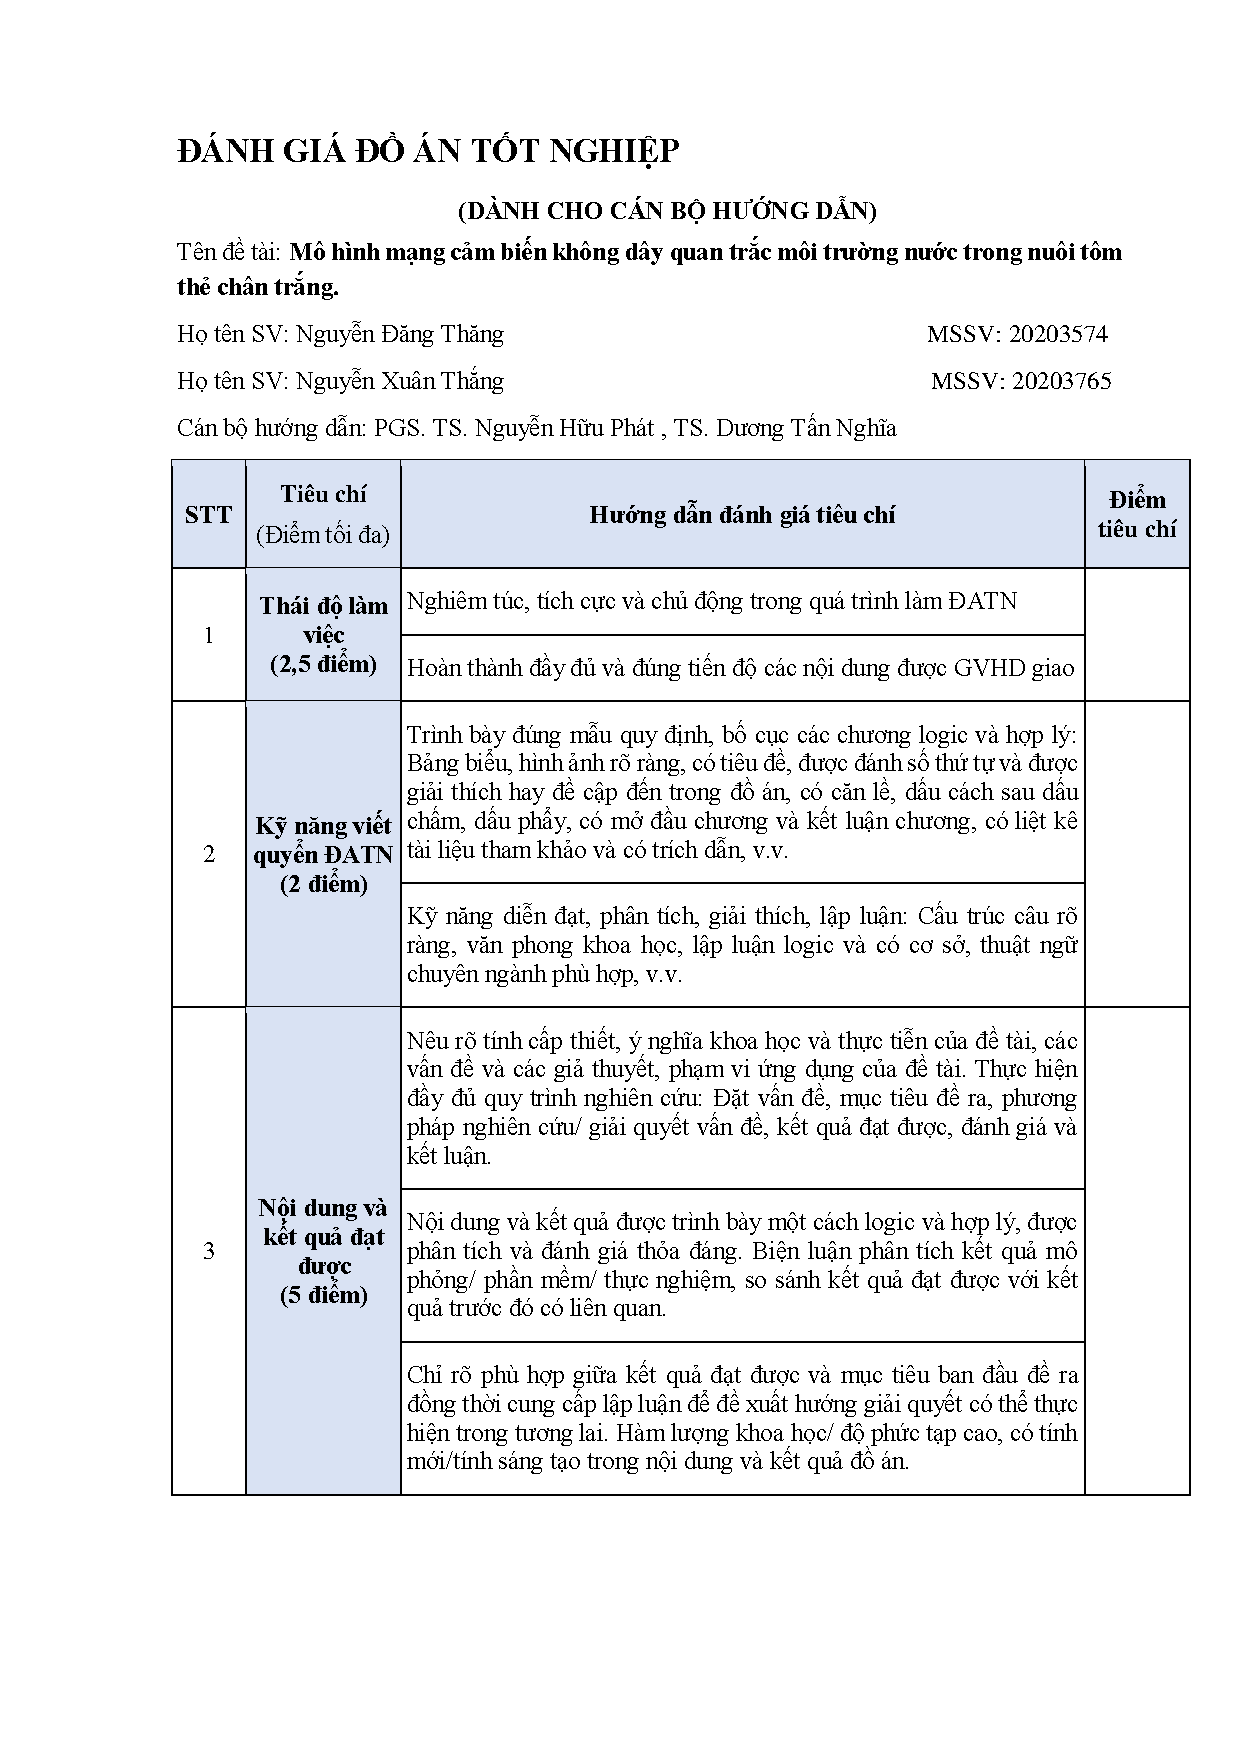
\includepdf[scale=1,pages=-]{EvaluationCriteria/danhgiadoan.pdf}
	\section*{LỜI NÓI ĐẦU}
\thispagestyle{empty}
Trong bối cảnh hội nhập hiện nay, các quốc gia đang cùng nhau tiến vào thời đại công nghệ 4.0, nơi vạn vật đều được kết nối và mọi khía cạnh của xã hội đều được lan tỏa và cải tiến nhờ sự phát triển mạnh mẽ của công nghệ thông tin và trí tuệ nhân tạo. Đặc biệt, trước thách thức của biến đổi khí hậu, việc ứng dụng công nghệ để bảo vệ và quản lý nguồn tài nguyên nước ngày càng trở nên cấp thiết.

Ngành nuôi trồng thủy sản đang phát triển mạnh mẽ tại Việt Nam. Việc đầu tư vào các dự án nuôi trồng thủy hải sản ngày càng lớn, nhưng đồng thời cũng đối mặt với nhiều thách thức và rủi ro, đặc biệt là về môi trường nước. Ngay gần đây đài truyền hình VTV có đăng bản tin vào tháng 4 vừa qua hàng trăm tấn cá chết tại Hải Dương. Cho thấy khả năng tác động của thời tiết và biến đổi khí hậu ảnh hưởng lớn đên thế nào. Các loại thủy sản tôm sú, cá biển mang lại lợi nhuận cao, nhưng lại dễ gây thiệt hại cho người dân nếu không được nuôi trồng đúng cách và xử lý nhanh tác động của môi trường. Trong quá trình nuôi trồng thủy sản, nguồn nước đóng vai trò then chốt, ảnh hưởng trực tiếp đến sự sống và phát triển của các loài thủy sản. Vì vậy, việc giám sát môi trường nước thường xuyên để kịp thời phát hiện và xử lý nhanh chóng các hiện tượng bất lợi khi môi trường thay đổi là vô cùng cần thiết. Hiện nay, kiểm tra chất lượng nước tại các hồ nuôi thủy sản vẫn chủ yếu được thực hiện bằng phương pháp thủ công, sử dụng các thiết bị chất lượng thấp. Tuy nhiên, với kiến thức đã học trên giảng đường và mong muốn đóng góp vào lĩnh vực này, Chúng em quyết định lựa chọn đề tài \textbf{" Mô hình mạng cảm biến không dây quan trắc môi trường nước trong nuôi tôm chân trắng"} làm đề tài tốt nghiệp của mình. Trong quá trình tìm hiểu,  chúng em nhận thấy rằng các yếu tố như nhiệt độ, nồng độ pH, độ mặn, nồng độ oxi của nước rất quan trọng trong quá trình nuôi trồng thủy sản. Nếu các thông số này thay đổi mà người nuôi không nắm bắt được thông tin kịp thời, sẽ phải đối mặt với những hậu quả nghiêm trọng. Vì vậy, em đã quyết định xây dựng hệ thống mạng cảm biến không dây khả năng quan trắc, đo lường các thông số. Đây là một giải pháp hữu ích và tiên tiến giúp cải thiện hiệu quả trong việc quản lý nuôi trồng thủy hải sản và đảm bảo sự bền vững của ngành này trong tương lai.
\cleardoublepage
 % Lời nói đầu.
	
	\section*{LỜI CẢM ƠN}
Em xin gửi lời cảm ơn đến \textbf{ PGS. TS. Nguyễn Hữu Phát, TS. DƯƠNG TẤN NGHĨA} đã hướng dẫn em rất nhiệt tình, đầy đủ về mặt kiến thức, kỹ thuật, phương pháp tiếp cận. Bên cạnh đó, em xin gửi lời cảm ơn tới sự trợ giúp của các thành viên ở phòng nghiên cứu SANSLAB 713 toà nhà C7. Cuối cùng, em xin cảm ơn thầy cô trường Điện-Điện tử đã tận tình giảng dạy và truyền đạt kiến thức cho chúng em. 

Do kiến thức và thời gian nghiên cứu hạn hẹp nên đồ án của em không thể tránh khỏi những thiếu sót khi trình bày và đánh giá về vấn đề trong đồ án. Em mong có thể nhận được những ý kiến, nhận xét của thầy cô để em có thể hoàn thiện và phát triển đồ án tốt nghiệp mang tính ứng dụng cao hơn trong cuộc sống. 

\vspace{10pt}
\hspace{8.7cm}Em xin chân thành cảm ơn !
\thispagestyle{empty}
\clearpage


\section*{LỜI CAM ĐOAN}
\thispagestyle{empty}
Tôi tên là NGUYÊN ĐĂNG THĂNG, mã số sinh viên 20203574, sinh viên lớp ĐTVT 06, khóa K65. Tôi tên là NGUYỄN XUÂN THẮNG, mã số sinh viên 20203765, sinh viên lớp DTVT 01, khóa K65. Người hướng dẫn là \textbf{PGS. TS. NGUYỄN HỮU PHÁT, TS. DƯƠNG TẤN NGHĨA}. Chúng tôi xin cam đoan toàn bộ nội dung được trình bày trong đồ án \textbf{"Mô hình mạng cảm biến không dây quan trắc môi trường nước trong nuôi tôm thẻ chân trắng"} là kết quả quá trình tìm hiểu và nghiên cứu của tôi. Các dữ liệu được nêu trong đồ án là hoàn toàn trung thực, phản ánh đúng kết quả đo đạc thực tế. Mọi thông tin trích dẫn đều tuân thủ các quy định về sở hữu trí tuệ; các tài liệu tham khảo được liệt kê rõ ràng. Tôi xin chịu hoàn toàn trách nhiệm với những nội dung được viết trong đồ án này.

\vspace{6pt}
\hspace{7cm}Hà Nội, ngày 8 tháng 7 năm 2024

\hspace{9cm}\textbf{Người cam đoan}

\vspace{1.5cm}
\hspace{8cm}\textbf{NGUYỄN ĐĂNG THĂNG}\\
\vspace{1cm}
\hspace{8.87cm}\textbf{NGUYỄN XUÂN THẮNG}

\clearpage

\newpage
\begin{table}[H]
\begin{tabular}{|l|l|cc|}
	\hline
	\multirow{2}{*}{Công việc}                                                                    & \multirow{2}{*}{Mô tả chi tiết}                                                                                                             & \multicolumn{2}{l|}{Người thực hiện}                    \\ \cline{3-4} 
	&                                                                                                                                             & \multicolumn{1}{l|}{Thắng} & \multicolumn{1}{l|}{Thăng} \\ \hline
	\multirow{3}{*}{\begin{tabular}[c]{@{}l@{}}Tìm kiếm nghiên\\  cứu liên quan\end{tabular}}     & \begin{tabular}[c]{@{}l@{}}Tìm hiểu thực trạng nuôi \\ tôm chân trắng ở Việt Nam\end{tabular}                                               & \multicolumn{1}{c|}{X}     & X                          \\ \cline{2-4} 
	& \begin{tabular}[c]{@{}l@{}}Tìm hiểu các nghiên cứu về \\ thiết bị quan trắc môi trường nuôi tôm\end{tabular}                                & \multicolumn{1}{c|}{X}     &                            \\ \cline{2-4} 
	& \begin{tabular}[c]{@{}l@{}}Tìm hiểu các nghiên cứu \\ về truyền thông trong mạng Iot\end{tabular}                                           & \multicolumn{1}{c|}{}      & X                          \\ \hline
	\multirow{2}{*}{\begin{tabular}[c]{@{}l@{}}Lập danh sách, \\ khảo sát linh kiện\end{tabular}} & \begin{tabular}[c]{@{}l@{}}Lên danh sách linh kiện \\ cho thiết bị đo (node)\end{tabular}                                                   & \multicolumn{1}{c|}{X}     &                            \\ \cline{2-4} 
	& \begin{tabular}[c]{@{}l@{}}Lên danh sách linh kiện \\ cho thiết bị trung tâm (gateway)\end{tabular}                                         & \multicolumn{1}{c|}{}      & X                          \\ \hline
	\multirow{2}{*}{Xây dựng hệ thống}                                                            & \begin{tabular}[c]{@{}l@{}}Thiết kế lưu đồ thuật toán \\ của thiết bị node\end{tabular}                                                     & \multicolumn{1}{c|}{X}     &                            \\ \cline{2-4} 
	& \begin{tabular}[c]{@{}l@{}}Thiết kế lưu đồ thuật toán \\ của gateway\end{tabular}                                                           & \multicolumn{1}{c|}{}      & X                          \\ \hline
	\multirow{2}{*}{Thiết kế mạch cứng}                                                           & \begin{tabular}[c]{@{}l@{}}Thiết kế các khối cho quá \\ trình quan trắc đo đạc\end{tabular}                                                 & \multicolumn{1}{c|}{X}     &                            \\ \cline{2-4} 
	& Thiết kế các khối truyền thông                                                                                                              & \multicolumn{1}{c|}{}      & X                          \\ \hline
	\multirow{2}{*}{Thiết kế vỏ hộp}                                                              & Thiết kế vỏ hộp cho thiết bị Node                                                                                                           & \multicolumn{1}{c|}{X}     &                            \\ \cline{2-4} 
	& Thiết kế vỏ hộp cho Gateway                                                                                                                 & \multicolumn{1}{c|}{}      & X                          \\ \hline
	Hoàn thiện sản phẩm                                                                           & \begin{tabular}[c]{@{}l@{}}Hàn, gắn và thử nghiệm các khối\\ như đã thiết kế, lắp lắp vào vỏ hộp\end{tabular}                               & \multicolumn{1}{c|}{X}     & X                          \\ \hline
	\begin{tabular}[c]{@{}l@{}}Thực hiện hiệu chỉnh \\ thiết bị đo\end{tabular}                   & \begin{tabular}[c]{@{}l@{}}Thực hiện lấy dung dịch chuẩn, hiệu \\ chỉnh thông số cảm biến \\ pH, DO, EC, nhiệt độ\end{tabular}              & \multicolumn{1}{c|}{X}     &                            \\ \hline
	\begin{tabular}[c]{@{}l@{}}Thực hiện lấy thông\\ số truyền thông\end{tabular}                 & \begin{tabular}[c]{@{}l@{}}Thực hiện lấy dữ liệu SNR, lost, RSSI, \\ theo khoảng cách đối với từng hệ \\ số trải phổ khác nhau\end{tabular} & \multicolumn{1}{c|}{}      & X                          \\ \hline
	Thực nghiệm                                                                                   & \begin{tabular}[c]{@{}l@{}}Triển khải bộ đo thực tế và khảo \\ sát vị trí cho thiết bị truyền thông\end{tabular}                            & \multicolumn{1}{c|}{X}     & X                          \\ \hline
	Đánh giá                                                                                      & Đánh giá toàn bộ kết quả đạt được                                                                                                           & \multicolumn{1}{c|}{X}     & X                          \\ \hline
\end{tabular}
\end{table}
\thispagestyle{empty}
\clearpage % Lời cam đoan.
	% Tạo mục lục tự động
	\addtocontents{toc}{\protect\thispagestyle{empty}}
	\tableofcontents
	\thispagestyle{empty}
	\cleardoublepage
	
	
	
	
	\pagenumbering{roman} % Đánh số thứ tự la mã
\section*{DANH MỤC KÝ HIỆU VÀ CHỮ VIẾT TẮT}
\phantomsection \addcontentsline{toc}{section}{\numberline {} DANH MỤC KÝ HIỆU VÀ CHỮ VIẾT TẮT}


	\begin{tabular}{lll}
		IoT        & Internet of Things                                                                              & Internet kết nối vạn vật                                                                \\
		RTOS       & Real-Time Operating System                                                                      & Hệ điều hành thời gian thực                                                             \\
		GIS        & Geographic Information System                                                                   & Hệ thống thông tin địa lý                                                               \\
		DO         & Dissolved Oxygen                                                                                & Độ oxy hòa tan                                                                          \\
		QCVN       &                                                                                                 & Quy chuẩn Việt Nam                                                                      \\
		TT-BNNPTNT &                                                                                                 & \begin{tabular}[c]{@{}l@{}}Thông tư Bộ nông nghiệp \\ phát triển nông thôn\end{tabular} \\
		NTC        & Negative Temperature Coefficient                                                                & Hệ số nhiệt độ âm                                                                       \\
		ISE        & Ion selective electrode                                                                         & Điện cực chọn lọc Ion                                                                   \\
		ADC        & Analog Digital Converter                                                                        & \begin{tabular}[c]{@{}l@{}}Bộ chuyển đổi tín hiệu\\  tương tự sang số\end{tabular}      \\
		BW         & Bandwidth                                                                                       & Băng thông                                                                              \\
		LPWAN      & Low Power Wide Area Network                                                                     & Mạng diện rộng năng lượng thấp                                                          \\
		CR         & Coding Rate                                                                                     & Tỷ lệ mã hóa                                                                            \\
		CSS        & Chirp Spread Spectrum                                                                           & Kỹ thuật trải phổ chirp                                                                 \\
		FSK        & Frequency Shift Key                                                                             & Kỹ thuật Chuyển Tần số                                                                  \\
		LoRa       & Long range                                                                                      & Phạm vi xa                                                                              \\
		MAC        & Medium Access Control                                                                           & Điều khiển truy cập                                                                     \\
		MCU        & Microcontroller Unit                                                                            & Vi điều khiển                                                                           \\
		RAM        & Random Access Memory                                                                            & Bộ nhớ truy cập ngẫu nhiên                                                              \\
		WSN        & Wireless Sensor Network                                                                         & Mạng cảm biến không dây                                                                 \\
		MQTT       & MQ Telemetry Transport                                                                          &                                                                                         \\
		HTTP       & Hypertext Transfer Protocol                                                                     & Giao thức Truyền tải Siêu văn bản                                                       \\
		CoAP       & Constrained Application Protocol                                                                &                                                                                         \\
		SF         & Spreading Factor                                                                                & Hệ số lan truyền                                                                        \\
		I2C        & Inter-Integrated Circuit                                                                        &                                                                                         \\
		SPI        & Serial Peripheral Interface                                                                     &                                                                                         \\
		UART       & \begin{tabular}[c]{@{}l@{}}Universal asynchronous \\ receiver/transmitte\end{tabular} &                                                                                        
	\end{tabular}


\newpage
 % Danh mục ký hiệu và chữ viết tắt
	
	%Tạo danh mục hình vẽ.
	{\let\oldnumberline\numberline
		\renewcommand{\numberline}{Hình~\oldnumberline}
		\listoffigures} 
	\phantomsection\addcontentsline{toc}{section}{\numberline {} DANH MỤC HÌNH VẼ}
	\newpage
	
	%Tạo danh mục bảng biểu.
	{\let\oldnumberline\numberline
		\renewcommand{\numberline}{Bảng~\oldnumberline}
		\listoftables}
	\phantomsection\addcontentsline{toc}{section}{\numberline {} DANH MỤC BẢNG BIỂU}
	\newpage
	
	\section*{TÓM TẮT ĐỒ ÁN}
\phantomsection\addcontentsline{toc}{section}{\numberline {}TÓM TẮT ĐỒ ÁN}
Đồ án tốt nghiệp được thực hiện xuất phát từ quá trình học tập và nghiên cứu xu hướng công nghệ hiện đại, ứng dụng vào thực tế với những thiết kế tối ưu nhất và lòng yêu quê hương nơi mình sinh ra. Nội dung của đồ án giải quyết bài toán thiết kế một hệ thống mạng cảm biến không dây nhận dữ liệu đo đạc các thông số môi trường nuôi tôm từ nhiều ao nuôi, mở rộng ra là có thể hoạt động riêng lẻ từng bộ đo đối với hộ gia đình quy mô nhỏ, hoạt động ổn định và liên tục trong việc thực hiện giám sát các thông số từ xa với nhiều thiết bị tại mọi vị trí trên bản đồ. Để có thể giải quyết tốt bài toán trên em đã tham khảo nhiều nguồn mở, kinh nhiệm của các anh chị đi trước và một số bài báo để tìm ra thông số môi trường nước nuôi tôm cần thiết và phần cứng phù hợp với vấn đề đặt ra. Trong quá trình đó vấn đề liên quan đến cảm biến, cụ thể là lấy mẫu các dung dịch chuẩn tìm được giải giải quyết vấn đề nhiễu trong môi trường nước giữa các cảm biến, khả năng hoạt động ổn định là theo dõi liên tục tại các địa phương nơi hệ thống điện không ổn định, diện tích ao nuôi cách xa nhau, vấn đề nền tảng IoT lưu trữ dữ liệu sử dụng nền tảng có sẵn hỗ trợ API để đấy dữ liệu và hiển thị dữ liệu. 

Đồ án có ý tưởng về một hệ thống mạng cảm biến không dây theo dõi các thông số môi trường nước như nhiệt độ, pH, độ mặn, DO, lấy dữ liệu vị trí đo, thời gian được hiển thị tại bất kì địa điểm nào trên bản đồ, hệ thống được cung cấp nguồn adapter và pin Lithium có thể sạc được nhờ năng lượng mặt trời và có thể đặt tại bất kì địa điểm nào. Có thể ứng dụng vào các hộ gia đình lớn hoặc quy mô nhỏ, địa phương có lưới điện không ổn định, nhưng cần có một số cải tiến trong tương lai như: đưa ra các thông số dự đoán sớm nhờ mô hình AI tiên tiến, tích hợp một phần cứng nhằm giải quyết nhanh chóng vấn đề thông số nước khi khí hậu thất thường như hiện nay.
\clearpage

\section*{ABSTRACT}

The graduation project was initiated from the process of studying and researching modern technological trends, applying them in practice with the most optimal designs and a love for the homeland where I was born. The content of the project addresses the problem of designing a wireless sensor network system to receive measurement data of environmental parameters in shrimp farming ponds, which can be expanded to operate individually for small-scale households, operating stably and continuously in monitoring parameters remotely with multiple devices at any location on the map. To effectively solve this problem, I have referred to many open sources, the experience of predecessors, and several articles to identify the necessary water environment parameters for shrimp farming and the appropriate hardware for the given issue. During this process, issues related to sensors, specifically sampling standard solutions to solve the problem of noise in the water environment among sensors, ensuring stable operation through continuous monitoring in localities with unstable power systems and ponds spread over large areas, and using IoT platforms to store data with available platforms supporting APIs for data pushing and display were addressed.

The project envisions a wireless sensor network system that monitors water environment parameters such as temperature, pH, salinity, and DO, capturing the measurement location and time displayed at any location on the map. The system is powered by an adapter and rechargeable Lithium battery via solar energy and can be placed at any location. It can be applied to both large and small-scale households and localities with unstable power grids but requires some future improvements such as early prediction parameters using advanced AI models and integrating hardware to quickly address water parameter issues due to current erratic climate changes.

\cleardoublepage

\newpage
\section*{PHẦN MỞ ĐẦU}

Trong đồ án này, em tập trung xây dựng hệ thống gồm hai node và một gateway. Node cảm biến thu thập dữ liệu các thông số môi trường: độ mặn, pH, DO, nhiệt độ. Gateway thu thập dữ liệu gửi từ node thông qua Lora, được lưu trữ trên máy chủ (Server), dữ liệu từ hệ thống được quan sát thông qua bản đồ GIS, hoặc trực tiếp trên màn hình thiết bị đo. Được cung cấp điện áp ổn định và lâu dài trong quá trình theo dõi dữ liệu, di chuyển và lắp đặt dễ dàng. Trong quá trình tìm hiểu, em đã kết hợp tài liệu từ nhiều nguồn như báo nghiên cứu khoa học, các đồ án của các anh chị đi trước và tham khảo các trang web để có kiến thức hoàn thiện đề tài.

Nội dung trình bày đồ án tốt nghiệp gồm 3 chương:
\begin{itemize}[label= $\triangleright$]
\item CHƯƠNG 1: Tổng quan về hệ thống mạng cảm biến không dây đo thông số nước
    Trình bày tổng quát về đề tài, tính cấp thiết, đặt vấn đề, mục đích nghiên cứu, các công trình nghiên cứu liên quan, phương pháp và đề xuất hệ thống.
\item CHƯƠNG 2: Cơ sở lý thuyết
    Giới thiệu tổng quan về IoT, các thành phần của IoT, giao thức truyền thông IoT, ảnh hưởng các thông số nước đến với môi trường nuôi tôm.
\item CHƯƠNG 3: Xây dựng hệ thống, thử nghiệm và đánh đánh giá kết quả đạt được
    Trình bày chi tiết phương pháp thực hiện, phân tích, thiết kế sơ đồ khối hệ thống và sơ đồ của từng khối, khối thành phần để xây dựng hệ thống đo thông số môi trường nước. Trình bày phương pháp đánh giá độ chính xác, sai số và hạn chế của các phần cứng nhằm đánh giá kết quả đạt được.
\end{itemize}

\cleardoublepage % Tóm tắt đồ án 
	\cleardoublepage
	
	
	\pagenumbering{arabic} % Đánh số thứ tự 1,2,3...
	\section*{CHƯƠNG 1. TỔNG QUAN}
	\addcontentsline{toc}{section}{\numberline{}CHƯƠNG 1. TỔNG QUAN}
	\setcounter{section}{1}
	\setcounter{figure}{0}
	\setcounter{table}{0}
	Trong chương này, em trình bày tổng quan về tính cấp thiết của đề tài, đặt vấn đề, mục đích nghiên cứu, phạm vi đề tài, nhiệm vụ nghiên cứu. Ngoài ra, em sẽ trình bày các hướng nghiên cứu, các công trình nghiên cứu liên quan đã được công bố mà em tham khảo. Từ đó đề xuất các chức năng và yêu cầu của hệ thống.
	
	\subsection{Tính cấp thiết của đề tài}
	Việt Nam là một quốc gia phát triển nhanh chóng, với ngành xuất khẩu tôm đóng vai trò vô cùng quan trọng trong bối cảnh xuất nhập khẩu thủy sản toàn cầu. Theo thống kê của Cục thủy sản \cite{Thuysan}, trong 6 tháng đầu năm 2023, tôm Việt Nam đã xuất khẩu sang 84 thị trường trên thế giới, với kim ngạch đạt hơn 1,5 tỷ USD, riêng trong tháng 6/2023, xuất khẩu tôm đạt 328,9 triệu USD. Theo khảo sát từ tỉnh Sóc Trăng \cite{SocTrang}, người nuôi tôm phải nuôi theo thời vụ để đảm bảo năng suất cao, vì thế chất lượng nuôi tôm phụ thuộc lớn vào thời tiết. 
	
	\begin{figure}[!ht]
		\centering
		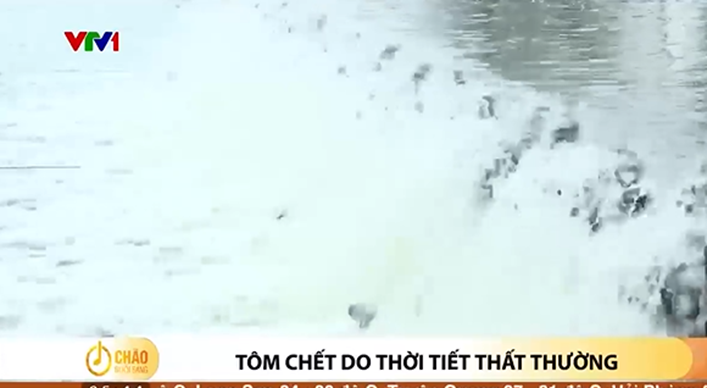
\includegraphics[width=11cm,height=6cm]{Images/Problem.png}
		\caption[Bản tin chào buối sáng 10/6/2024 tại VTV1\cite{VTVGo} ]{\bfseries \fontsize{12pt}{0pt}\selectfont Bản tin chào buối sáng 10/6/2024 tại VTV1\cite{VTVGo}}
		\label{Problem}
	\end{figure}
	
	Bản tin Hình \ref{Problem} vào tháng 10/6 đài truyền hình VTV có đăng 1 phóng sự \cite{VTVGo} về nắng nóng kéo dài với nền nhiệt độ cao, xen kẽ các đợt mưa lớn đột ngột, hiện tượng thời tiết bất thường này khiến người nuôi tôm hết sức lo lắng, tại nhiều vùng nuôi tôm ở Nghệ An đã xảy ra dịch bệnh, làm cho tôm chết hàng loạt.
	
	Các nghiên cứu khác cũng chỉ ra rằng chất lượng môi trường nuôi tôm ảnh hưởng lớn đến sức khỏe của tôm, đặc biệt là loại tôm chân trắng. Do đó, người nuôi tôm cần theo dõi sát sao môi trường nuôi để đảm bảo năng suất cao và phòng ngừa các tác hại xấu.
	Trong bối cảnh hội nhập và sự bùng nổ của cuộc cách mạng công nghiệp 4.0, các mô hình IoT đang phát triển mạnh mẽ, mang đến những giải pháp thông minh thế hệ mới cho mọi lĩnh vực của đời sống. Đối với ngành nuôi trồng thủy sản, việc sử dụng hệ thống theo dõi môi trường nuôi tôm được coi là sẽ mang lại giá trị hiệu quả và bền vững lâu dài. Nhờ theo dõi và nắm bắt chính xác thông tin về thông số môi trường nước trong ao nuôi, người chăn nuôi có thể tối ưu hóa quy trình nuôi tôm, giảm thiểu thời gian, tăng năng suất và hạn chế các tác động xấu từ môi trường tự nhiên.
	Tuy nhiên, qua khảo sát thị trường về các thiết bị đo chất lượng nước, thực trạng cho thấy giá thành của các thiết bị này rất cao và tính áp dụng chưa cao.
	
	Từ thiết bị ở Hình \ref{maydo}, ta có thể thấy thiết bị HACH HQ40d xuất xứ Hoa Kỳ là thiết bị đo cầm tay. Theo trang giới thiệu \cite{HannaHI9829}, đây là thiết bị có thể đo được nhiều thông số của môi trường nước. Tuy nhiên việc giám sát liên tục các thông số ở hồ nuôi tôm với thiết bị này sẽ mất rất nhiều thời gian và công sức. Người chăn nuôi sẽ phải lấy trực tiếp mẫu nước hàng ngày để tự tay đo. Ngoài ra thiết bị có giá thành cao cho người nông dân để có thể sử dụng được. 
	
	\begin{figure}[!ht]
		\centering
		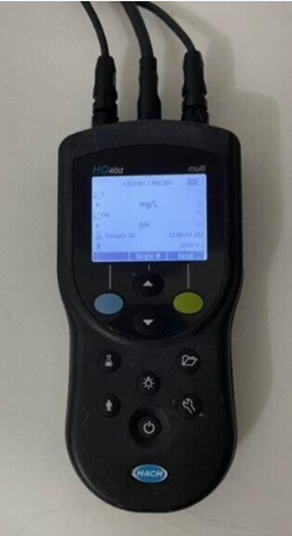
\includegraphics[width=4cm,height=6cm]{Images/maydo.png}
		\caption[Máy đo chất lượng nước đa chỉ tiêu Hanna HI9829 giá 42.482.000 đồng \cite{HannaHI9829} ]{\bfseries \fontsize{12pt}{0pt}\selectfont Máy đo chất lượng nước đa chỉ tiêu Hanna HI9829 giá 42.482.000 đồng \cite{HannaHI9829}}
		\label{maydo}
	\end{figure}
	
	Đối với thiết bị ở Hình \ref{giamsat}, đây là một thiết bị đo thông số nước tự động của hãng EPLUSI - một sản phẩm đến từ Việt Nam, thông số nước có thể được đo tự động và được quản lý từ xa. Tuy nhiên với nhu cầu lớn về nhiều thiết bị được lắp trên nhiều 1 ao nuôi hoặc xa hơn là nhiều ao nuôi thì giá thành sẽ bị đẩy rất cao để triển khai cho nhà nông.
	
	\begin{figure}[!ht]
		\centering
		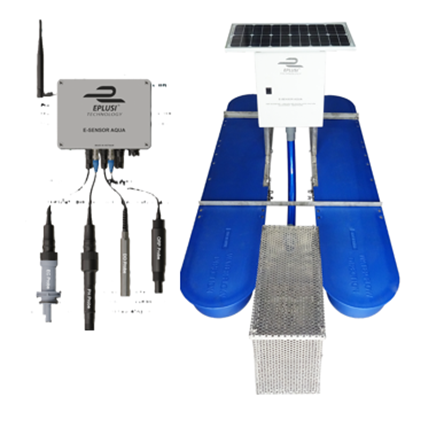
\includegraphics[width=7cm,height=5.5cm]{Images/giamsat.png}
		\caption[Hệ thống giám sát môi trường nước \cite{E-SENSORAQUA} ]{\bfseries \fontsize{12pt}{0pt}\selectfont Hệ thống giám sát môi trường nước \cite{E-SENSORAQUA}}
		\label{giamsat}
	\end{figure}
	
	Ngoài ra, em đã khảo sát tuy trong và ngoài nước đã có rất nhiều máy đo chất lượng nước nhưng đặc điểm chung là giá thành của 1 thiết bị đo là rất cao và hầu như cũng chưa có một hệ thống giúp cho người dân có thể theo dõi được nhiều thiết bị trên nhiều ao của vùng nuôi. 
	
	Hệ thống mạng cảm biến giám không dây giám sát môi trường nuôi tôm thông minh chắc chẵn vẫn sẽ luôn là một đề tài nhận được sự quan tâm không chỉ trong nước và quốc tế bởi tính cấp thiết và những lợi ích mà hệ thống mang lại. Do đó với những kiến thức đã được học trên trường cũng như các kiến thức được trải nghiệm thực tế, em đã chọn đề tài \textbf{ “Mô hình mạng cảm biến không dây quan trắc môi trường nước trong nuôi tôm chân trắng” }làm đề tài tốt nghiệp của mình.
	
	\subsection{Mục đích nghiên cứu}
	Xây dựng một hệ thống mạng cảm biến không dây theo dõi và thu thập các thông số nước tự động,trực quan hóa dữ liệu tại nền tảng website IoT.
	\subsection{Phạm vi đề tài}
	Đề tài ứng dụng chính vào việc thu thập dữ liệu quan trắc thông số môi trường nước tại các ao nuôi của người dân. Kết nối dữ liệu đo đạc từ nhiều ao tới thiết bị tổng, theo dõi và nắm bắt tình hình các hồ nuôi một cách thuận tiện nhất.
	
	\subsection{Nội dung nghiên cứu}
	\begin{itemize}
		\item Khảo sát linh kiện và tối ưu phần cứng.
		\item Thiết kế mạch phần cứng.
		\item Mô hình mạng đa node cho hệ thống IOT.
		\item Triển khai thử nghiệm.
	\end{itemize}
	
	\subsection{Các nghiên cứu liên quan}
	
	\subsubsection{Thiết bị đo}
	
	\paragraph{Nguồn điện năng lượng mặt trời}\mbox{}
	
	Năng lượng mặt trời là dạng năng lượng bền vững, tái tạo và rất sạch. Do thiếu hụt nghiêm trọng các dạng năng lượng không tái tạo, cần phải khai thác năng lượng mặt trời. Trong hai thập kỷ qua, việc thu thập năng lượng mặt trời đã trở thành một chủ đề nóng. Nhiều tổ chức nghiên cứu trên thế giới đang tập trung vào cách khai thác năng lượng mặt trời một cách tối ưu. Một tế bào năng lượng mặt trời hoạt động bằng cách chuyển đổi ánh sáng thành điện. Năng lượng điện này có thể được sử dụng để chạy các tải khác nhau và sạc pin \cite{qin2012matlab}.
	
	Tế bào năng lượng mặt trời có đặc tính đầu ra phi tuyến tính được gọi là đặc tính điện áp (IV) và mảng quang điện (PV). Những đặc tính này là hàm của ánh sáng, nhiệt độ và điện áp đầu ra của mô-đun PV. Do đó, đường cong là phi tuyến tính. Do đó, cần phải làm cho tế bào hoạt động tại điểm công suất tối đa để có thể được sử dụng cho các ứng dụng hệ thống PV khác nhau. Ngoài ra, tính chất của các đường cong này xác định hiệu suất của tấm pin. Có ba yếu tố quan trọng xác định hiệu suất - hiệu suất của tấm pin, hiệu suất của mạch chuyển đổi và hiệu suất của thuật toán theo dõi điểm công suất tối đa (MPPT). Không dễ để cải thiện hiệu suất của tấm pin và mạch chuyển đổi. Cách tốt nhất để cải thiện hiệu suất tổng thể là thiết kế một thuật toán hiệu quả để theo dõi công suất tối đa. Ngoài ra, năng lượng được tạo ra thông qua hiệu ứng quang điện không thể được sử dụng trực tiếp để cung cấp năng lượng cho hầu hết các mạch điện tử trong Hình \ref{tampin}.
	
	\begin{figure}[!ht]
		\centering
		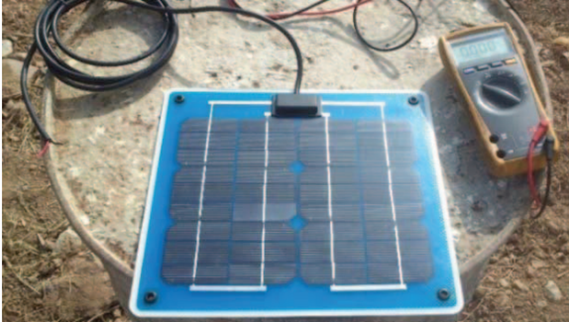
\includegraphics[width=7cm,height=4cm]{Images/tampin.png}
		\caption[Tấm pin mặt trời GPDL5\cite{batt2022design}]{\bfseries \fontsize{12pt}{0pt}\selectfont Tấm pin mặt trời GPDL5\cite{batt2022design} }
		\label{tampin}
	\end{figure}
	
	\paragraph{Nghiên cứu về tế bào năng lượng mặt trời}\mbox{}
	
	Khi ánh sáng mặt trời chiếu vào bề mặt tế bào năng lượng mặt trời, các lỗ trống và electron được tạo ra. Các lỗ trống và electron được tách ra bởi trường nội tại được tạo ra tại mối nối \cite{batt2022design}. Các lỗ trống di chuyển vào lớp p và các electron vào lớp n. Khi mạch được đóng, các electron tự do đi qua tải và do đó tạo ra dòng điện. Do đó, điện được tạo ra từ các tế bào năng lượng mặt trời dưới ánh sáng như được minh họa trong Hình \ref{nltampin}
	
	\begin{figure}[!ht]
		\centering
		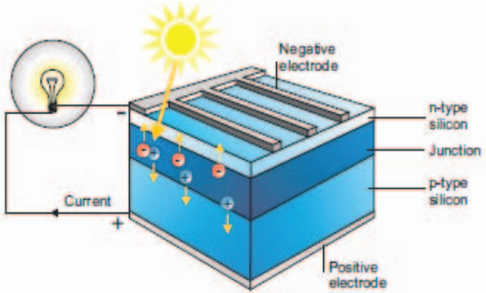
\includegraphics[width=7cm,height=4cm]{Images/nltampin.png}
		\caption[ Nguyên lý hoạt động của pin mặt trời \cite{batt2022design}]{\bfseries \fontsize{12pt}{0pt}\selectfont Nguyên lý hoạt động của pin \cite{batt2022design}}
		\label{nltampin}
	\end{figure}
	
	\newpage
	Nếu bây giờ tải RL được kết nối như được trình bày trong Hình \ref{quangdien}, một phần dòng điện cũng sẽ chạy qua tải và điện áp trên thiết bị giảm. Trong bóng tối, nó hoạt động như một điốt đơn giản và do đó không tạo ra dòng điện nào \cite{batt2022design}.
	
	\begin{figure}[!ht]
		\centering
		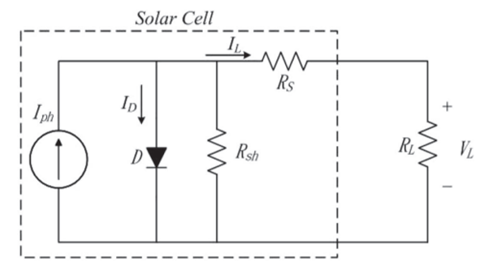
\includegraphics[width=7cm,height=4cm]{Images/quangdien.png}
		\caption[ Mạch tương đương của pin quang điện \cite{batt2022design}]{\bfseries \fontsize{12pt}{0pt}\selectfont Mạch tương đương của pin quang điện \cite{batt2022design} }
		\label{quangdien}
	\end{figure}
	
	Năng lượng mặt trời có sẵn miễn phí nhưng chi phí để khai thác năng lượng này rất cao. Vì vậy, cần phải vận hành ở điểm công suất tối đa (MPP). Tế bào PV tốt nhất có hiệu suất lên đến 30\%. Do đó, công suất đầu ra nhỏ so với lượng đầu vào cần thiết. Vì tế bào PV có đặc tính I-V và P-V phi tuyến tính, cần thiết kế một mạch điều khiển hoặc thuật toán để điều chỉnh tế bào hoạt động ở MPP bất kể tải được kết nối. Để cải thiện hiệu suất của tấm pin mặt trời, sử dụng Hệ thống Theo dõi Điểm Công suất Tối đa (MPPT). Theo định lý điểm công suất tối đa, khi trở kháng tải bằng trở kháng nguồn hoặc tổng trở của mạng khi nhìn từ tải, công suất đầu ra đạt được là lớn nhất. Vì vậy, nói chung vai trò của thuật toán MPPT là giải quyết vấn đề khớp trở kháng như Hình \ref{htPv} \cite{batt2022design}. 
	
	\begin{figure}[!ht]
		\centering
		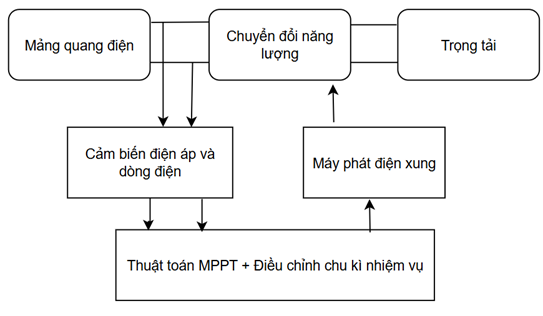
\includegraphics[width=7cm,height=4cm]{Images/htPv.png}
		\caption[ Sơ đồ khối của hệ thống PV \cite{batt2022design}]{\bfseries \fontsize{12pt}{0pt}\selectfont  Sơ đồ khối của hệ thống PV \cite{batt2022design} }
		\label{htPv}
	\end{figure}
	
	Trong sơ đồ trên, bộ chuyển đổi Buck-Boost \cite{batt2022design},  được sử dụng như một thiết bị khớp trở kháng giữa đầu vào và đầu ra bằng cách thay đổi chu kỳ làm việc của mạch chuyển đổi. Mạch MPPT lấy điện áp và dòng điện sinh ra từ tế bào năng lượng mặt trời và thuật toán tính toán điện áp tham chiếu, từ đó điều chỉnh chu kỳ làm việc.
	
	\paragraph{Ứng dụng năng lượng mặt trời vào hệ thống IoT}\mbox{}
	
	Các nguồn năng lượng đang đối mặt với sự chuyển đổi nhanh chóng trên toàn thế giới. Xu hướng thay đổi này giữa nhiên liệu hóa thạch và năng lượng tái tạo chủ yếu được điều khiển bởi nhu cầu năng lượng ngày càng tăng, những lo ngại về môi trường và yêu cầu công nghệ xanh. Trong khi nhiên liệu hóa thạch có thể tiếp tục cung cấp gần 80\% nhu cầu năng lượng tổng cộng cho đến năm 2040, thì năng lượng tái tạo được dự đoán sẽ chiếm hơn 50\% nhu cầu sau đó, với tốc độ tăng trưởng hàng năm hiện tại là 2,5\% \cite{rokonuzzaman2020iot}. Quan niệm này cho thấy một sự quan tâm rõ ràng và tiềm năng của năng lượng tái tạo đối với nhu cầu năng lượng trong tương lai. Trong số các nguồn năng lượng tái tạo tiềm năng, bao gồm năng lượng mặt trời, năng lượng gió, năng lượng sinh khối, năng lượng thủy điện, năng lượng địa nhiệt, năng lượng biển, v.v., năng lượng mặt trời đã nổi lên như một trong ba hình thức năng lượng tái tạo mạnh mẽ nhất.
	
	Mặc dù việc sử dụng năng lượng mặt trời đang mở rộng nhanh chóng, các đặc tính phi tuyến của pin mặt trời đặt ra một thách thức lớn trong việc khai thác công suất tối đa từ năng lượng mặt trời.Tính chất phi tuyến này làm giảm khả năng chuyển đổi năng lượng và tăng chi phí lắp đặt hệ thống. Để khắc phục trở ngại này, các tấm pin phải được vận hành tại điểm công suất cực đại (MPP) dưới các điều kiện khí quyển thay đổi. MPPT  là kĩ thuật theo dõi điểm công suất tối đa là bộ chuyển đổi điện tử để tối ưu hóa sự phù hợp giữa các tấm pin năng lượng mặt trời. Nói một cách đơn giản, chúng chuyển đổi dòng điện DC có điện áp cao hơn từ các tấm pin mặt trời xuống mức điện áp thấp hơn cần thiết để sạc pin hay ắc quy. 
	
	\begin{figure}[!ht]
		\centering
		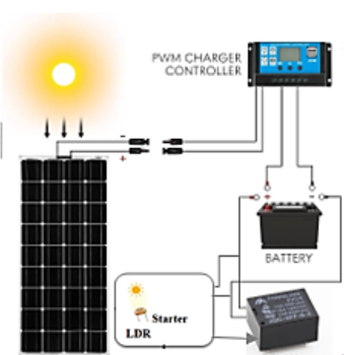
\includegraphics[width=7.3cm,height=4.3cm]{Images/ghepnoimt.png}
		\caption[ Mô hình ghép nối khối nguồn dùng năng lượng mặt trời \cite{el2023developed}]{\bfseries \fontsize{12pt}{0pt}\selectfont Mô hình ghép nối khối nguồn dùng năng lượng mặt trời \cite{el2023developed}}
		\label{ghepnoimt}
	\end{figure}
	
	Mô hình từ nghiên cứu Hình \ref{ghepnoimt} \cite{el2023developed} sử dụng tấm pin mặt trời và ắc quy thông qua bộ điều khiển sạc (PWM charger controller), việc lấy nguồn từ ắc quy hay sử dụng nguồn từ pin thông qua cảm biến quang điện trở (stater LDR) và rơle ghép nối. Việc ứng dụng năng lượng pin mặt trời vào một hệ thống IoT, giúp cho vấn đề lắp đặt tại những nơi thiếu hệ thống lưới điện quốc gia, những nơi cung cấp điện lưới còn bị hạn chế bị cắt thường xuyên mà ánh nắng lại chiếu quanh năm là một giải pháp đột phá.
	
	Trong những đề tài mà việc di chuyển qua lại và lắp đặt tại những vị trí khó tiếp cận điện lưới việc tích hợp pin mặt trời là 1 giải pháp đột phá.
	
	\begin{figure}[!ht]
		\centering
		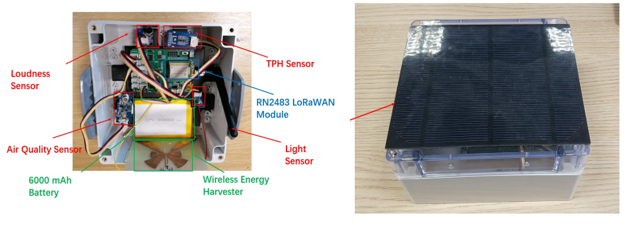
\includegraphics[width=7.7cm,height=4cm]{Images/htthoitiet.png}
		\caption[ Bộ đo theo dõi thông số thời tiết tại thành phố\cite{wang2019new}]{\bfseries \fontsize{12pt}{0pt}\selectfont Bộ đo theo dõi thông số thời tiết tại thành phố\cite{wang2019new}}
		\label{htthoitiet}
	\end{figure}
	
	Hệ thống bao gồm trên của nhóm tác giả Yansong Wang, Yi Huang, and Chaoyun Song \cite{wang2019new} trong Hình \ref{htthoitiet} xây dựng các nút cảm biến không dây, mạng truyền thông và đám mây lưu trữ và hiển thị dữ liệu. Nút cảm biến không dây được cung cấp năng lượng bởi tấm pin năng lượng mặt trời và bộ thu năng lượng tần số vô tuyến (RF) (trong trường hợp năng lượng mặt trời không có sẵn) để tránh thay pin thường xuyên và tiết kiệm chi phí bảo trì. Hệ thống cảm biến thông minh này tích hợp với pin năng lượng mặt trời có thể được sử dụng cho nhiều ứng dụng IoT khác.
	
	\paragraph{Mức độ tin cậy của hệ thống giám sát ao nuôi tôm sử dụng cảm biến đo thông số nước hãng DFRobot}\mbox{}
	
	Đề tài cuả nhóm tác giả Ahmad Zaini, Diah Puspito Wulandari, Retno Wulandari [4]  thiết kế hệ thống giám sát như Hình \ref{sodomach} ao nuôi tôm sử dụng cảm biến pH, DO của hãng DFRobot. 
	
	\begin{figure}[!ht]
		\centering
		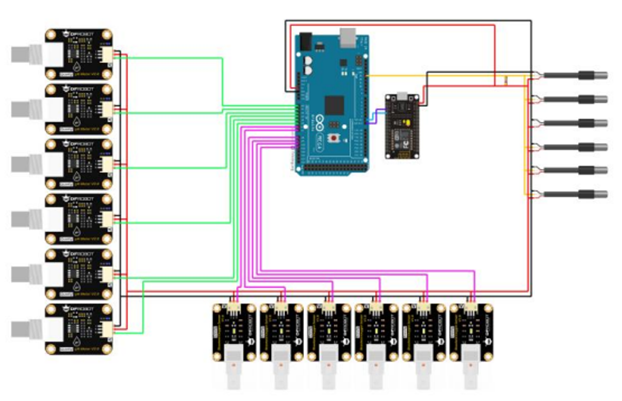
\includegraphics[width=7.4cm,height=4cm]{Images/sodomach.png}
		\caption[ Sơ đồ mạch \cite{zaini2020data}]{\bfseries \fontsize{12pt}{0pt}\selectfont Sơ đồ mạch \cite{zaini2020data}}
		\label{sodomach}
	\end{figure}
	
	Các thành phần được sử dụng trong nghiên cứu gồm 6 cảm biến DO, 6 cảm biến pH và 6 cảm biến nhiệt độ kết nối tới arduino mega 2560 truyền thông tới esp32. Bộ đo được lắp đặt tại ao nuôi và được lắp đặt vị trí các cảm biến như trong Hình \ref{bandoao}.
	
	\begin{figure}[!ht]
		\centering
		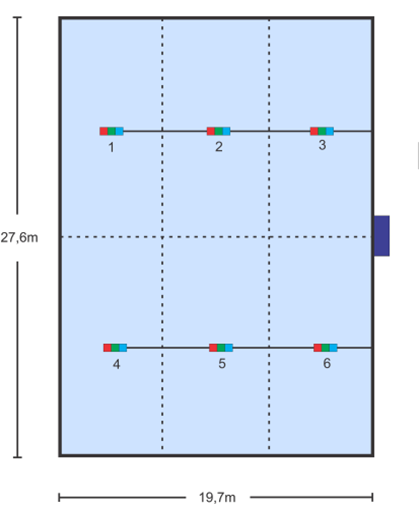
\includegraphics[width=6.5cm,height=3.6cm]{Images/bandoao.png}
		\caption[Thiết kế bản đồ cảm biến ao\cite{zaini2020data}]{\bfseries \fontsize{12pt}{0pt}\selectfont Thiết kế bản đồ cảm biến ao \cite{zaini2020data}}
		\label{bandoao}
	\end{figure}
	

	Bố trí các cảm biến tại 6 góc ao, mỗi góc gồm 3 cảm biến: pH ,DO, nhiệt độ.
	Bên cạnh đó nhóm tác giả đưa ra những phép đo kiểm tra độ chính xác của các cảm biến:
	
	\begin{itemize}
		\item Đối với cảm biến pH DFRobot
		
		Thu thập dữ liệu từ cảm biến pH, thí nghiệm được tiến hành đo dữ liệu của từng mẫu chất lỏng với pH khác nhau và mỗi mẫu được đo trong 10 giây trong Hình \ref{ktPH}.
		\begin{figure}[!ht]
			\centering
			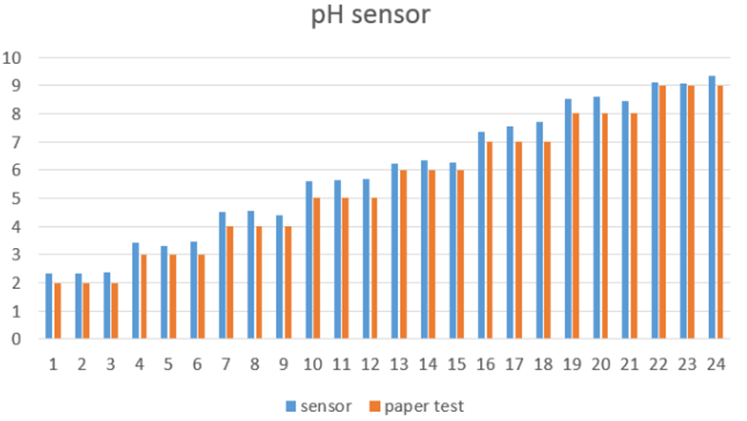
\includegraphics[width=7cm,height=4cm]{Images/ktPH.png}
			\caption[Biểu đồ so sánh cảm biến pH và máy đo \cite{zaini2020data}]{\bfseries \fontsize{12pt}{0pt}\selectfont Biểu đồ so sánh cảm biến pH và máy đo\cite{zaini2020data}}
			\label{ktPH}
		\end{figure}   
		
		Đồ thị so sánh dữ liệu đo từ cảm biến và dụng cụ test. Cho thấy giá trị đọc từ cảm biến (màu xanh) với dụng cụ test (màu cam) không có quá mình khác biệt.
		\item Đối với cảm biến DO
		
		Thử nghiệm được thực hiện sử dụng ba loại dung dịch khác nhau, gồm nước hồ, nước khoáng và nước có ga (nước giải khát). Sử dụng cảm biến DO để kiểm tra mức độ oxy trong ba dung dịch này được thực hiện xen kẽ xem trên Hình \ref{ktDo}.
		
		\begin{figure}[!ht]
			\centering
			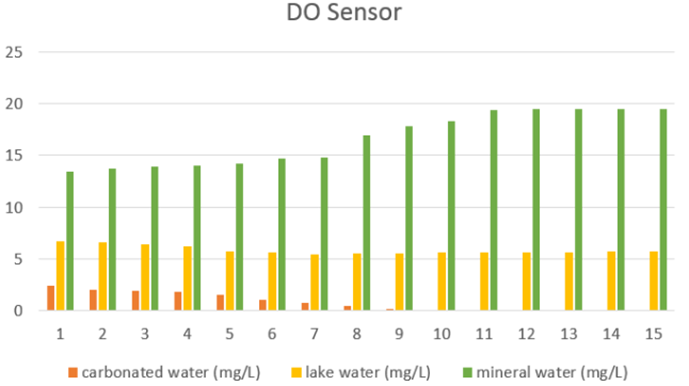
\includegraphics[width=7cm,height=4cm]{Images/ktDo.png}
			\caption[Biểu đồ so sánh cảm biến DO và máy đo \cite{zaini2020data}]{\bfseries \fontsize{12pt}{0pt}\selectfont Biểu đồ so sánh cảm biến DO và máy đo\cite{zaini2020data}}
			\label{ktDo}
		\end{figure}  
		
		Tôm có thể sống khi mức oxy > 4.0 mg/L. Từ các thử nghiệm được thực hiện như trong Hình \ref{ktDo}, có thể thấy tôm sẽ sống sót trong nước hồ (thanh màu vàng) vì có giá trị > 4.0 mg/L. Trong nước có ga (thanh màu đỏ), giá trị DO là 0 mg/L, có thể đảm bảo rằng tôm không thể sống trong nước này vì không thể hít thở được.
		\item Ảnh hưởng của chiều dài cáp
		
		Cảm biến hãng DFRobot có chiều dài khá lớn, càng dài cáp sử dụng, kháng điện càng lớn. Kháng điện quá lớn sẽ ảnh hưởng đến các giá trị đọc của cảm biến vì đây là dữ liệu tương tự. Từ đó bài báo thực nghiệm, kiểm tra tính chính xác của dữ liệu với 2 đoạn dây là 1m và 9m thử nghiệm này có thể thấy được tầm ảnh hưởng của độ dài cáp đối với kết quả của các giá trị đọc của cảm biến.
		\begin{figure}[!ht]
			\centering
			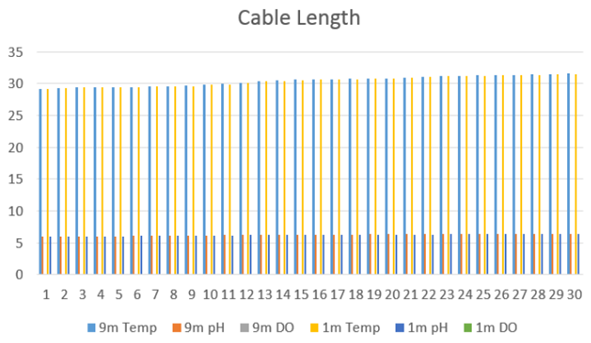
\includegraphics[width=7cm,height=4cm]{Images/ktcap.png}
			\caption[Biểu đồ thanh kiểm tra chiều dài cáp\cite{zaini2020data}]{\bfseries \fontsize{12pt}{0pt}\selectfont Biểu đồ thanh kiểm tra chiều dài cáp\cite{zaini2020data}}
			\label{ktcap}
		\end{figure}  
	\end{itemize}
	
	Dựa trên Hình \ref{ktcap}, có thể thấy sự khác biệt về giá trị đọc của cảm biến giữa thanh màu vàng (9 mét) và thanh màu xanh (1 mét). Nhóm nghiên cứu thu được giá trị độ chính xác là 99.90461\% cho cảm biến pH \cite{zaini2020data}. 
	
	\paragraph{Hệ thống các nút cảm biến phục vụ môi trường nuôi tôm}\mbox{}
	
	Nghiên cứu \cite{khanhhe} hướng đến việc xây dựng một hệ thống có khả năng đo lường và giám sát ảnh hưởng của các thông số môi trường trong ao nuôi tôm công nghiệp (pH, nhiệt độ, nồng độ oxy hòa tan và NH3) trong suốt quá trình nuôi. Hệ thống gồm các nút cảm biến được đặt cố định trong ao nuôi nhằm thu thập các thông số môi trường. Các dữ liệu thu thập được từ các nút này được đồng bộ về một hệ  thống trung tâm, tại đây hệ thống tiếp  tục đồng bộ lên một máy chủ điện toán đám mây. Mỗi ao nuôi sẽ được trang bị một hệ thống riêng và phân biệt bằng một mã định danh, các dữ liệu môi trường được giám sát thông qua một ứng dụng trực tuyến thể hiện trong Hình \ref{TQht}.
	\begin{figure}[!ht]
		\centering
		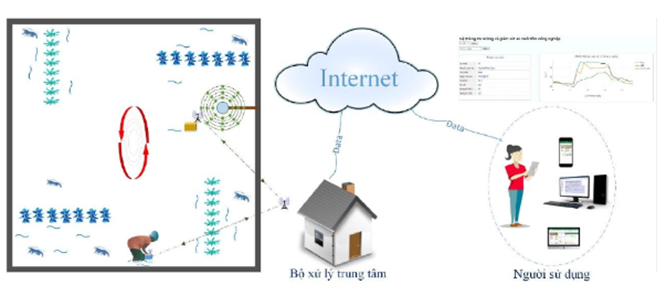
\includegraphics[width=7.5cm,height=4.5cm]{Images/TQht.png}
		\caption[Tổng quan hệ thống \cite{khanhhe}]{\bfseries \fontsize{12pt}{0pt}\selectfont Tổng quan hệ thống\cite{khanhhe}}
		\label{TQht}
	\end{figure}  
	
	\begin{itemize}
		\item Nút cảm biến
		
		Nút cảm  biến được thiết kế thành hai loại: nút cảm biến cố định và nút cảm biến di động. Sơ đồ bố trí các nút cảm biến như Hình \ref{sddulieu}:
		\begin{figure}[!ht]
			\centering
			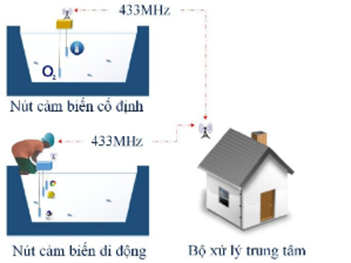
\includegraphics[width=7.8cm,height=4.3cm]{Images/sddulieu.png}
			\caption[Sơ đồ thu thập dữ liệu\cite{khanhhe}]{\bfseries \fontsize{12pt}{0pt}\selectfont Sơ đồ thu thập dữ liệu\cite{khanhhe}}
			\label{sddulieu}
		\end{figure}
		\begin{itemize}[label=$\ast$]
			\item Đối với nút cảm biến cố định
			
			Nút này được đặt cố định tại một vị trí trong ao nuôi để thu thập trực tiếp các thông  số môi trường (nồng độ oxy, nhiệt độ). Số lượng nút cảm biến cố định thay đổi tùy theo diện tích ao nuôi, thường thì được đặt gần vị trí máy cho ăn hoặc hệ thống quạt oxy vì đây là nơi tôm tập trung nhiều nhất. Sơ đồ khối của nút cảm biến cố định như Hình \ref{nutcodinh}.
			
			\begin{figure}[!ht]
				\centering
				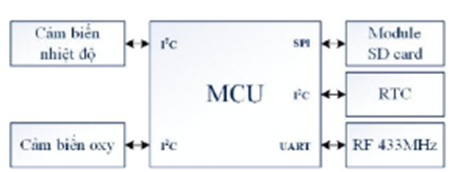
\includegraphics[width=6cm,height=3cm]{Images/nutcodinh.png}
				\caption[Sơ đồ khối nút cảm biến cố định\cite{khanhhe}]{\bfseries \fontsize{12pt}{0pt}\selectfont Sơ đồ khối nút cảm biến cố định\cite{khanhhe}}
				\label{nutcodinh}
			\end{figure}
			
			Từ Hình \ref{nutcodinh} thấy dữ liệu thu thập từ các cảm biến sẽ được mã hóa và truyền về bộ  trung tâm qua kết nối  không dây sử dụng tần số sóng mang 433MHz. 
			
			
			\item Đối với nút cảm biến di động
			
			Có vai trò thu tập các thông số (pH, nhiệt độ) và tính cơ động cao từ đó đo được nhiều ao, tiết kiệm được chi phí. Dữ liệu cũng được mã hóa và truyền về bộ trung tâm qua kết nối khống dây. Cấu trúc của nút cảm biến này như Hình \ref{nutdidong}
			\begin{figure}[!ht]
				\centering
				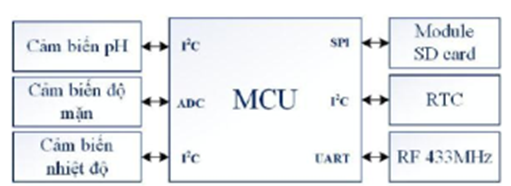
\includegraphics[width=7cm,height=3cm]{Images/nutdidong.png}
				\caption[Sơ đồ khối nút cảm biến di định\cite{khanhhe}]{\bfseries \fontsize{12pt}{0pt}\selectfont Sơ đồ khối nút cảm biến di định\cite{khanhhe}}
				\label{nutdidong}
			\end{figure}
		\end{itemize}
		\item Thiết bị trung tâm
		
		\begin{figure}[!ht]
			\centering
			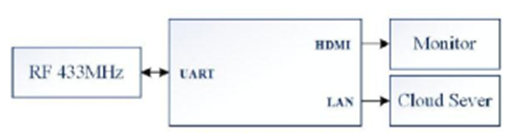
\includegraphics[width=6.5cm,height=2cm]{Images/tbtrungtam.png}
			\caption[Sơ đồ khối bộ xử lý trung tâm\cite{khanhhe}]{\bfseries \fontsize{12pt}{0pt}\selectfont Sơ đồ khối bộ xử lý trung tâm\cite{khanhhe}}
			\label{tbtrungtam}
		\end{figure}
		    
		Bộ xử lý trung tâm giữ vai trò là trung tâm thu thập dữ liệu từ tất cả các nút cảm biến, đồng bộ dữ liệu về máy chủ điện toán đám mây. Dữ liệu này được truy xuất bởi một ứng dụng trực tuyến nhằm phục vụ việc giám sát và đánh giá. Cấu trúc của bộ xử lý trung tâm như Hình \ref{tbtrungtam}.
		
		Việc thu thập dữ liệu từ các nút cảm biến được kiểu kết hơp giữa kiểu hình sao và hỏi vòng nhằm tăng khoảng cách truyền  và nhận dữ  liệu. Các thành phần  của hệ thống có thể nằm ở các vùng như minh họa trong Hình \ref{sdtdl}.
		
		\begin{figure}[!ht]
			\centering
			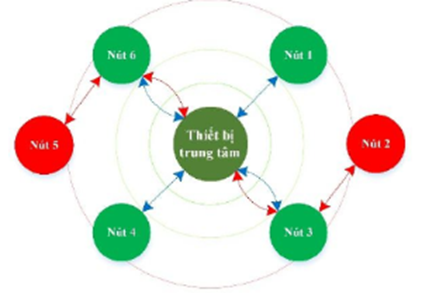
\includegraphics[width=5.5cm,height=4cm]{Images/sdtdl.png}
			\caption[Sơ đồ truyền nhận dữ liệu\cite{khanhhe}]{\bfseries \fontsize{12pt}{0pt}\selectfont Sơ đồ truyền nhận dữ liệu\cite{khanhhe}}
			\label{sdtdl}
		\end{figure} 
		
		Thiết bị trung tâm gửi tín hiệu yêu cầu cập nhật dữ liệu theo thứ tự đến các nút cảm biến. Khi các nút cảm biến nhận được tín hiệu từ thiết bị trung tâm sẽ truyền dữ liệu về tuần  tự theo yêu cầu của thiết bị trung tâm. Trong trường hợp thiết bị trung tâm bị mất kết nối một hoặc nhiều nút thì thiết bị trung tâm ghi nhận lại nút bị mất và chuyển sang nút khác để lấy dữ liệu cho đến nút cuối cùng.    
	\end{itemize}
	
	
	\subsubsection{Công nghệ truyền thông trong IOT}
	
	\paragraph{Công nghệ mạng không dây sử dụng trong IOT}\mbox{}
	
	Có nhiều công nghệ không dây có thể được sử dụng cho các mạng cảm biến không dây. Các công nghệ phổ biến với động lực thị trường tốt về mặt đối tác lớn, triển khai và hồ sơ quan hệ công chúng (PR) được đánh giá là Bluetooth, ZigBee, Wi-Fi, GSM, Sigfox và LoRa.
	
	\begin{table}[H]
		\centering
		\begin{tabular}{|l|l|l|l|l|l|}
			\hline
			\begin{tabular}[c]{@{}l@{}}Công nghệ \\ không dây\end{tabular} & \begin{tabular}[c]{@{}l@{}}Tần số \\ hoạt động\end{tabular}       & Phạm vi                                              & \begin{tabular}[c]{@{}l@{}}Tốc độ \\ dữ liệu\end{tabular}    & \begin{tabular}[c]{@{}l@{}}Sử dụng\\  năng lượng\end{tabular} & \begin{tabular}[c]{@{}l@{}}Cấu trúc \\ liên kết\end{tabular} \\ \hline
			Bluetooth                                                      & 2.4 Ghz                                                           & 100m                                                 & 1 Mbps                                                       & 10 - 500 mW                                                   & điểm - điểm                                                  \\ \hline
			Zigbee                                                         & 2.4 Ghz                                                           & 300m                                                 & 250 kbps                                                     & 1 mW                                                          & lưới                                                         \\ \hline
			Wifi                                                           & \begin{tabular}[c]{@{}l@{}}2.4 , 3.6, 5 \\ và 60 GHz\end{tabular} & 150m                                                 & \begin{tabular}[c]{@{}l@{}}6 Mbps \\ -6.75 Gbps\end{tabular} & 1 W                                                           & sao                                                     \\ \hline
			GSM                                                            & \begin{tabular}[c]{@{}l@{}}700 -\\ 2600 MHz\end{tabular}          & \begin{tabular}[c]{@{}l@{}}10 -\\ 30 km\end{tabular} & \begin{tabular}[c]{@{}l@{}}35 Kbps -\\ 1 Gbps\end{tabular}   & 1 - 5 W                                                       &  sao                                                     \\ \hline
			Sigfox                                                         & 868 MHz                                                           & 20- 50 km                                            & 100 bps                                                      & 160 mW                                                        &  sao                                                     \\ \hline
			Lora                                                           & 433,868 MHz                                                       & 10 -30 km                                            & 0.3 -5.5 kbps                                                & 100 mW                                                        &  sao, lưới                                               \\ \hline
		\end{tabular}
		\caption[Sự khác biệt của các công nghê không dây \cite{shuda2018towards}]{\bfseries\fontsize{12pt}{0pt}\selectfont Sự khác biệt của các công nghê không dây \cite{shuda2018towards}}
		\label{wireless}
	\end{table}
	
	Bảng \ref{wireless} trình bày tóm tắt các công nghệ không dây khác nhau được đánh giá theo phạm vi, tốc độ dữ liệu, sử dụng năng lượng và cấu trúc liên kết mạng. Bluetooth, ZigBee và Wi-Fi không có đủ phạm vi để triển khai trên một nhà máy điện mặt trời quy mô tiện ích. GSM sử dụng quá nhiều năng lượng khi truyền và không có vùng phủ sóng GSM trên hầu hết các nhà máy điện mặt trời nằm ở Nam Phi. Sigfox là một LPWAN (Mạng Khu Vực Rộng Công Suất Thấp) với phạm vi dài nhưng tốc độ dữ liệu không đủ để gửi dữ liệu đo lường theo các khoảng thời gian đều đặn. Sigfox chỉ cho phép gửi một thông điệp 12-byte mỗi 10 phút.
	
	Công nghệ không dây được chọn cho WSN đề xuất là LoRa. LoRa được chọn vì phạm vi dài, tiêu thụ năng lượng thấp và tốc độ dữ liệu đủ. LoRa là một công nghệ điều chế không dây, nó là lớp vật lý để kết nối với các nút khác hoặc một cổng. LoRa sử dụng kỹ thuật điều chế phổ lan truyền dựa trên chirp. Nó chống nhiễu, đa đường và suy giảm do kỹ thuật điều chế độc đáo của nó. LoRa có băng thông thấp và sử dụng rất ít năng lượng. Nó hoạt động trong các băng tần ISM không giấy phép trên khắp thế giới, 433 MHz và 868 MHz ở Nam Phi. Các chipset radio LoRa sử dụng tối đa 100 mW khi truyền. Các module LoRa có phạm vi từ 10 km đến 30 km ở các khu vực ngoại ô.
	
	LoRa sử dụng các yếu tố trải rộng khác nhau (SF) thiết lập tốc độ điều chế, do đó cũng ảnh hưởng đến tốc độ dữ liệu. Phạm vi SF từ SF7 đến SF12. SF7 là nhanh nhất (5,5 kbps ở 868 MHz) nhưng không có phạm vi rất dài trong khi SF12 là chậm nhất (300 bps ở 868 MHz) nhưng nó có phạm vi rất dài, như được thấy trong Hình \ref{SFlora}.
	
	\begin{figure}[!ht]
		\centering
		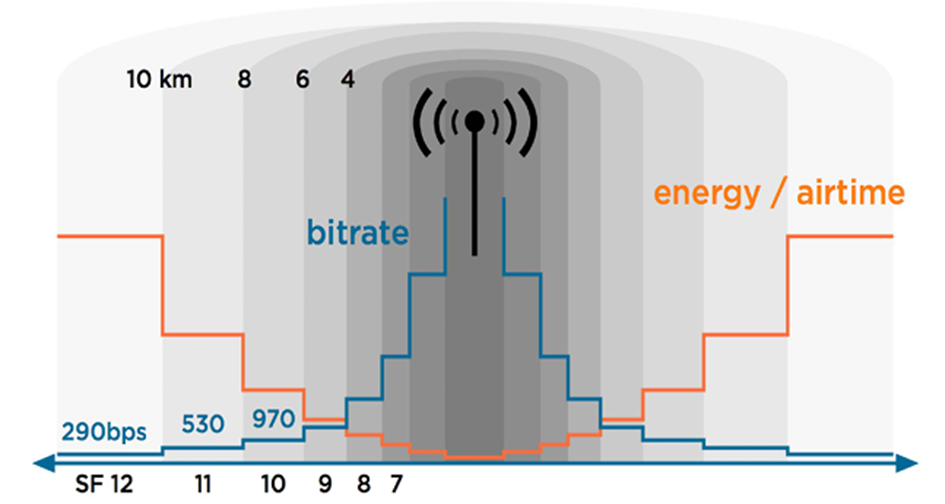
\includegraphics[width=7cm,height=4cm]{Images/SFlora.png}
		\caption[Hệ số lan truyền LoRa, tốc độ bit và thời gian truyền\cite{LoRaAlliance}]{\bfseries \fontsize{12pt}{0pt}\selectfont Hệ số lan truyền LoRa, tốc độ bit và thời gian truyền \cite{LoRaAlliance}}
		\label{SFlora}
	\end{figure}
	
	Trong bài báo, tác giả\cite{shuda2018towards} sử dụng hệ số trải rộng là 12 và băng thông là 125 KHz và kiểm tra phạm vi đã được thực hiện và đạt được phạm vi 9,27 km.
	
	
	\newpage
	\paragraph{Giao thức LoRaWAN}\mbox{}
	
	LoRaWAN là một giao thức MAC, được xây dựng để sử dụng tầng vật lý LoRa. Nó được thiết kế chủ yếu cho các mạng cảm biến, trong đó các cảm biến trao đổi các gói tin với máy chủ với tốc độ dữ liệu thấp và khoảng thời gian tương đối dài (một lần truyền mỗi giờ hoặc thậm chí mỗi ngày). Phần này mô tả đặc tả LoRaWAN V1.0 \cite{LoRaAlliance}, được phát hành vào tháng 1 năm 2015.
	
	\begin{itemize}
		\item Các thành phần của mạng LoRaWAN : 
		Nhiều thành phần của mạng được định nghĩa trong đặc tả LoRaWAN và cần thiết để hình thành một mạng LoRaWAN: các thiết bị đầu cuối, các cổng (tức là các trạm cơ sở) và máy chủ mạng.
		
		\begin{itemize}[label=$\ast$]
			\item Thiết bị đầu cuối (End-device): Là các cảm biến tiêu thụ điện năng thấp giao tiếp với các cổng bằng cách sử dụng LoRa.
			\item Cổng (Gateway): Là các thiết bị trung gian chuyển tiếp các gói tin đến từ các thiết bị đầu cuối đến máy chủ mạng qua một giao diện IP backhaul cho phép thông lượng lớn hơn, chẳng hạn như Ethernet hoặc 3G. Có thể có nhiều cổng trong một triển khai LoRa, và cùng một gói dữ liệu có thể được nhận (và chuyển tiếp) bởi nhiều cổng.
			\item Máy chủ mạng (Network server): Chịu trách nhiệm loại bỏ các bản sao và giải mã các gói tin do các thiết bị gửi và tạo ra các gói tin cần được gửi lại cho các thiết bị.
		\end{itemize}
		
		Không giống như các mạng di động truyền thống, các thiết bị đầu cuối không được liên kết với một cổng cụ thể để truy cập vào mạng. Các cổng chỉ đơn giản phục vụ như một liên kết chuyển tiếp lớp và chuyển tiếp gói tin nhận từ các thiết bị đầu cuối đến máy chủ mạng sau khi thêm thông tin về chất lượng tiếp nhận. Do đó, một thiết bị đầu cuối được liên kết với một máy chủ mạng, máy chủ này chịu trách nhiệm phát hiện các gói tin trùng lặp, chọn cổng thích hợp để gửi trả lời (nếu có), và do đó gửi lại các gói tin đến các thiết bị đầu cuối. Về mặt logic, các cổng là trong suốt đối với các thiết bị đầu cuối.
		
		\item LoRaWAN có ba lớp thiết bị đầu cuối khác nhau để đáp ứng các nhu cầu khác nhau của ứng dụng:
		
		\begin{itemize}[label=$\ast$]
			\item Class A, hai chiều: Thiết bị đầu cuối Class A có thể lên lịch truyền tải dựa trên nhu cầu của chúng, với một độ trễ ngẫu nhiên (biến đổi ngẫu nhiên trước khi truyền tải). Lớp này cho phép truyền thông hai chiều, trong đó mỗi lần truyền tải sẽ được theo sau bởi hai khoảng thời gian nhận dữ liệu ngắn. Truyền tải từ máy chủ vào bất kỳ thời điểm nào khác phải chờ đến khi lần truyền tải tiếp theo xảy ra. Thiết bị Class A có mức tiêu thụ năng lượng thấp nhất nhưng cũng cung cấp ít linh hoạt hơn trong việc truyền tải ngược chiều.
			\item Class B, hai chiều với các khe nhận theo lịch trình: Thiết bị đầu cuối Class B mở các cửa sổ nhận bổ sung vào các thời điểm theo lịch trình. Một tín hiệu đồng bộ từ cổng là cần thiết để máy chủ mạng biết khi nào thiết bị đầu cuối đang nghe.
			\item Class C, hai chiều với khe nhận tối đa: Thiết bị đầu cuối Class C có cửa sổ nhận gần như liên tục, do đó có mức tiêu thụ năng lượng tối đa.
		\end{itemize}
		
		LoRaWAN quy định rằng mạng LoRaWAN nên sử dụng các băng tần ISM. Các băng tần này chịu sự điều chỉnh về công suất truyền tải tối đa và chu kỳ hoạt động. Các giới hạn chu kỳ hoạt động này dẫn đến các khoảng trễ giữa các khung truyền tải liên tiếp của thiết bị. Nếu giới hạn là 1\%, thiết bị sẽ phải chờ 100 lần thời gian của khung cuối cùng trước khi truyền lại trên cùng một kênh.
		
		\item Cấu trúc bản tin của LoraWan.
		
		\begin{itemize}[label=$\ast$]
			\item LoRaWAN sử dụng định dạng khung vật lý như mô tả trong Phần 3.3. Header và CRC là bắt buộc đối với các tin nhắn uplink, điều này làm cho việc sử dụng hệ số lan rộng là sáu trong LoRaWAN không thể thực hiện được. Các tin nhắn downlink có header, nhưng không có CRC. Tỷ lệ mã hóa cần phải sử dụng không được chỉ định và cũng không rõ khi thiết bị cuối nên sử dụng tối ưu hóa tốc độ dữ liệu thấp.
			
			\item Định dạng bản tin được chi tiết trong Hình \ref{khungdulieu} DevAddr là địa chỉ ngắn của thiết bị. FPort là trường cổng đa năng. Giá trị không nghĩa là gói tin chứa chỉ các lệnh MAC. Khi điều này xảy ra, trường FOptsLen phải là không. FCnt là bộ đếm khung. MIC là mã code bảo mật, được tính toán trên các trường MHDR, FHDR, FPort và FRMPayload đã mã hóa. MType là loại tin nhắn, cho biết, ngoài việc đó là uplink hoặc downlink tin nhắn và liệu đó là một tin nhắn xác nhận hay không. Sự chấp nhận được yêu cầu cho các tin nhắn xác nhận. Major là phiên bản LoRaWAN; hiện tại, chỉ một giá trị của không là hợp lệ. ADR và ADRAckReq điều khiển cơ chế điều chỉnh tốc độ dữ liệu bởi máy chủ mạng. 
			
		\end{itemize}
		\begin{figure}[!ht]
			\centering
			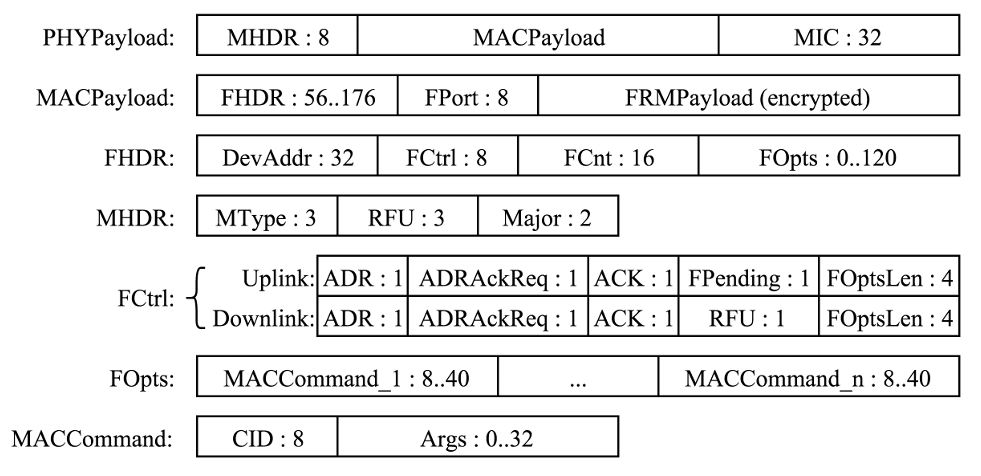
\includegraphics[width=9cm,height=4.5cm]{Images/khungdulieu.png}
			\caption[Định dạng bản tin của LoraWan \cite{augustin2016study}]{\bfseries \fontsize{12pt}{0pt}\selectfont Định dạng bản tin của LoraWan \cite{augustin2016study}}
			\label{khungdulieu}
		\end{figure}
		
		\item Tổng dung lượng kênh và tải kênh
		
		\begin{itemize}[label=$\ast$]
			\item Tổng Dung Lượng: Đây là tổng khả năng truyền dữ liệu tích lũy trên tất cả các kênh logic trong mạng. Mỗi kênh logic được xác định bởi một sự kết hợp cụ thể của dải tần số và hệ số lan rộng. Tổng dung lượng của mạng là tổng của các dung lượng của tất cả các kênh logic này. Ví dụ, trong một dải tần số 125 kHz, với sáu hệ số lan rộng khả dụng (SF7 đến SF12), tổng dung lượng của một kênh 125 kHz có thể lên đến 12,025 bit mỗi giây (bps).
			
			\item Tải Kênh: Tải kênh đại diện cho mức độ sử dụng của dung lượng có sẵn trên một kênh logic tại bất kỳ thời điểm nào. Nó được xác định bởi các yếu tố như số lượng thiết bị LoRa đang cố gắng gửi dữ liệu, tốc độ truyền của chúng và các hệ số lan rộng được sử dụng. Một tải kênh cao hơn cho thấy sự sử dụng lớn hơn của dung lượng của kênh đó. Trong điều kiện tối ưu, một tải kênh bằng một có nghĩa là kênh đã bão hòa với các truyền dữ liệu.
		\end{itemize}
		
		\item Ước tính tỷ lệ va chạm
		
		\begin{itemize}[label=$\ast$]
			
			\item Không có cơ chế nghe trước khi nói (listen-before-talk) hoặc CSMA (Carrier Sense Multiple Access). Điều này làm cho LoRaWAN rất giống với ALOHA, nhưng khác ALOHA ở chỗ có độ dài gói tin thay đổi.
			
			\item Độ dài biến đổi của các gói tin không ảnh hưởng lớn đến hiệu suất của LoRaWAN, và khi tất cả đã xong, hành vi quan sát được rất gần với ALOHA thuần túy. Sử dụng tối đa dung lượng đạt 18\% dung lượng kênh và đạt được cho tải liên kết là 0,48. Tuy nhiên, ở tải này, khoảng 60\% các gói tin được truyền bị loại bỏ do va chạm.Tất cả được minh họa ở Hình \ref{collision}:
			\begin{figure}[!ht]
				\centering
				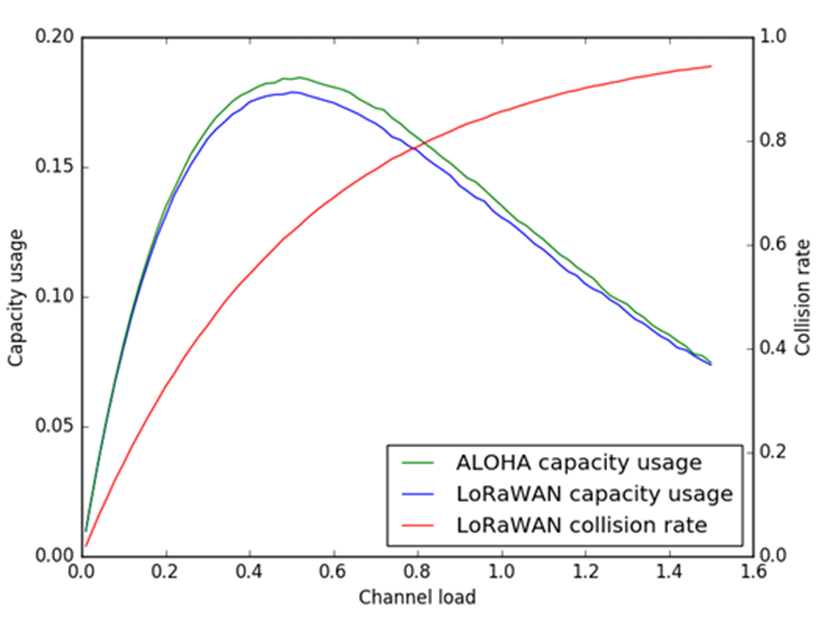
\includegraphics[width=7cm,height=4cm]{Images/collision.png}
				\caption[xung đột gói trong mạng LoRaWAN \cite{augustin2016study}]{\bfseries \fontsize{12pt}{0pt}\selectfont xung đột gói trong mạng LoRaWAN \cite{augustin2016study}}
				\label{collision}
			\end{figure}    
		\end{itemize}
		
		
	\end{itemize}
	
	\paragraph{Công suất tiêu thụ của công nghệ Lora và Giao thức LoraWan}\mbox{}
	
	Mức độ tiêu thụ dòng đối với bộ phát và bộ thu sử dụng Semtech SX1276/77/78/79 LoRa với điều kiện nguồn đầu vào là 3.3V nhiệt độ là 25 \textdegree C, và tần số  hoạt động là 868MHz.
	
	Đối với bộ phát ta có Hình \ref{table2}:
	
	\begin{figure}[!ht]
		\centering
		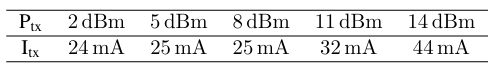
\includegraphics[width=8.5cm,height=1.5cm]{Images/table2.png}
		\caption[Dòng sử dụng của bộ phát tương ứng với các công suất phát\cite{ochoa2017evaluating}]{\bfseries \fontsize{12pt}{0pt}\selectfont Dòng sử dụng của bộ phát tương ứng với các công suất phát \cite{ochoa2017evaluating}}
		\label{table2}
	\end{figure}
	
	Đối với bộ thu ta có Hình \ref{table3}:
	\begin{figure}[!ht]
		\centering
		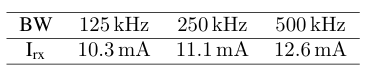
\includegraphics[width=6cm,height=1.5cm]{Images/table3.png}
		\caption[Dòng sử dụng của bộ thu tương ứng với các BW khác nhau \cite{ochoa2017evaluating}]{\bfseries \fontsize{12pt}{0pt}\selectfont Dòng sử dụng của bộ thu tương ứng với các BW khác nhau \cite{ochoa2017evaluating}}
		\label{table3}
	\end{figure}
	
	Trong bài báo\cite{ochoa2017evaluating}, tác giả đã đề cập tới mức tiêu thụ năng lượng để truyền một gói tin bằng các cấu hình mạng khác nhau trong nội dung này em đề cấp đến mức tiêu thụ năng lượng của giao thức LoRaWAN được sử dụng trong cấu trúc Star Topology. 
	
	Đầu tiên,tác giả đề cập tới mức tiêu thụ năng lượng phụ thuộc vào các thông số như hệ số trải phổ và công suất truyền được minh họa trong Hình \ref{125lost}.
	
	\begin{figure}[!ht]
		\centering
		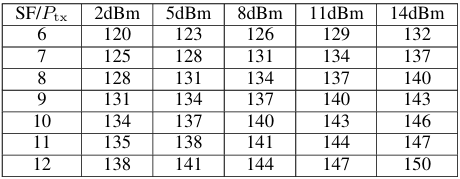
\includegraphics[width=7cm,height=3.5cm]{Images/125lost.png}
		\caption[Mất mát liên kết(MCL) tối đa của LoRa với băng thông 125kHz\cite{ochoa2017evaluating}]{\bfseries \fontsize{12pt}{0pt}\selectfont Mất mát liên kết(MCL) tối đa của LoRa với băng thông 125kHz\cite{ochoa2017evaluating}}
		\label{125lost}
	\end{figure}
	
	"Maximum Coupling Loss" (MCL) là mức độ mất mát tín hiệu tối đa cho phép giữa hai thiết bị truyền thông (thường là giữa máy phát và máy thu) mà vẫn đảm bảo việc truyền thông tin hiệu quả.
	\newpage
	Mức tiêu thụ năng lượng cho cấu trúc Star Topology sẽ được tính bằng\cite{ochoa2017evaluating}:
	\begin{equation}
		E_{\mathrm{star}\left(S F, P_{\mathrm{tx}}\right)}=  E_{\mathrm{tx}}+E_{\mathrm{rx}}    
	\end{equation}
	
	Trong đó:
	\begin{itemize}
		\item $E_{\mathrm{tx}}$ : mức tiêu thụ của phía phát.
		\item $E_{\mathrm{rx}}$ : mức tiêu thụ của phía thu.
	\end{itemize}
	
	Thời gian phát sóng của một gói $t_{\mathrm{packet}}$ phụ thuộc vào SF, BW và CR.Theo đó, mức tiêu thụ năng lượng cho cấu trúc Star Topology có thể được diễn đạt như sau\cite{ochoa2017evaluating}:
	\begin{equation}
		E_{\mathrm{star}\left(S F, P_{\mathrm{tx}}\right)}=t_{\mathrm{packet}} \cdot\left(P_{\mathrm{tx}}+P_{\mathrm{rx}}\right) \\
		=\frac{L_{\mathrm{packet}}}{R_{\mathrm{b}}} \cdot\left(P_{\mathrm{tx}}+P_{\mathrm{rx}}\right) \\    
	\end{equation}
	
	Trong đó:
	\begin{itemize}
		\item $L_{\mathrm{packet}}$ :kích thước của gói được truyền tính bằng bit.
		\item $P_{\mathrm{rx}}$ :Công suất phía thu.
		\item $P_{\mathrm{tx}}$ :Công suất máy phát.
	\end{itemize}
	
	\begin{figure}[!ht]
		\centering
		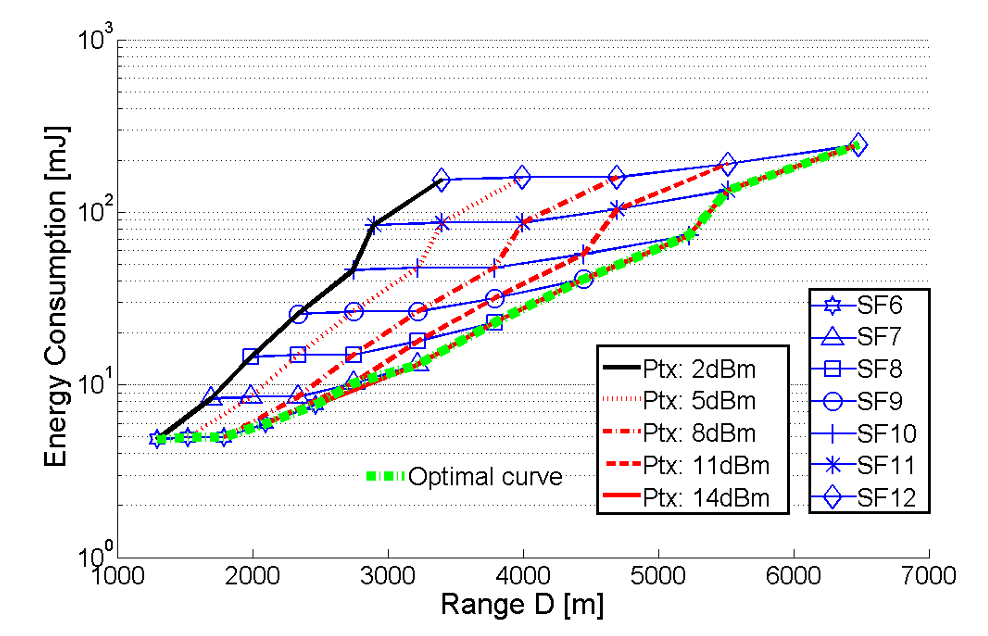
\includegraphics[width=9cm,height=5cm]{Images/tieuthu125.png}
		\caption[Tiêu thụ năng lượng  ở BW 125kHz - $\mathrm{CR}=\frac{4}{5}$ theo phạm vi truyền D\cite{ochoa2017evaluating}]
		{\bfseries \fontsize{12pt}{0pt}\selectfont Tiêu thụ năng lượng  ở BW 125kHz -  $\mathrm{CR}=\frac{4}{5}$ theo phạm vi truyền D\cite{ochoa2017evaluating}}
		\label{tieuthu125}
	\end{figure}
	
	Hình \ref{tieuthu125} cho thấy mức tiêu thụ năng lượng như một hàm số của phạm vi khoảng cách truyền cho các giá trị khác nhau của (SF, $P_{\mathrm{tx}}$). Khi tăng $P_{\mathrm{tx}}$ (đường cong màu xanh), tiêu thụ năng lượng trơn tru sự gia tăng tion được quan sát thấy đối với SF cố định. Khi chuyển đổi SF tăng dần với $P_{\mathrm{tx}}$ cố định (đường cong màu đỏ), năng lượng tiêu dùng tăng nhanh hơn. Vì vậy, nó thích hợp hơn cho tăng phạm vi, đầu tiên là tăng $P_{\mathrm{tx}}$ và sau đó là tăng cường hệ số lan truyền.
	
	\begin{figure}[!ht]
		\centering
		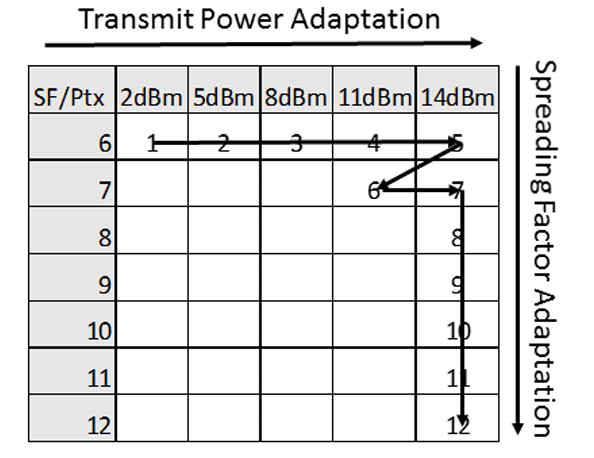
\includegraphics[width=7cm,height=4cm]{Images/chienluoccs.png}
		\caption[Tối ưu mức tiêu thụ ở BW 125kHz\cite{ochoa2017evaluating}]
		{\bfseries \fontsize{12pt}{0pt}\selectfont Tối ưu mức tiêu thụ ở BW 125kHz\cite{ochoa2017evaluating}}
		\label{chienluoccs}
	\end{figure}
	
	Hình \ref{chienluoccs} tác giả đã đưa ra các nghiên cứu lựa chọn các thông số phù hợp liên quan đến SF và $P_{\mathrm{tx}}$ để Lora có mức tiêu thụ năng lượng thấp nhất.
	
	Tiếp theo,tác giả đề cập tới mức tiêu thụ năng lượng phụ thuộc và băng thông sử dụng.Tác giả phân tích mức tiêu thụ năng lượng theo ba giá trị băng thông: 125kHz, 250kHz và 500kHz.Thực hiện giống với bằng thông 125kHz cho băng thông 250kHz và 500kHz và kết quả thu được được minh họa ở Hình \ref{tieuthuall}:
	
	\begin{figure}[!ht]
		\centering
		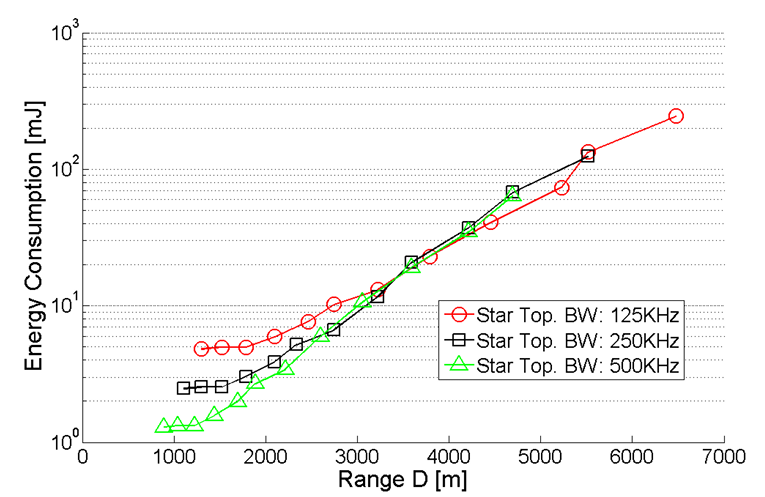
\includegraphics[width=9cm,height=5cm]{Images/tieuthuall.png}
		\caption[Tối ưu mức tiêu thụ ở các BW khác nhau\cite{ochoa2017evaluating}]
		{\bfseries \fontsize{12pt}{0pt}\selectfont Tối ưu mức tiêu thụ ở các BW khác nhau \cite{ochoa2017evaluating}}
		\label{tieuthuall}
	\end{figure}
	
	Tác giả cho rằng phạm vi tối đa tăng lên khi BW giảm. Điều này là do MCL cao hơn với mức thấp hơn BW. Tuy nhiên, BW thấp đi kèm với thông lượng thấp hơn và do đó, thời gian phát sóng dài hơn, dẫn đến giá trị cao hơn tiêu thụ năng lượng. Theo đó, đối với khoảng cách D < 2.6km, sử dụng BW = 500kHz cho phép tiêu thụ năng lượng thấp hơn sự tiêu thụ. Ngoài khoảng cách D = 2.6km, tiêu thụ năng lượng tương tự cho ba giá trị băng thông. Sau đó, BW sự thích ứng không có tác động đáng kể đến năng lượng.
	
	Từ các nghiên cứu trên tác giả đã đưa ra chiến lược tối ưu mức tiêu thu cho các 
	BW khác nhau với công suất truyền và hệ số trải phổ khác nhau trong Hình \ref{toiuuallBW}:
	
	\begin{figure}[!ht]
		\centering
		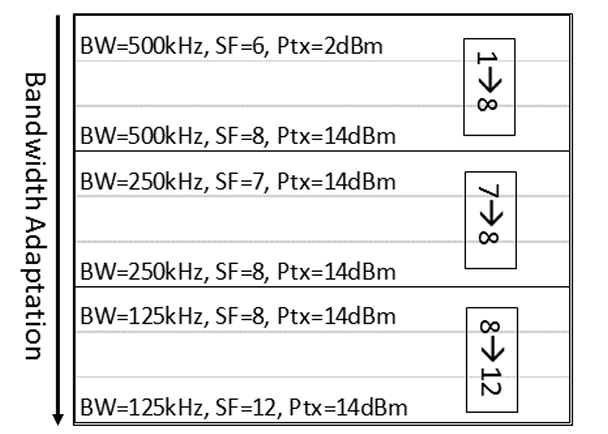
\includegraphics[width=7cm,height=3.9cm]{Images/toiuuallBW.png}
		\caption[Chiến lược tối ưu mức tiêu thụ ở các BW khác nhau \cite{ochoa2017evaluating}]
		{\bfseries \fontsize{12pt}{0pt}\selectfont Chiến lược tối ưu mức tiêu thụ ở các BW khác nhau \cite{ochoa2017evaluating}}
		\label{toiuuallBW}
	\end{figure}
	
	Cấu hình tiêu thụ năng lượng thấp nhất là (BW = 500kHz, SF6, Ptx = 2dBm). Đối với BW =500kHz, hộp ở bên phải (1–>8) đề cập đến cách thức tối ưu mức tiêu thụ trong Hình \ref{chienluoccs} Do đó, các thức tối ưu tốt nhất vẫn là điều chỉnh công suất truyền tải đầu tiên (lên đến Ptx = 14dBm) và sau đó, điều chỉnh độ trải rộng hệ số (lên tới SF8). Sau đó, các thức tối ưu đó được áp dụng cho băng thông 250kHz và 125kHz theo vào các hộp.
	
	\subsection{Phương pháp đề xuất cho hệ thống}
	
	Từ việc tham khảo và khảo sát các bài báo nghiên cứu, em xin đề xuất đề tài \textbf{“Mô hình mạng cảm biến không dây quan trắc môi trường nước trong nuôi tôm chân trắng”}. Em sẽ thiết kế hệ thống gồm 2 nút cảm biến, 1 thiết bị trung tâm. Nút cảm biến tích hợp pin mặt trời đồng thời sử dụng pin và lưới điện, có tích hợp truyền thông không dây là lora và sim, có thể hiển thị thông số qua LCD, lưu trữ thông qua thẻ SD. Thiết bị trung tâm sẽ nhận tín hiệu từ nút cảm biến thông qua lora và gửi dữ liệulên server thông qua sim. Dữ liệu sẽ được theo dõi trên GIS
	
	\subsection{Kết luận}
	
	CHƯƠNG 1 tập trung nghiên cứu tổng quan về tình hình nuôi tôm hiện nay tại Việt Nam, bên cạnh cơ hội là những khó khăn, và rủi ro gặp phải trong quá trình nuôi tôm, các nghiên cứu liên quan đã được công bố. Thông qua quá trình tìm hiểu, em đã nắm bắt được cơ bản về cách thức hoạt động và mô hình hóa hệ thống. Thông qua quá trình khảo sát các bài báo, em đã đề xuất đề tài cho bài toán xây dựng hệ thống cảm biến không dây theo dõi môi trường nuôi tôm. Tuy đề xuất vẫn còn thiếu sót không thể tránh khỏi nhưng cũng đã hoạt động tương đối tốt và ổn định, đã được thử nghiệm trong thời gian dài. Tới chương sau, em sẽ trình bày về cơ sở lý thuyết tổng quan bao gồm cả những phần được sử dụng trong đồ án này.
    
	
	\newpage
	%% CHAPTER 2 
	\section*{CHƯƠNG 2.  CƠ SỞ LÝ THUYẾT}
	\addcontentsline{toc}{section}{\numberline{}CHƯƠNG 2.  CƠ SỞ LÝ THUYẾT}
	\setcounter{section}{2}
    \setcounter{subsection}{0}
	\setcounter{figure}{0}
	\setcounter{table}{0}
	
	Sau khi nghiên cứu và tìm hiểu và đề xuất hệ thống ở CHƯƠNG 1. Chương này sẽ chủ yếu tìm hiểu các cơ sở kiến thức cần thiết liên quan tới quá trình phát triển và thực hiện đề tài.
	
	
	\subsection{Các thông số chỉ tiêu trong môi trường nuôi tôm}
	
	Chất lượng nước đóng vai trò vô cùng quan trọng và có tác động đáng kể tới việc nuôi thủy sản, đặc biệt là việc nuôi tôm. Chất lượng nước ảnh hưởng trực tiếp đến hiệu quả của thức ăn, tốc độ sinh trưởng và tỉ lệ sống của tôm. Nếu môi trường nước không đảm bảo, tôm có thể đối diện với các vấn đề như suy giảm số lượng, bệnh tật, tốc độ sinh trưởng chậm và hiệu quả sử dụng thức ăn giảm đi. Vấn đề nguồn nước luôn được người nuôi tôm đặt lên hàng đầu và luôn cẩn thận trong quá trình xử lý nước để đưa và nuôi tôm để đảm bảo tôm phát triển bình thường và khỏe mạnh, nước phải được duy trì sạch sẽ và không bị ô nhiễm.
	
	Chất lượng nước phụ thuộc vào nhiều yếu tố như chất lượng nguồn nước, chất đất, cách thức cho ăn, điều kiện thời tiết, công nghệ nuôi và chế độ quản lý đầm nuôi. Để đánh giá chất lượng nước, người nuôi cần theo dõi và kiểm tra liên tục nhiều thông số sinh học, hóa học và lý tưởng khác nhau. Việc này giúp người nuôi có thể phát hiện vấn đề và xử lý nước kịp thời để bảo vệ sự phát triển và sức khỏe của tôm trong quá trình nuôi trồng.
	
	Theo QCVN 02 - 19 : 2014/BNNPTNT do Tổng cục Thủy sản biên soạn và trình ban hành; Bộ Nông nghiệp và Phát triển nông thôn ban hành kèm theo Thông tư số 22/2014/TT-BNNPTNT ngày 29 tháng 7 năm 2014 \cite{Thuysanta}, chất lượng nước cấp vào ao để nuôi tôm chân trắng và tôm sú được trình bày Bảng \ref{bang21}.
	
	Trong Bảng \ref{bang21}, có thể thấy có rất nhiều yếu tố quyết định đến chất lượng môi trường nuôi tôm. Tuy nhiên với đề tài này, em chọn 4 thông số quan trọng ảnh hưởng lớn tới sự phát triển của tôm bao gồm: nhiệt độ, pH, DO và độ mặn.
	
	\begin{table}[H]
		\centering
		\begin{tabular}{|l|l|l|l|}
			\hline
			\textbf{Thông số} & \textbf{Đơn vị} & \textbf{Giá trị cho phép}                                                   & \textbf{Giá trị hợp lý} \\ \hline
			Ôxy hoà tan (DO)  & mg/l            & $\geq 3.5$                                                                 & $\geq 5$              \\\hline
			pH 7 ÷ 9          &                 & \begin{tabular}[c]{@{}l@{}}Dao động trong ngày \\ không quá 0,5\end{tabular} & 7.5 ÷ 8.5               \\ \hline
			Độ mặn            & \%o             & 5 ÷ 35                                                                      & 10 ÷ 25                 \\ \hline
			Độ kiềm           & mg/l            & 60 ÷ 180                                                                    &                         \\ \hline
			Độ trong          & cm              & 20 ÷ 50                                                                     & 30 ÷ 35                 \\ \hline
			$NH_3$               & mg/l            & $< 0.03$                                                                  &                         \\ \hline
			$H_2S$               & mg/l            & $<0.05$                                                                 &                         \\ \hline
			Nhiệt độ          & \textdegree C              & 18 ÷ 33                                                                     & 20 ÷ 30                 \\ \hline
		\end{tabular}
		\caption[Bảng thông số chất lượng nước nuôi tôm ]{\bfseries\fontsize{12pt}{0pt}\selectfont Bảng thông số chất lượng nước nuôi tôm }
		\label{bang21}
	\end{table}
	
	Sau đây sẽ là sự ảnh hưởng của 4 thông số nhiệt độ, pH, DO và độ mặn môi trường nuôi tôm.
	
	\subsubsection{ Sự ảnh hưởng của nhiệt độ tới môi trường nuôi tôm}
	
	Nhiệt độ là yếu tố có khả năng tác động mạnh mẽ đến sức khỏe của tôm. Khi nhiệt độ thay đổi nhanh chóng, tôm dễ bị sốc nhiệt và suy yếu dần. Đây cũng là một trong những nguyên nhân gây ra dịch bệnh ở tôm, đặc biệt khi nhiệt độ cao có thể dẫn đến hiện tượng chết hàng loạt, gây tổn thất nặng nề cho người nuôi.
	Không chỉ vậy, nhiệt độ cao làm tôm thay đổi thân nhiệt theo môi trường sống, dẫn đến quá trình trao đổi chất diễn ra liên tục khiến chúng ăn nhiều hơn. Tuy nhiên, do lượng men tiêu hóa trong cơ thể tôm có hạn, việc này không chỉ khó hấp thụ dinh dưỡng mà còn làm tăng chi phí nuôi nhưng hiệu quả lại không cao.
	Theo nghiên cứu \cite{ambio}, nếu nhiệt độ ao nuôi là 30\textdegree C thì lượng thức ăn tôm tiêu thụ cao hơn khoảng 36,5\% so với nhiệt độ 29\textdegree C, nhưng tốc độ tăng trưởng của tôm ở hai mức nhiệt độ này là như nhau. Tuy nhiên, tỷ lệ sống của tôm ở nhiệt độ 33\textdegree C thấp hơn so với 29\textdegree C vì chất lượng nước suy giảm. 
	Vì thế, nhiệt độ lý tưởng cho quá trình sống và sinh sản của tôm nên dao động từ 20-30 \textdegree C.
	
	\subsubsection{ Sự ảnh hưởng của DO tới môi trường nuôi tôm}
	
	Oxy chính là yếu tố giúp duy trì sự sống và oxy hòa tan chính là dưỡng khí cần thiết cho sự hô hấp và phát triển của các loài sinh vật dưới nước không chỉ riêng tôm. Tuy ở mỗi một giai đoạn, nhu cầu DO của tôm không giống nhau. Theo \cite{DO}, nồng độ oxy hòa tan thấp có thể khiến cá và tôm bị căng thẳng, dễ nhiễm bệnh, tăng trưởng chậm và giảm ăn, dẫn đến dư thừa thức ăn trong ao, tăng hệ số chuyển hóa thức ăn (FCR), và tích tụ khí độc gây ô nhiễm môi trường nước. Ngoài ra, DO thấp có thể thay đổi cộng đồng vi sinh vật dưới nước, gia tăng vi khuẩn có hại và giảm lợi khuẩn. Ngược lại, mức DO quá cao có thể làm tăng trưởng sinh vật khó kiểm soát và gây ra hiện tượng tảo nở hoa. Vì phụ thuộc vào các yếu tố như: sức khỏe, khả năng hấp thụ của từng cá thể…Nếu lượng DO ít hơn 5 mg/l sẽ dẫn đến hiện tượng ăn ít ở tôm, tăng trưởng chậm, ảnh hưởng đến quá trình lột xác. Nếu tình trạng kéo dài sẽ tôm sẽ dễ mắc các bệnh nguy hiểm khác cũng như chết tôm.
	
	\subsubsection{ Sự ảnh hưởng của PH tới môi trường nuôi tôm}
	
	Theo \cite{NuoiTom} pH của nước ao nuôi tôm ảnh hưởng đáng kể đến hệ sinh thái ao và sức khỏe tôm. Khi pH quá cao (mang tính bazơ), nước thường trong, khó gây màu và thủy sinh vật đáy phát triển mạnh, dẫn đến biến động pH trong ngày rất lớn. Nguồn nước này không phù hợp để nuôi tôm và cần hạ pH xuống mức 7,5-8. Ngược lại, pH quá thấp (mang tính axit) cũng ảnh hưởng đến tảo và vi sinh vật trong nước, có thể do nước bị nhiễm phèn, sụp tảo và quá trình phân hủy vật chất hữu cơ. Sự phát triển mạnh của tảo quang hợp gây ra dao động pH lớn, cho thấy môi trường bị phú dưỡng và thành phần loài tảo thay đổi theo chiều hướng không tốt, như sự xuất hiện của tảo lam với pH rất cao.
	
	pH vượt ngưỡng ảnh hưởng bất lợi đến sức khỏe tôm, làm tôm chậm lột vỏ, suy giảm miễn dịch và stress. Sự mất cân bằng áp suất thẩm thấu và pH thấp trong giai đoạn tôm lột vỏ có thể gây hiện tượng tôm dính chân không lột được vỏ. Biến đổi pH ảnh hưởng đến quá trình tiêu hóa của tôm, làm chúng còi cọc, không lớn và suy giảm hệ miễn dịch, dễ nhiễm bệnh. Ngoài ra, pH cao làm tăng nồng độ khí độc $NH_3$, trong khi pH thấp làm bùng phát khí độc $H_2S$, cả hai đều cực kỳ nguy hiểm và ảnh hưởng nghiêm trọng đến tôm nuôi. Sự suy giảm khả năng trao đổi khí ở mang, làm tôm ngạt và nổi đầu, và quá trình trao đổi chất bị gián đoạn cũng là những tác động tiêu cực từ biến đổi pH.
	
	\subsubsection{ Sự ảnh hưởng của độ mặn tới môi trường nuôi tôm}
	
	Độ mặn của muối ảnh hưởng đến sự tồn tại, phát triển và duy trì chức năng sinh lý của tôm thông qua quá trình điều hòa áp suất thẩm thấu cũng như tăng khả năng kháng khuẩn và miễn dịch ở tôm. Tuy nhiên, cần kiểm soát độ mặn một cách nghiêm ngặt. Bởi vì: Nếu độ mặn quá thấp các icon $Ca^{2+}, Mg^{2+}, Na^{+}$… trong nước với hàm lượng thấp làm cho quá trình lột xác của tôm diễn ra không đồng đều, tôm bị mềm vỏ sau khi lột làm tăng tỉ lệ hao hụt gấp nhiều lần dẫn đến tôm bị suy giảm chức năng đề kháng. Ngược lại, nếu sống trong môi trường có độ mặn cao, Trên mức chịu đựng, tôm sẽ còi cọc, chậm lớn, Thậm chí là sốc và chết hàng loạt. Hơn nữa, khi độ mặn tăng cao, bệnh phân trắng và hoại tử gan tụy cấp tính sẽ diễn biến hết sức phức tạp, gây nên dịch bệnh làm thiệt hại rất lớn về mặt kinh tế. 
	
	
	\subsection{Lý thuyết về các thông số và cảm biến}
	\subsubsection{Lý thuyết PH}
	
	pH là một chỉ số đo nồng độ ion hydroxonium \( \text{H}_3\text{O}^+ \) trong dung dịch. Đây là một thang đo định tính để xác định tính axit hay bazơ của một chất lỏng. Giá trị pH thường dao động từ $0$ đến $14$ với công thức tính phụ thuộc vào nồng độ 2 ion \( \text{OH}^- \) và \( \text{H}^+ \) trong dung dịch như sau: 
	
	\begin{equation}
		\mathrm{pH}=\log \frac{[H+]}{[O H-]} \\    
	\end{equation}
	
	Nếu $pH < 7$ , thì dung dịch được xem là axit, trong đó $pH = 0$ đại diện cho axit mạnh nhất và pH gần 7 đại diện cho axit yếu. Nếu $pH = 7$, thì dung dịch được coi là trung tính, chẳng hạn như nước tinh khiết. Trong khi đó, nếu 
	$pH > 7$, thì dung dịch được xem là bazơ, trong đó $pH = 14$ đại diện cho bazơ mạnh nhất và pH gần 7 đại diện cho bazơ yếu.
	
    Điều này cho phép chúng ta xác định mức độ axit hoặc bazơ của một chất và cũng rất hữu ích trong các quá trình hóa học, sinh học, và các lĩnh vực khác trong cuộc sống hàng ngày. Để đo pH, chúng ta thường sử dụng các chỉ thị pH hoặc máy đo pH. 	
	
	\paragraph{Cảm biến pH}\mbox{}
	
	Cảm biến pH hay còn gọi là đầu dò pH có chức năng chuyển đổi giá trị pH thành các giá trị điện áp tương ứng.
	
	Thông thường để đo độ pH của dung dịch là sử dụng giấy quỳ tím. Nó chuyển sang màu khác tùy thuộc vào biểu đồ pH mà không xét đến hàm lượng ion hydro, tuy nhiên, máy đo pH phải sử dụng đầu dò pH để đo nồng độ ion hydro. 
	
	Đầu dò pH thủy tinh là một điện cực chọn lọc ion (ISE – Ion selective electrode). Hệ thống đo lường này về cơ bản bao gồm ISE phản ứng với một loại ion đặc biệt, trong trường hợp này là ion H+ và một điện cực tham chiếu được nhúng chung vào mẫu cần đo. Cảm biến ISE hydro được cung cấp một thế điện hóa học bị ảnh hưởng bởi hoạt tính của ion hydro trong dung dịch. Tuy nhiên, điện cực tham chiếu được thiết kế để tạo ra một thế điện hóa học không phụ thuộc vào thành phần của mẫu. Sự khác biệt giữa hai điện thế này, cụ thể là điện áp (mV) được hiển thị trên bộ đo pH, xác định giá trị pH dựa trên phương trình Nernst: 
	
	\begin{equation}
		\mathrm{E}=E_0-\frac{R T}{n F} \ln \left(\frac{C_1}{C_2}\right)     
	\end{equation}
	
	
	Trong đó :
	\begin{itemize}
		\item E: Điện thế điện cực của dung dịch cần đo (đơn vị: V)
		\item $E_0$: Điện thế điện cực tham chiếu (đơn vị: V)
		\item R :Hằng số Boltzmann $8.31439 \text{J mol}^{-1} \text{K}^{-1}$
		\item T: Nhiệt độ (đơn vị K)
		\item $C_1$, $C_2$: Nồng độ ion \( \text{H}^+ \) ở trong dung dịch 1 và 2
	\end{itemize}

Điện cực/hệ thống tham chiếu và hydro ISE (tức là điện cực có màng thủy tinh) có thể là các điện cực riêng biệt Hình \ref{ISE}.	

	\begin{figure}[!ht]
		\centering
		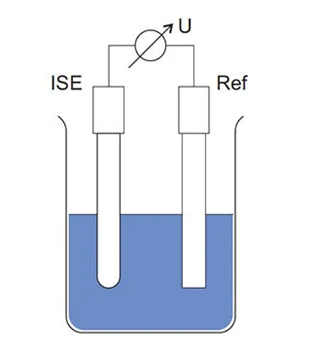
\includegraphics[width=5cm,height=5.5cm]{Images/ISE.png}
		\caption[Sơ đồ cấu trúc của ISE hydro, tham chiếu và vôn kế \cite{HeadPH}]{\bfseries \fontsize{12pt}{0pt}\selectfont Sơ đồ cấu trúc của ISE hydro, tham chiếu và vôn kế \cite{HeadPH}}
		\label{ISE}
	\end{figure}
	
	Hình \ref{PH} mô tả về cấu tạo của đầu dò pH với đầu cực thủy tinh để xác định điện thế tác động bởi ion \( \text{H}^+ \) trong dung dịch, bên trong cảm biến là dung dịch mẫu KCl có chức năng tạo mức điện thế mẫu. Hiệu điện thế khi đo được xác định bằng hiệu điện thế của 2 thanh kim loại AgCl.
	
	\begin{figure}[!ht]
		\centering
		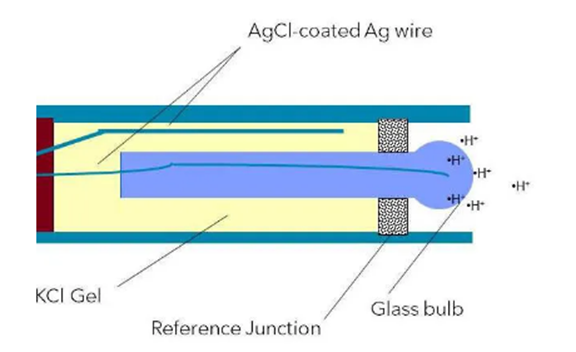
\includegraphics[width=6cm,height=5.3cm]{Images/PHhead.png}
		\caption[Sơ đồ cấu trúc của ISE hydro, tham chiếu và vôn kế \cite{HeadPH}]{\bfseries \fontsize{12pt}{0pt}\selectfont Sơ đồ cấu trúc của ISE hydro, tham chiếu và vôn kế\cite{HeadPH}}
		\label{PH}
	\end{figure}

	\subsubsection{Lý thuyết chung về Oxi hòa tan và cảm biến DO }
	\paragraph{Lý thuyết chung về Oxi hòa tan}\mbox{}
	
	Oxy hòa tan (sau đây viết tắt là DO) là oxy $O_2$ hòa tan trong nước, và trong thế giới tự nhiên, nó được hòa tan trong nước theo tỷ lệ với áp suất riêng phần của $O_2$ trong khí quyển. Mức oxy hòa tan được biểu thị bằng lượng $O_2$ hòa tan trên một đơn vị thể tích nước $(\text{mg/L})$. Oxy đi vào nước bằng cách hấp thụ trực tiếp từ khí quyển, do chuyển động nhanh hoặc dưới dạng chất thải của quá trình quang hợp của thực vật. Nhiệt độ nước và khối lượng nước di chuyển có thể ảnh hưởng đến mức oxy hòa tan. Dưới đây là các công thức tính khối lượng Oxy bão hòa trong nước (Phương trình Weiss):
	
	\begin{equation}
		{[\mathrm{DO}]=D O_0 * F_S * F_P}     
	\end{equation}
	
	\begin{equation}
		\begin{split}
			\mathrm{DO}_0&=1.4295 \exp \left[-173.4292+249.6339\left(\frac{100}{\mathrm{T}}\right)\right. \\
			&\qquad\left.+143.3483\left(\ln \frac{\mathrm{T}}{100}\right)-21.8492\left(\frac{\mathrm{T}}{100}\right)\right]
		\end{split}
	\end{equation}
	
	\begin{equation}
		F_S=\exp \left\{S *\left[-0.033096+0.014259\left(\frac{T}{100}\right)-0.0017\left(\frac{T}{100}\right)^2\right]\right\} \\  
	\end{equation}
	\begin{equation}
		F_P=\frac{P-u}{760-u} v \text { ới } u=10^{\left(8.10765-\frac{1750.286}{235+t}\right)} \\  
	\end{equation}
	
	
	\begin{itemize}
		\item DO: Nồng độ oxi bão hòa 100\% thực tế tại môi trường đo [mg/l] 
		\item $DO_0$: Nồng độ oxi bão hòa 100\% trong nước ngọt [mg/l] 
		\item $F_s$: Hệ số hiệu chỉnh độ mặn 
		\item $F_p$: Hệ số hiệu chỉnh áp suất 
		\item t : Nhiệt độ của nước [ \textdegree C ] 
		\item T: Nhiệt độ của nước [Kelvin] T= 273.15 + t 
		\item u:  áp suất hơi nước 
		\item P áp suất không khí [mmHg]    
	\end{itemize}
	
	\paragraph{Cảm biến đo DO }\mbox{}
	
	Đầu dò oxy hòa tan hoạt động bằng cách đo lượng oxy khuếch tán qua màng thấm (hoặc bán thấm) vào đầu dò (cảm biến). Khi oxy đi vào cảm biến, phản ứng khử hóa học xảy ra, tạo ra tín hiệu điện.
	
	\begin{figure}[!ht]
		\centering
		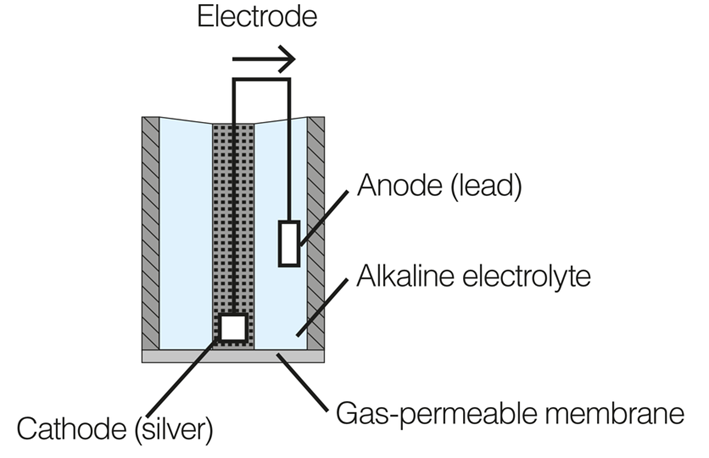
\includegraphics[width=8cm,height=5.8cm]{Images/DO.png}
		\caption[Sơ đồ cấu tạo đầu đo DO loại Galvanic\cite{LAQUA}]{\bfseries \fontsize{12pt}{0pt}\selectfont Sơ đồ cấu tạo đầu đo DO loại Galvanic\cite{LAQUA}}
		\label{DO}
	\end{figure}
	
	Cấu trúc của đầu đo oxy (DO) điện phân giống như được mô tả trong Hình \ref{DO}. Điểm đặc biệt chính của nó chính là sự xuất hiện của một lớp màng lọc ion đặc biệt, có khả năng chọn lọc, chỉ cho phép các ion oxy ($O_2$) thông qua và không cho phép các ion khác. Nguyên tắc này giúp đảm bảo sự chính xác và đáng tin cậy của quá trình đo lường.
	
	Để thực hiện đo lường, đầu đo được đặt trong một buồng điện phân kiềm được chứa trong dung dịch kiềm như KOH, NaOH. Các điện cực trong đầu đo được làm từ hai loại kim loại khác nhau: điện cực anot làm bằng chì (Pb), trong khi điện cực catôt được tạo từ một thanh bạc. 
	
	Đặc biệt, điện cực catôt được đặt sát với lớp màng thẩm thấu oxy. Khi oxy tan trong nước kiểm tra, nó sẽ thẩm thấu qua lớp màng thẩm thấu đặc biệt được làm từ vật liệu như Teflon hoặc polyethylen. Quá trình thẩm thấu này cho phép lượng oxy cần đo lường được chuyển tiếp và ghi nhận một cách chính xác và nhanh chóng.
	
	Khi cảm biến DO điện phân được ngâm trong mẫu nước, oxy thẩm thấu qua màng thẩm thấu oxy, tỷ lệ thuận với áp suất của oxy trong nước, rồi bị khử và tiêu thụ tại cực catôt. Phản ứng này tạo ra một dòng điện điện tử trực tiếp liên quan đến nồng độ oxy. Dòng điện này được mang bởi các ion trong dung dịch điện phân và chạy từ cực catôt đến cực anot.
	
	\begin{equation}
		\text{Cực anot (Pb) - phản ứng oxi hóa chì:} \quad 2\text{Pb} \rightarrow 2\text{Pb}^{2+} + 4e^-
	\end{equation}
	\begin{equation}
		\text{Cực catốt (Ag) - phản ứng khử oxy:} \quad \text{O}_2 + 4e^- + 2\text{H}_2\text{O} \rightarrow 4\text{OH}^-
	\end{equation}
	\begin{equation}
		\text{Phản ứng tổng hợp:} \quad \text{O}_2 + 2\text{H}_2\text{O} + 2\text{Pb} \rightarrow 2\text{Pb(OH)}_2
	\end{equation}
	
	Dòng điện được tạo ra tỉ lệ thuận với lượng oxy tiêu thụ và do đó tỉ lệ thuận với áp suất riêng của oxy trong mẫu. Do vậy lượng oxy tham gia vào quá trình phản ứng sẽ tỷ lệ với lượng Oxy thẩm thấu qua lớp màng thẩm thấu.
	
	\subsubsection{Lý thuyết chung về độ mặn và cảm biến EC}
	\paragraph{Lý thuyết chung về độ mặn }\mbox{}
	
	Độ mặn là một đặc trưng quan trọng trong các loại dung dịch hay môi trường nước. Nó thường được đo bằng nồng độ các ion muối có trong mẫu nước. Độ mặn thể hiện số lượng muối hòa tan trong một đơn vị thể tích của nước hoặc khối lượng của nước.
	
	Đơn vị của độ mặn là \text{\permil} (phần nghìn), tuy nhiên đây không phải là đơn vị đo của đơn vị nồng độ (g/kg) của các muối hòa tan trong nước biển.
	
	Các phạm vi độ mặn của nước dựa trên S\permil:
	\begin{itemize}
		\item Nước ngọt: \( S\permil = 0.02 - 0.5 \) ppt.
		\item Nước lợ: \( S\permil = 0.5 - 16 \) ppt.
		\item Nước mặn: \( S\permil = 16 - 47 \) ppt.
		\item Nước quá mặn: \( S\permil > 47 \) ppt.
	\end{itemize}
	
	Vể sau, A.F.Karpevits đã bổ sung và chi tiết như sau:
	\begin{itemize}
		\item Nước ngọt: 0,01 – 0,5ppt (các sông hồ, hồ chứa). 
		\item Nước ngọt nhạt: 0,01 – 0,2ppt. 
		\item Nước ngọt lợ: 0,2 – 0,5ppt. 
		\item Nước lợ: 0,5 - 30ppt (các hồ, biển nội địa, cửa sông).
		\item Nước lợ nhạt: 0,5 - 4ppt.
		\item Nước lợ vừa: 4 - 18ppt. 
		\item Nước lợ mặn: 18 - 30ppt
		\item Nước biển: 30 - 40ppt (Đại dương, biển hở, biển nội địa, vịnh vũng, cửa sông). 
		\item Nước quá mặn: 40 - 300ppt (một số hồ, vịnh, vũng)
	\end{itemize}
	Mối quan hệ giữa độ mặn và độ dẫn:
	Công thức liên hệ giữa độ mặn, độ dẫn và nhiệt độ như sau\cite{islam2023iot} :
	\begin{equation}
		\text { Salinity }=\mathrm{a}_0+\mathrm{r}_2\left(\mathrm{a}_1+\mathrm{r}_2\left(\mathrm{a}_2+\mathrm{r}_2\left(\mathrm{a}_3+\mathrm{r}_2\left(\mathrm{a}_4+\mathrm{r}_2 \mathrm{a}_5\right)\right)\right)\right)+\mathrm{ds}    
	\end{equation}
	
	
	Trong đó : 
	\begin{itemize}
		\item $r=\frac{E C}{42914}$
		\item $\mathrm{r}_2=\sqrt{r}$
		\item $\mathrm{ds}=\mathrm{b}_0+\mathrm{r}_2\left(\mathrm{~b}_1+\mathrm{r}_2\left(\mathrm{~b}_2+\mathrm{r}_2\left(\mathrm{~b}_3+\mathrm{r}_2\left(\mathrm{~b}_4+\mathrm{r}_2 \mathrm{~b}_5\right)\right)\right)\right) \times \frac{t e m p-15.0}{1.0+0.0162(t e m p-15.0)}$
	\end{itemize}
	
	Các hệ số đặc trưng cho tính toán độ mặn dựa trên việc hiệu chuẩn độ dẫn:
	\[
	\begin{aligned}
		a_0 &= 0.008, & a_1 &= -0.1692, & a_2 &= 25.3851, \\
		a_3 &= 14.0941, & a_4 &= -7.0261, & a_5 &= 2.7081, \\
		b_0 &= 0.0005, & b_1 &= -0.0056, & b_2 &= -0.0066, \\
		b_3 &= -0.0375, & b_4 &= 0.0636, & b_5 &= -0.0144, \\
		c_0 &= 0.6766097, & c_1 &= 0.0200564, & c_2 &= 0.0001104259, \\
		c_3 &= -0.00000069698, & c_4 &= 0.0000000010031
	\end{aligned}
	\]
	\paragraph{Cảm biến đo EC }\mbox{}
	
	Cảm biến EC đo độ dẫn điện hoạt động dựa trên nguyên tắc đo khả năng dẫn điện của dung dịch có thể đạt bằng cách dùng điện cực bằng bạch kim (một tế bào 2 điện cực), một điện áp được áp dụng vào hai tấm phẳng ngâm trong dung dịch, và dòng điện chạy qua dung dịch giữa hai điện cực được đo, sau đó đo độ dẫn điện G, có thể được tính toán bằng cách sử dụng định luật Ohm nghịch đảo. 
	
	\begin{equation}
		R = \frac{V}{I}, \quad G = \frac{1}{R}    
	\end{equation}
	
	Trong đó: 
	R là điện trở, V  là điện áp giữa 2 cực và I là dòng điện.
	\begin{figure}[!ht]
		\centering
		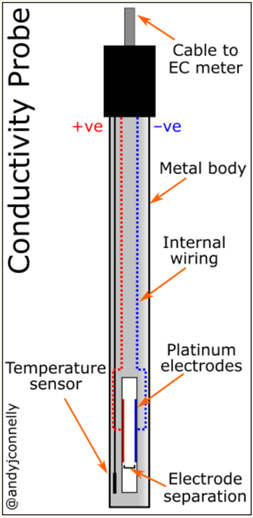
\includegraphics[width=3cm,height=7cm]{Images/EC.png}
		\caption[Sơ đồ đầu đo dẫn điện\cite{EC}]{\bfseries \fontsize{12pt}{0pt}\selectfont Sơ đồ đầu đo dẫn điện\cite{EC}}
		\label{EC}
	\end{figure}
	
	Cấu trúc đầu đo độ dẫn điện (EC) giống như được mô tả trong Hình \ref{EC} Việc thiết lập một đầu dò độ dẫn điện cơ bản với hai điện cực bạch kim vuông. Thiết kế cụ thể của đầu dò sẽ thay đổi tùy thuộc vào phạm vi độ dẫn điện cần đo. Diện tích của các điện cực và khoảng cách giữa chúng xác định phạm vi này. Các giá trị này được gói gọn trong hằng số tế bào (K).
	Hằng số tế bào (K) được xác định là tỷ lệ giữa khoảng cách giữa các điện cực (d) và diện tích điện cực (A). Tuy nhiên, hiệu ứng vùng lề (fringe-field effect - AF) làm thay đổi diện tích điện cực:
	
	\begin{equation}
		K = \frac{d}{A + AF}
	\end{equation}
	
	Đối với các dung dịch có độ dẫn điện thấp, các điện cực có thể được đặt gần nhau hơn hoặc làm lớn hơn để hằng số tế bào nhỏ hơn một. Điều này làm tăng dẫn khí để tạo ra một giá trị dễ dàng hơn để hiểu bằng máy đo. Ngược lại cũng áp dụng, trong các dung dịch có độ dẫn điện cao, các điện cực được đặt xa nhau hơn hoặc làm nhỏ hơn để giảm dẫn khí của mẫu.
	
	Giá trị K lý tưởng cho một cảm biến thay đổi với phạm vi dẫn khí được đo. Thông thường, một tế bào với K = 0.1 (1/cm) được chọn để đo nước tinh khiết, trong khi đối với nước môi trường biển nước lợ các tế bào có K = 10 (1/cm) thích hợp hơn cho các mẫu có độ dẫn điện rất cao.
	
	\begin{figure}[!ht]
		\centering
		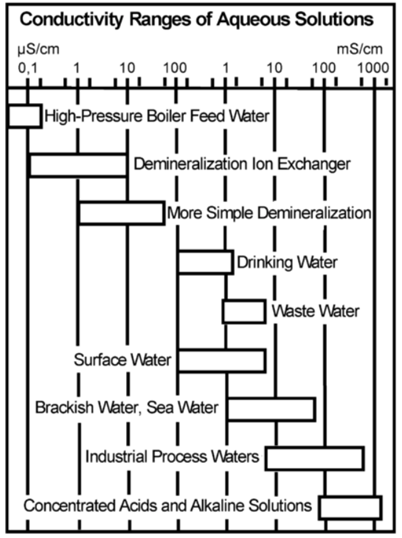
\includegraphics[width=7cm,height=7cm]{Images/dodandien.png}
		\caption[Độ dẫn điện của các dung dịch thông dụng\cite{Conductivity}]{\bfseries \fontsize{12pt}{0pt}\selectfont Độ dẫn điện của các dung dịch thông dụng\cite{Conductivity}}
		\label{dodandien}
	\end{figure}
	
	Hình \ref{dodandien} mô tả phạm vi độ dẫn của dung dịch (electrical conductivity of solutions) với một số loại dung dịch. Quan tâm chính tới nước Suface water – nước bề mặt, Sea water – nước biển,   Một cảm biến dẫn điện cơ bản với hai điện cực bạch kim hình vuông. Thiết kế cụ thể của cảm biến sẽ thay đổi tùy thuộc vào phạm vi dẫn điện cần đo. Diện tích của các điện cực (Hình \ref{ECActivity})và khoảng cách giữa chúng xác định phạm vi này. Các giá trị này được biểu diễn trong hằng số tế bào (K). 
	
	
	Độ dẫn điện C, giữa các điện cực được tính bằng công thức:
	\begin{equation}
		C = \frac{G \cdot d}{A}
	\end{equation}
	
	Trong đó:
	\begin{itemize}
		\item  C : là độ dẫn điện (S/cm).
		\item  G : là dẫn khí (S).
		\item  d : là khoảng cách giữa các điện cực (cm).
		\item  A : là diện tích của các điện cực (${cm}^{2}$).
	\end{itemize}
	
	\begin{figure}[!ht]
		\centering
		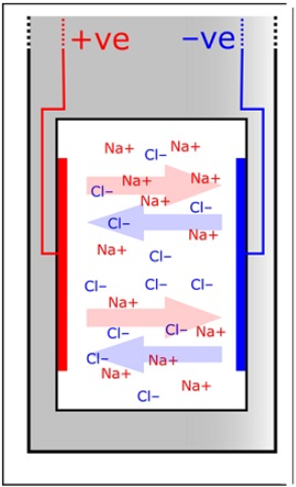
\includegraphics[width=3.7cm,height=7cm]{Images/HD.png}
		\caption[Sơ đồ thể hiện hoạt động của đầu dò độ dẫn điện\cite{EC}]{\bfseries \fontsize{12pt}{0pt}\selectfont Sơ đồ thể hiện hoạt động của đầu dò độ dẫn điện\cite{EC}}
		\label{ECActivity}
	\end{figure}
	
   \newpage
	\subsubsection{Lý thuyết chung về nhiệt độ và cảm biến nhiệt độ }
	\paragraph{Lý thuyết về nhiệt độ và nhiệt độ trong nước }\mbox{}
	
	Nhiệt độ là một khái niệm quan trọng trong vật lý và khoa học tự nhiên, nó đo lường mức độ nóng hay lạnh của một vật thể hoặc môi trường. Nhiệt độ phản ánh mức độ chuyển động của các phân tử, nguyên tử hoặc hạt nhỏ bên trong một vật liệu.
	
	Theo lý thuyết nhiệt độ của vật liệu, khi nhiệt độ tăng lên, các phân tử, nguyên tử hoặc hạt nhỏ trong vật liệu cũng sẽ có chuyển động nhanh hơn, gây ra sự mở rộng và làm nóng vật liệu. Trong trường hợp nhiệt độ giảm xuống, chuyển động của các phân tử cũng chậm lại, làm cho vật liệu co lại và làm lạnh nó. 
	
	Nhiệt độ trong nước là một khía cạnh quan trọng của môi trường nước, đóng vai trò quan trọng trong hệ sinh thái và ảnh hưởng đến sự tồn tại và hoạt động của các sinh vật sống trong nước. Nhiệt độ của nước phụ thuộc vào nhiều yếu tố và có tác động lớn đến sự phân bố và đa dạng của các loài sinh vật trong môi trường nước.
	Các yếu tố chủ yếu ảnh hưởng đến nhiệt độ trong nước gồm:
	
	\begin{itemize}
		\item Ánh sáng mặt trời: Ánh sáng mặt trời chiếu vào môi trường nước, làm nó hấp thụ năng lượng nhiệt và dẫn đến tăng nhiệt độ của nước. Năng lượng từ ánh sáng được hấp thụ dưới dạng nhiệt và làm nước ấm lên.
		\item Địa hình dưới nước: Các yếu tố địa hình dưới nước như sự thay đổi độ sâu, dòng chảy nước, và môi trường bao quanh sẽ ảnh hưởng đến phân bố nhiệt độ trong môi trường nước. Các khu vực nông và có ánh sáng mặt trời trực tiếp thường có nhiệt độ cao hơn so với các khu vực sâu và bóng râm.
		\item Thời tiết: Các yếu tố thời tiết như nhiệt độ môi trường, gió, mưa cũng có ảnh hưởng đến nhiệt độ trong nước.
		\item Độ sâu của nước: Nhiệt độ của nước thường giảm theo độ sâu. Tầng nước bề mặt thường có nhiệt độ cao hơn so với tầng nước ở độ sâu lớn hơn.
		\item Sự hòa tan các chất trong nước: Nước có khả năng hòa tan các chất khác nhau và điều này cũng có thể ảnh hưởng đến nhiệt độ của nước.
	\end{itemize}
	
	\paragraph{Lý thuyết về trở nhiệt và cảm biến nhiệt độ }\mbox{}
	
	Điện trở nhiệt được định nghĩa là một loại điện trở có điện trở thay đổi theo sự thay đổi của nhiệt độ. Mặc dù điện trở của tất cả các điện trở sẽ dao động nhẹ theo nhiệt độ, nhưng điện trở nhiệt đặc biệt nhạy cảm với sự thay đổi nhiệt độ. Do đó giá trị của trở nhiệt (Resistance) sẽ phụ thuộc vào nhiệt độ (Temperature) xung quanh trở nhiệt Hình \ref{pttemp} dưới đây sẽ mô tả chi tiết sự ảnh hưởng của nhiệt độ tới giá trị của trở nhiệt.
	
	
	\begin{figure}[!ht]
		\centering
		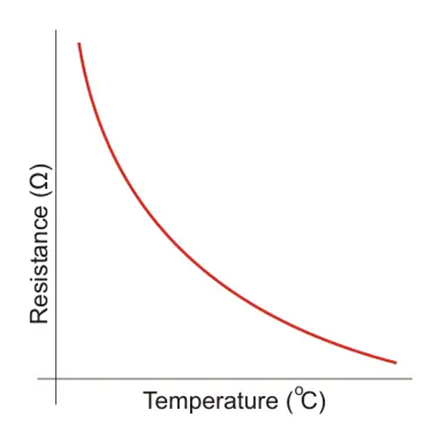
\includegraphics[width=4.7cm,height=5cm]{Images/pttemp.png}
		\caption[Biều đồ sự ảnh hưởng của nhiệt độ tới trở nhiệt\cite{NTC}]{\bfseries \fontsize{12pt}{0pt}\selectfont Biều đồ sự ảnh hưởng của nhiệt độ tới trở nhiệt\cite{NTC}}
		\label{pttemp}
	\end{figure}
	
	
	Cảm biến nhiệt độ NTC(Negative Temperature Coefficient) là một loại của trở nhiệt, cách hoạt động của cảm biến tương đương với cách hoạt động của trở nhiệt. Cảm biến nhiệt độ hoạt động trên nguyên lý khi nhiệt độ tăng thì điện trở giảm và khi nhiệt độ giảm, điện trở tăng. Do đó, nhiệt độ và điện trở nhiệt điện trở NTC tỷ lệ nghịch với nhau. Mối quan hệ giữa điện trở và nhiệt độ trong một nhiệt điện trở NTC được điều chỉnh bởi biểu thức sau\cite{NTC}: 
	
	\begin{equation}
		R_T = R_0 \cdot e^{\beta \left(\frac{1}{T} - \frac{1}{T_0}\right)}
	\end{equation}
	
	
	Trong đó :
	
	\begin{itemize}
		\item $R_T$ :Giá trị điện trở tại nhiệt độ T(Kelvin)
		\item $R_0$ :Giá trị điẹn trở tại nhiệt độ $T_0$(K)
		\item $T_0$ :Giá trị nhiệt độ tham chiếu (25\textdegree C)
		\item T :Giá trị nhiệt độ hiện tại(K)
		\item beta : là một hằng số. mốt giá trị của nó phụ thuộc vào đặc tính của vật liệu thông thường khoảng 4000.
	\end{itemize}
	
	Cảm biến NTC 10K$\Omega$ Hình \ref{NTC10k} là cảm biến trở nhiệt có tính kháng nước cao và nhạy cảm với sự thay đổi của nhiệt.Vậy nên trong đề tài này em sử dụng cảm biến NTC10K để đo giá trị nhiệt độ môi trường nước.
	
	\begin{figure}[!ht]
		\centering
		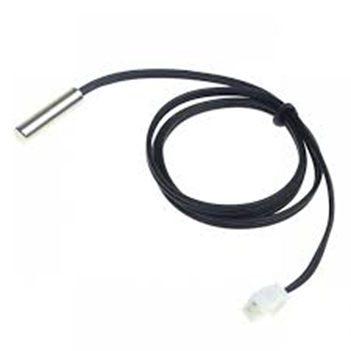
\includegraphics[width=4cm,height=5cm]{Images/NTC10k.png}
		\caption[Cảm biến nhiệt độ NTC 10k$\Omega$ \cite{NTC}]{\bfseries \fontsize{12pt}{0pt}\selectfont Cảm biến nhiệt độ NTC10k$\Omega$ \cite{NTC}}
		\label{NTC10k}
	\end{figure}
	
	Thông số của cảm biến NTC 10k$\Omega$:
	\begin{itemize}
		\item Vùng nhiệt độ làm việc : -40\textdegree C đến 125\textdegree C
		\item Giá trị điện trở ở nhiệt độ $T_0$=25\textdegree C : 10k$\Omega$
		\item Hệ số Beta :3478
	\end{itemize}
	
	\subsubsection{Lý thuyết về module chuyển đổi tương tự ADC}
	
	ADC (Analog to Digital Converter) hay bộ chuyển đổi analog sang kỹ thuật số là một mạch chuyển đổi giá trị điện áp liên tục (analog) sang giá trị nhị phân (kỹ thuật số) mà thiết bị có thể hiểu được sau đó có thể được sử dụng để tính toán kỹ thuật số.
	
	\begin{figure}[!ht]
		\centering
		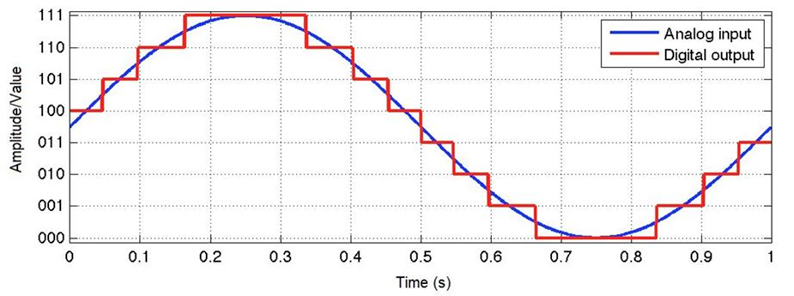
\includegraphics[width=9.5cm,height=4.2cm]{Images/ADC.png}
		\caption[Ví dụ về cách hoạt động của bộ chuyển đổi ADC\cite{Analog}]{\bfseries \fontsize{12pt}{0pt}\selectfont Ví dụ về cách hoạt động của bộ chuyển đổi ADC\cite{Analog}}
		\label{ADC}
	\end{figure}
	
	Trong Hình \ref{ADC}, đường màu xanh thể hiện cho tín hiệu tương tực, đường màu đỏ thể hiện cho tín hiệu tái tạo từ bộ ADC. Trục tung thể hiện cho các mức điện áp, các mức điện áp được quyết định với số bit trong bộ ADC, trục hoành thể hiện cho thời gian. Bộ ADC có chức năng so sánh điện áp của mỗi lần lấy mẫu với các mức điện áp, kết quả của bộ đo là chuỗi số nhị phân tương ứng với mức điện áp lớn gần bằng điện áp mẫu hay mức điện áp lớn nhất mà điện áp lẫy mẫu lớn hơn tùy thuộc vào cách hoạt động của từng bộ ADC.
	
	ADC thực hiện chức năng chuyển đổi tín hiệu tương tự sang tín hiệu số. Sau quá trình chuyển đổi, kết quả thu được là một chuỗi bit có độ dài tùy thuộc vào độ phân giải của bộ ADC. Độ phân giải của bộ ADC càng cao sẽ làm cho tỷ lệ chính xác càng cao. Đối với bất kỳ bộ ADC nào, công thức liên hệ với độ phân giải sẽ như sau: 
	
	\begin{equation}
		\Delta = \frac{v_{\text{ref}}}{N}    
	\end{equation}
	
	Trong đó:
	\begin{itemize}
		\item \( \Delta \) là độ phân giải của mỗi cấp độ điện áp
		\item \( v_{\text{ref}} \) là điện áp tham chiếu
		\item \( N \) là kích thước của bộ ADC hay số mức của bộ ADC
	\end{itemize}
	
	Để tìm được N , ta có công thức :
	\begin{equation}
		N = {2}^{n}
	\end{equation}
	Trong đó:
	\begin{itemize}
		\item \( n \) là số bit của bộ ADC
	\end{itemize}
	
	Để hiểu rõ hơn về độ phân giải của bộ ADC thông qua Hình \ref{ADCconvert} sau:
	
	\begin{figure}[!ht]
		\centering
		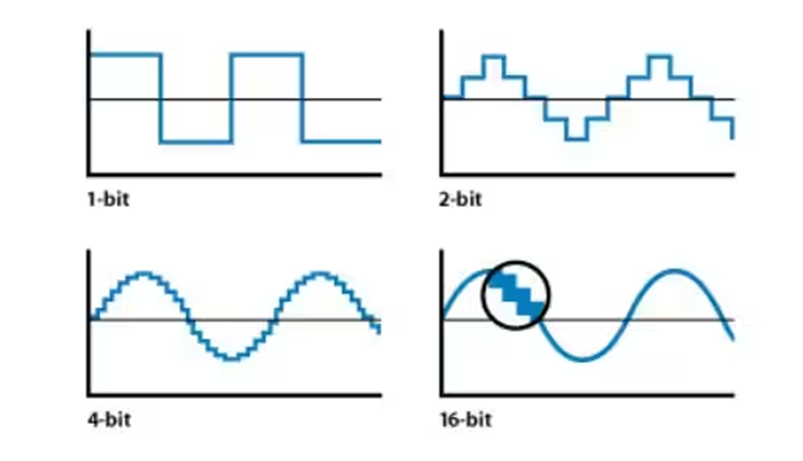
\includegraphics[width=8cm,height=4cm]{Images/ADCconvert.png}
		\caption[Hình so sánh sự ảnh hưởng của độ phân giải tới bộ chuyển đổi ADC\cite{Analog}]{\bfseries \fontsize{12pt}{0pt}\selectfont Hình so sánh sự ảnh hưởng của độ phân giải tới bộ chuyển đổi ADC\cite{Analog}}.
		\label{ADCconvert}
	\end{figure}
	
	Từ Hình \ref{ADCconvert}, ta có thể thấy với độ phân giải càng cao, sự chênh lệch của mỗi mức điện áp càng nhỏ và độ chính xác càng cao.
	
	\newpage
	\subsection{Tổng quan về Internet of Things}
	\subsubsection{Giới thiệu}
	
	Thuật ngữ IoT hay Internet vạn vật đề cập đến mạng lưới tập hợp các thiết bị thông minh và công nghệ tạo điều kiện thuận lợi cho hoạt động giao tiếp giữa thiết bị và đám mây cũng như giữa các thiết bị với nhau. Nhờ sự ra đời của chip máy tính giá rẻ và công nghệ viễn thông băng thông cao, ngày nay, chúng ta có hàng tỷ thiết bị được kết nối với internet. Điều này nghĩa là các thiết bị hàng ngày như bàn chải đánh răng, máy hút bụi, ô tô và máy móc có thể sử dụng cảm biến để thu thập dữ liệu và phản hồi lại người dùng một cách thông minh.
	
	\begin{figure}[!ht]
		\centering
		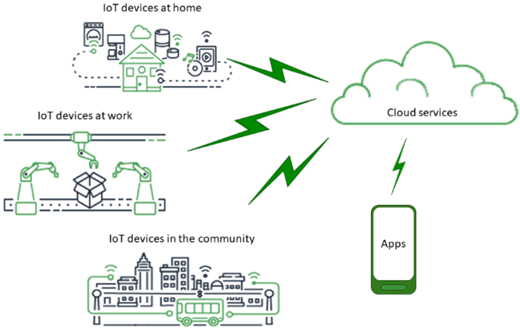
\includegraphics[width=7cm,height=4cm]{Images/introIOT.png}
		\caption[Mô hình hệ thống IOT\cite{IOT}]{\bfseries \fontsize{12pt}{0pt}\selectfont Mô hình hệ thống IOT\cite{IOT}}
		\label{introIOT}
	\end{figure}
	
	Một hệ thống IoT thông thường hoạt động thông qua việc thu thập và trao đổi dữ liệu theo thời gian thực. Theo Hình \ref{introIOT}, một hệ thống IoT có ba thành phần:
	
	
	\begin{itemize}
		\item Thiết bị thông minh
		
		Đây là một thiết bị, giống như tivi, camera an ninh hoặc thiết bị tập thể dục đã được trao cho khả năng điện toán. Thiết bị này thu thập dữ liệu từ môi trường xung quanh, thao tác nhập liệu của người dùng hoặc mô thức sử dụng và truyền cũng như nhận dữ liệu qua Internet từ ứng dụng IoT của nó.
		
		\item Ứng dụng IOT % You can add more items here following the same format
		
		Ứng dụng IoT là một tập hợp các dịch vụ và phần mềm có chức năng tích hợp dữ liệu nhận được từ các thiết bị IoT khác nhau. Ứng dụng này sử dụng công nghệ máy học hoặc trí tuệ nhân tạo (AI) để phân tích dữ liệu và đưa ra các quyết định sáng suốt. Những quyết định này được truyền trở lại thiết bị IoT và sau đó, thiết bị IoT đó sẽ phản hồi lại dữ liệu đầu vào một cách thông minh. 
		\item Giao diện đồ họa người dùng
		
		Một hoặc một nhóm các thiết bị IoT có thể được quản lý thông qua giao diện đồ họa người dùng. Các ví dụ phổ biến bao gồm một ứng dụng di động hoặc trang web có thể được sử dụng để đăng ký và kiểm soát các thiết bị thông minh.
	\end{itemize}
	
	
	\subsubsection{ Cấu trúc của một IOT}
	
	\begin{figure}[!ht]
		\centering
		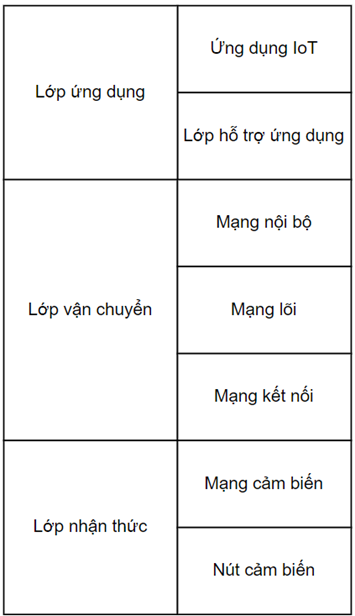
\includegraphics[width=4cm,height=7cm]{Images/iotstructure.png}
		\caption[Kiến trúc của một IOT\cite{jing2014security}]{\bfseries \fontsize{12pt}{0pt}\selectfont Kiến trúc của một IOT\cite{jing2014security}}
		\label{iotstructure}
	\end{figure}
	
	IoT không có kiến trúc chuẩn, Hình \ref{iotstructure} dựa theo kiến trúc đề xuất của ITU-T Y.2002, IoT được chia làm 3 lớp: lớp nhận thức, lớp vận chuyển, lớp ứng dụng.
	
	\begin{itemize}
		\item Lớp nhận thức: chức năng chính yếu của lớp này là thu thập thông tin, lớp này có thể chia ra làm 2 phần: nút nhận thức (cảm biến, vi điều khiển, …) và phần mạng nhận thức để giao tiếp với lớp vận chuyển phía trên. Nút nhận thức sẽ đảm nhiệm kiểm soát và thu thập dữ liệu, phần mạng nhận thức sẽ gửi dữ liệu thu thập được lên gateway hoặc gửi tín hiệu điều khiển về vi điều khiển.
		\item Lớp vận chuyển (Transportation): nhiệm vụ chủ yếu là cung cấp môi trường truy cập cho tầng Perception, truyền thông tin và lưu trữ thông tin, và tải các hoạt động liên quan khác của tầng ứng dụng. Tầng Transportation có thể chia thành ba tầng con theo chức năng: mạng truy cập, mạng trung tâm và mạng khu vực. Đây là sự kết hợp của nhiều mạng không đồng nhất.
		\item Lớp ứng dụng: là một tầng nằm phía trên tầng Transportation, hỗ trợ các dịch vụ kinh doanh đa dạng và thực hiện tính toán thông minh và phân bổ tài nguyên trong quá trình lọc, chọn lọc, sản xuất và xử lý dữ liệu. Trong suốt quá trình đó, tầng hỗ trợ ứng dụng có thể nhận ra dữ liệu hợp lệ, dữ liệu spam và thậm chí dữ liệu độc hại, và lọc chúng kịp thời. Tầng hỗ trợ ứng dụng có thể được tổ chức theo các cách khác nhau tùy theo các dịch vụ khác nhau. Thông thường, nó bao gồm phần mềm trung gian, M2M, nền tảng cloud computing và nền tảng hỗ trợ dịch vụ.
		
	\end{itemize}
	
	
	\subsubsection{Ứng dụng của IOTsub}
	
	Có rất nhiều ứng dụng của IoT đối với thực tiễn, một số các ứng dụng hàng đầu của IoT như hình Hình \ref{UngdungIOT}.
	
	\begin{figure}[!ht]
		\centering
		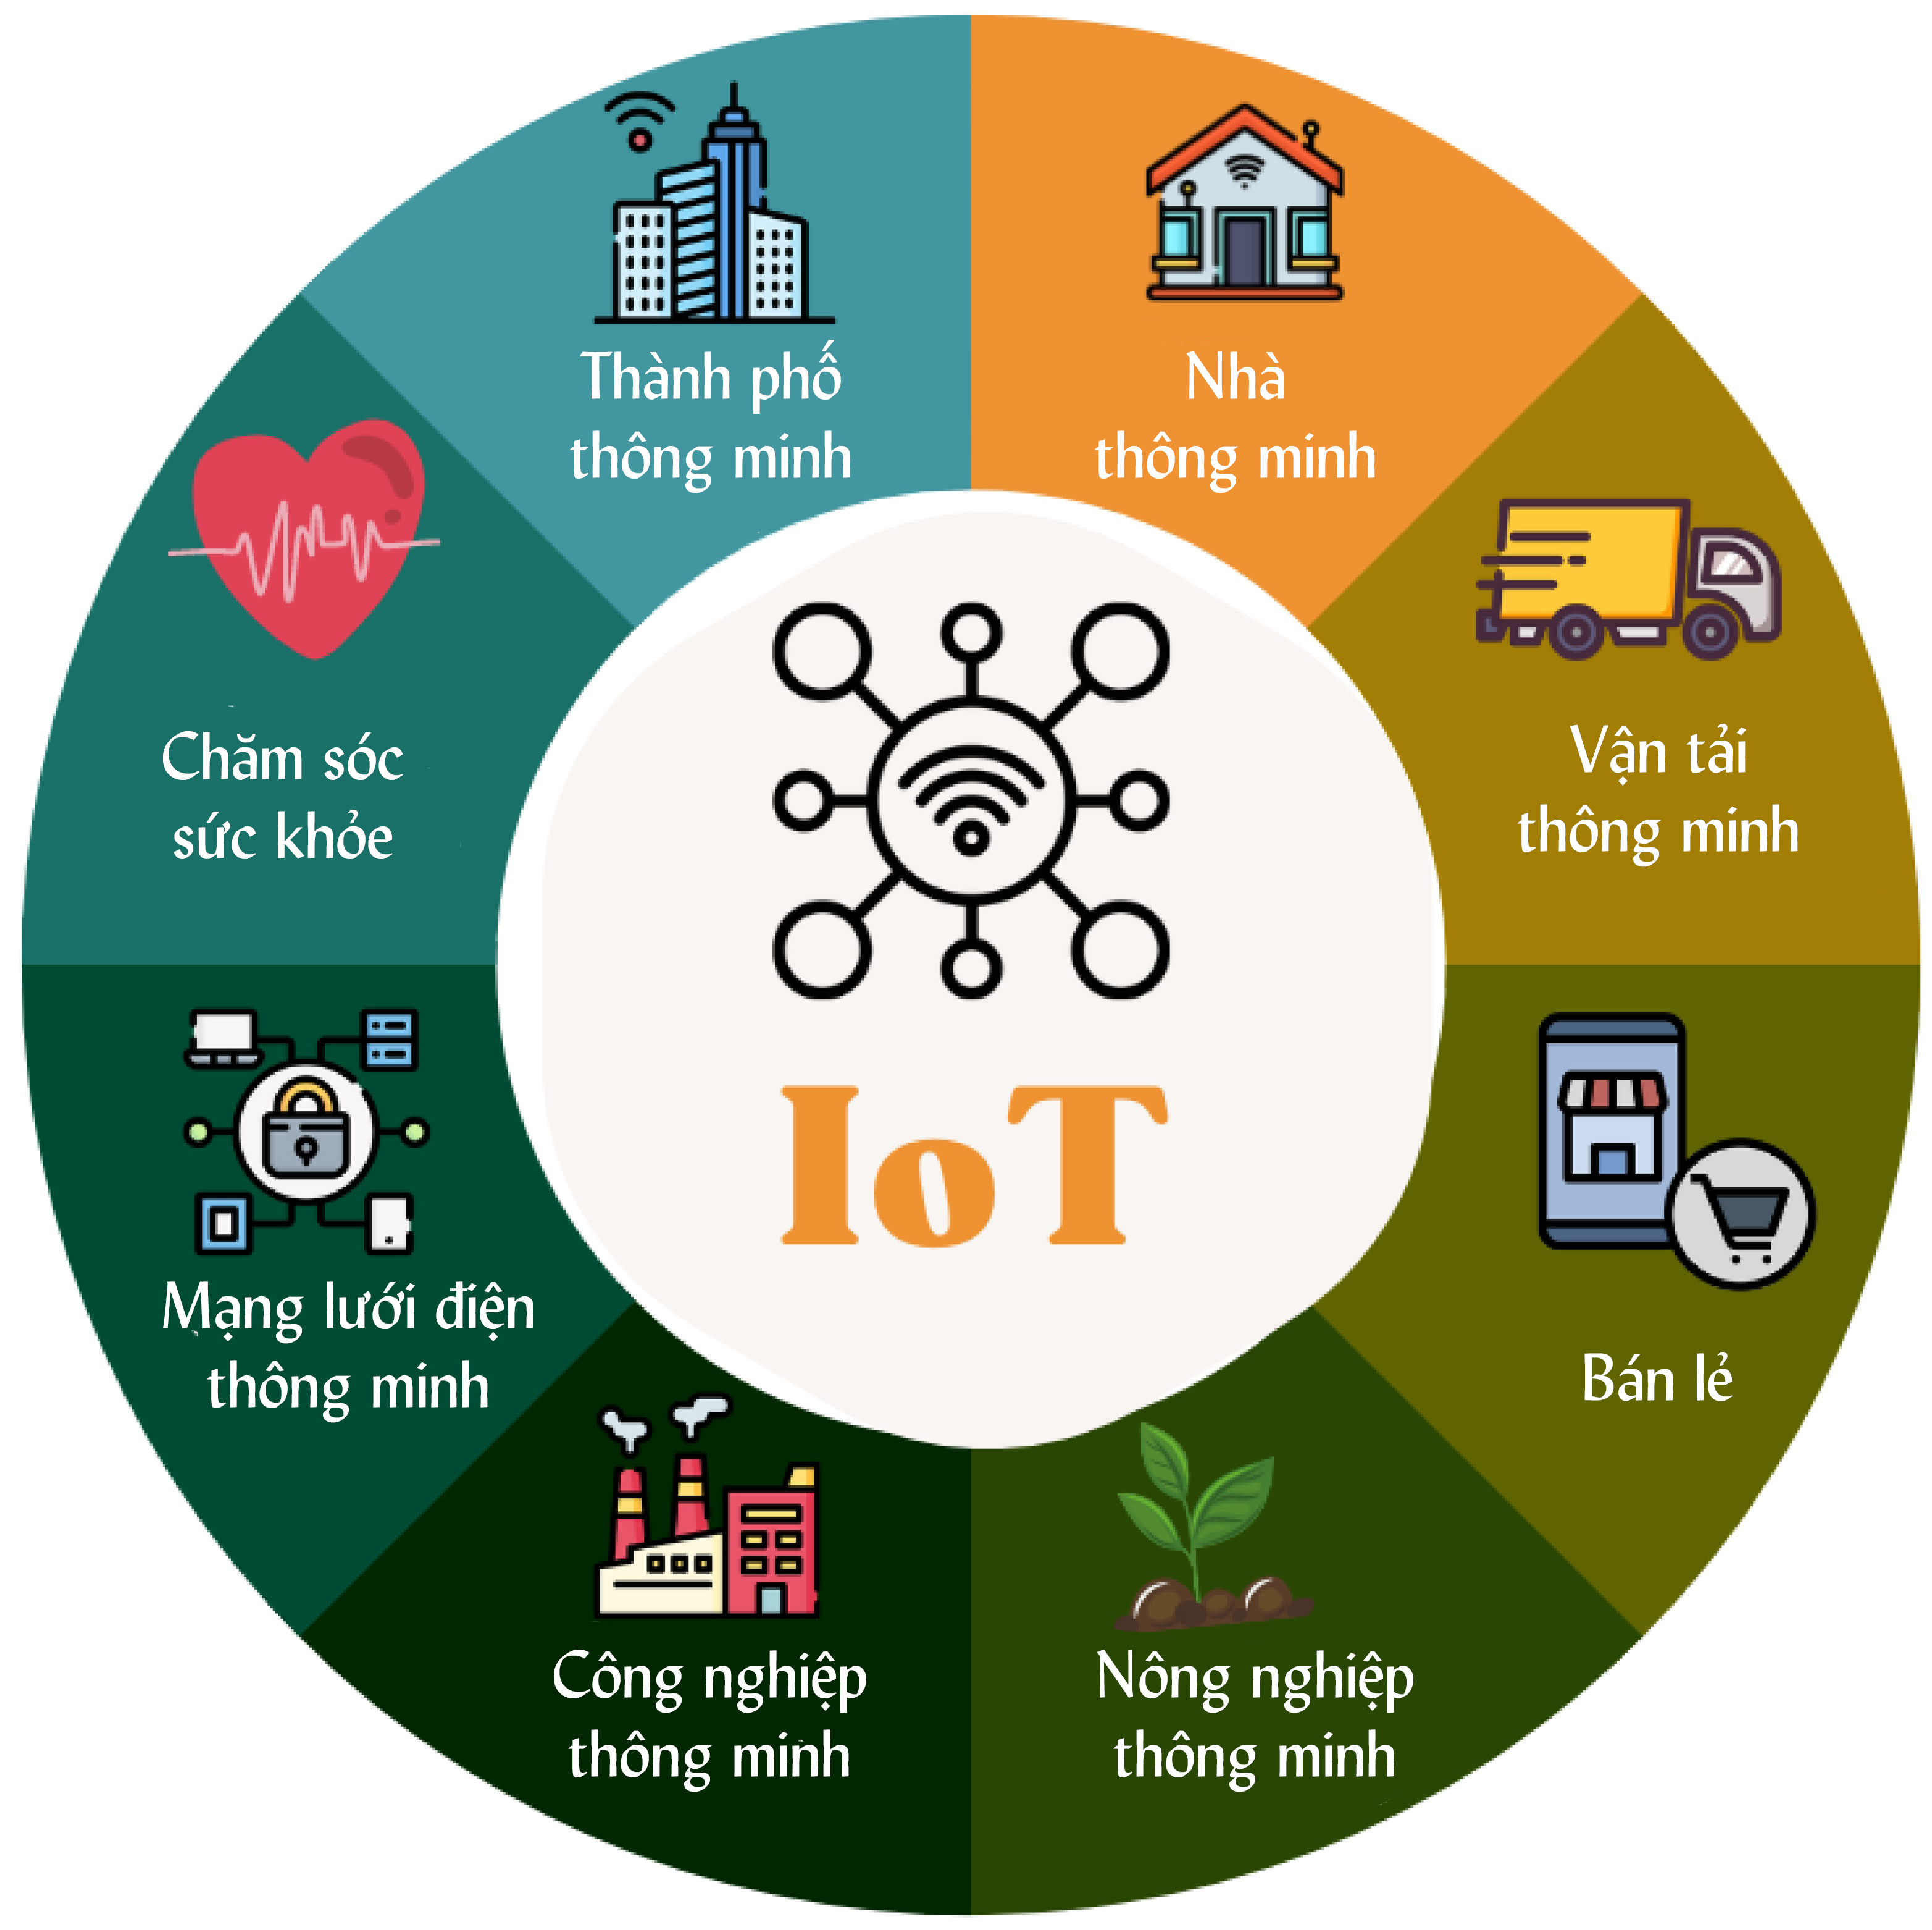
\includegraphics[width=6cm,height=6cm]{Images/UngdungIOT.jpg}
		\caption[Ứng dụng của IOT \cite{uNGDUNGiot}]{\bfseries \fontsize{12pt}{0pt}\selectfont Ứng dụng của IOT\cite{uNGDUNGiot}}
		\label{UngdungIOT}
	\end{figure}
	
	\begin{itemize}
		\item Được Giám sát sức khỏe từ xa: Lợi ích chính của hệ thống giám sát sức khỏe từ xa là giúp bệnh nhân có thể sống cuộc sống bình thường dù đang được giám sát sức khỏe liên tục. Sử dụng các hệ thống cảm biến tự động gắn trên quần áo của bệnh nhân để thu thập các thông số sức khỏe và dữ liệu đã thu thập được xử lý. Sau đó, dữ liệu đã được xử lý được truyền đến máy chủ trung tâm để lưu trữ và phân tích giúp bác sĩ có thể theo dõi sức khỏe của bệnh nhân từ xa.
		\item Nhà thông minh: Internet of Things đã định nghĩa lại cách điều khiển các thiết bị điện tử trong môi trường nhà ở. Mọi thiết bị như đèn, máy điều hòa không khí, hệ thống truyền thông, hệ thống an ninh, tủ lạnh, lò nướng và các thiết bị khác có thể kết nối với internet bằng cách sử dụng công tắc relay, vi điều khiển và thiết bị mạng. Bằng cách sử dụng giao diện đồ họa, người dùng có thể điều khiển các thiết bị ngay cả từ xa. Có rất nhiều loại cảm biến được phát triển để triển khai hệ thống tự động hóa nhà thông minh dựa trên IoT.
		\item Thương mại thông minh: Một trong những đặc điểm của IoT là cung cấp một danh tính duy nhất cho các đối tượng người dùng. Đặc điểm này được sử dụng trong việc phát triển hệ thống theo dõi tài sản người tiêu dùng. Hiện nay, hầu hết các điện thoại di động được trang bị hệ thống theo dõi GPS cho phép dễ dàng xác định vị trí của điện thoại bị mất. Tương tự cơ chế đó, IoT cho phép áp dụng tính năng này cho các tài sản người tiêu dùng bằng cách cung cấp một danh tính duy nhất và kết nối internet cho các tài sản đó. Các công ty thương mại điện tử có thể theo dõi tình trạng sản phẩm trong quá trình vận chuyển để đảm bảo việc giao hàng đúng. Các cảm biến gia tốc, GPS, cảm biến rung động, RFID là một phần của hệ thống. Các bộ xử lý mạng nano được sử dụng để thiết lập kết nối internet với các dịch vụ đám mây
		\item Giao tiếp giữa các phương tiện giao thông: Internet of Things mở ra một chiều sâu mới trong việc giao tiếp xe cộ, bao gồm giao tiếp giữa xe và cảm biến, giữa các xe và giao tiếp giữa xe và internet. Giao tiếp xe cộ có thể được phân loại thành hai loại: giao tiếp trong xe và giao tiếp giữa các xe. Hệ thống giao tiếp trong xe bao gồm một mạng cảm biến để giám sát điều kiện đường, sự mệt mỏi của tài xế, áp suất lốp và nhiệt độ nước trong hệ thống làm mát và những điều tương tự. Giao tiếp xe cộ là kết nối giữa các xe để tránh tai nạn, truyền thông tin về việc thay đổi làn đường, v.v.v. IoT có thể cung cấp việc nâng cấp dễ dàng cho các xe thành các xe thông minh bằng cách thiết kế kiến trúc phù hợp và lựa chọn các giao thức truyền thông nhẹ để thiết lập giao tiếp giữa các xe.
		\item Kiểm soát năng lượng thông minh: Có thể nâng cấp công nghệ trên mạng lưới điện truyền thống bằng cách tích hợp IoT để chuyển đổi nó thành một mạng lưới thông minh. Mạng lưới thông minh có thể được xác định là một hệ thống IoT có khả năng cảm nhận từ các thành phần khác nhau của lưới và thiết lập một hệ thống quản lý nguồn điện dựa trên việc điều khiển cung cấp điện theo nhu cầu. Điều này cung cấp sự tương tác chính xác và nhanh chóng giữa khách hàng và các công ty điện lưới. Nhờ giám sát trực tuyến liên tục, việc khôi phục tự động có thể được thực hiện khi xảy ra sự cố bằng cách thực hiện kiểm soát trước.
	\end{itemize}
	
	\subsection{Một số giao thức truyền tải dữ liệu trong IoT}
	\subsubsection{ Giao thức truyền thông MQTT}
	
	MQTT (Message Queue Telemetry Transport) là một giao thức mã nguồn mở để truyền các messages giữa nhiều Client (Publisher và Subscriber) thông qua một Broker trung gian, được thiết kế để đơn giản và dễ dàng triễn khai. Kiến trúc MQTT dựa trên Broker trung gian và sử dụng kết nối TCP long-lived từ các Client đến Broker. Hình \ref{MQTT} cho ta thấy tổng quát mô hình hạ tầng giao tiếp MQTT.
	
	\begin{figure}[!ht]
		\centering
		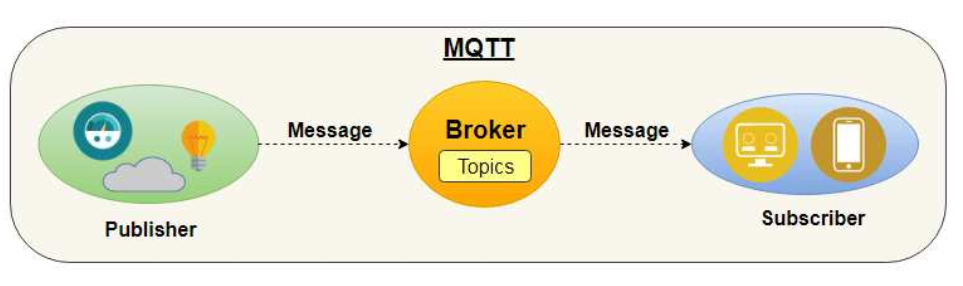
\includegraphics[width=9cm,height=4cm]{Images/MQTT.png}
		\caption[Mô hình sử dụng giao thức MQTT\cite{ansari2018internet}]{\bfseries \fontsize{12pt}{0pt}\selectfont Mô hình sử dụng giao thức MQTT\cite{ansari2018internet}}
		\label{MQTT}
	\end{figure}
	\newpage
	Là giao thức hỗ trợ tổ chức hệ thống theo các Topics có tính phân cấp, như một hệ thống tập tin, cung cấp nhiều lựa chọn điều khiển và QoS (Quality of Service). Có thể được sử dụng cho truyền thông 2 chiều thông qua các mạng có độ trễ cao và độ tin cậy thấp, nó cũng tương thích với các thiết bị tiêu thụ điện năng thấp.
	
	\subsubsection{Giao thức truyền thông CoAP}
	
	CoAP (Constrained Applications Protocol) là một giao thức truyền tải tài liệu theo mô hình client/server dự trên internet tương tự như giao thức HTTP nhưng được thiết kế cho các thiết bị ràng buộc. Giao thức này hỗ trợ một giao thức one-to-one để chuyển đổi trạng thái thông tin giữa client và server.
	
	
	Hình \ref{HTTP} là mô hình của một hệ thống kết hợp CoAP cho môi trường có ràng buộc và HTTP, CoAP sử dụng UDP (User Datagram Protocol), không hỗ trợ TCP, ngoài ra còn hỗ trợ địa chỉ broadcast và multicast, truyền thông CoAP thông qua các datagram phi kết nối (connectionless) có thể được sử dụng trên các giao thức truyền thông dựa trên các gói. Cho nên có thể dễ dàng triển khai trên các vi điều khiển hơn TCP nhưng các công cụ bảo mật như SSL/TSL không có sẵn, tuy nhiên ta có thể sử dụng Datagram Transport Layer Security (DTLS) để thay thế.
	
	\begin{figure}[!ht]
		\centering
		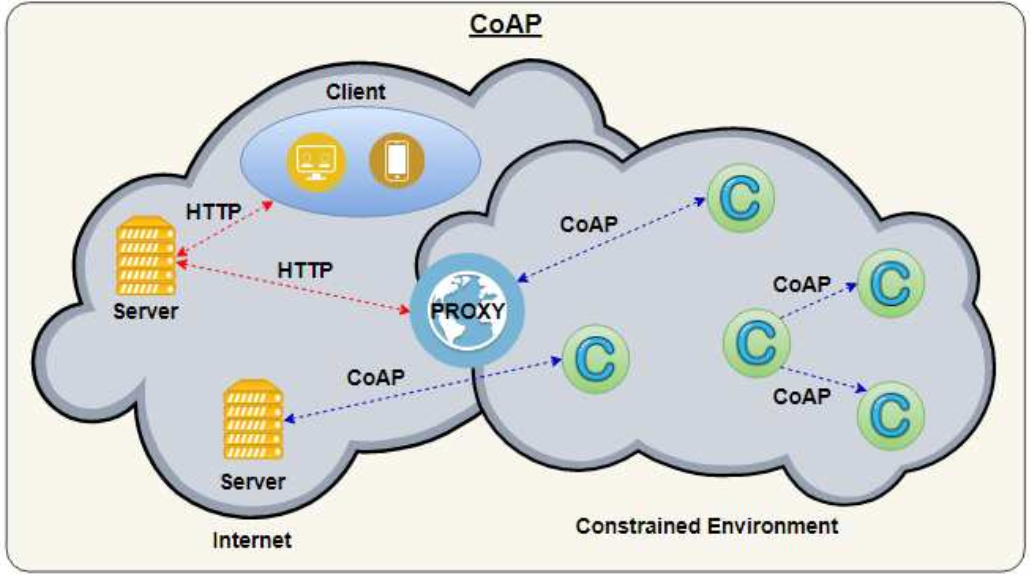
\includegraphics[width=9cm,height=5cm]{Images/HTTP.png}
		\caption[Mô hình sử dụng giao thức CoAP và HTTP\cite{ansari2018internet}]{\bfseries \fontsize{12pt}{0pt}\selectfont Mô hình sử dụng giao thức CoAP và HTTP\cite{ansari2018internet}}
		\label{HTTP}
	\end{figure}
	
	
	\subsection{Mạng LPWAN ứng dụng cho IOT}
	\subsubsection{Giới thiệu về Mạng LPWAN}
	
	Mạng LPWAN (Hình \ref{LPWANAPP})là một loại mạng viễn thông được thiết kế để cho phép truyền thông tin không dây với công suất thấp, khoảng cách xa, và tốc độ truyền dữ liệu tương đối thấp. LPWAN đặc biệt phù hợp cho các ứng dụng IoT (Internet of Things) và M2M (Machine to Machine), nơi yêu cầu các thiết bị tiêu thụ ít năng lượng và có khả năng truyền dữ liệu qua khoảng cách rộng lớn.
	
	\begin{figure}[!ht]
		\centering
		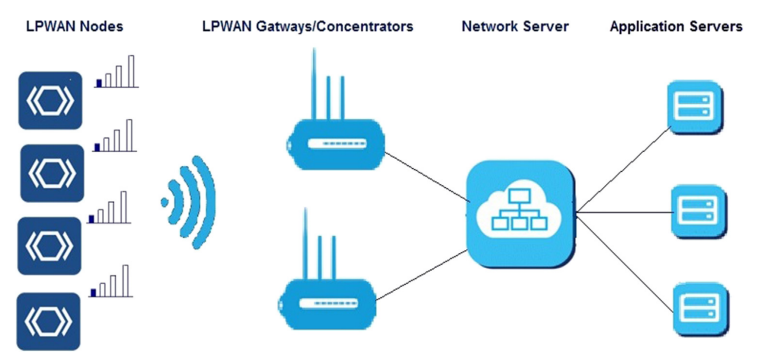
\includegraphics[width=9cm,height=5cm]{Images/LPWANAPP.png}
		\caption[Mô hình mạng LPWAN \cite{chaudhari2020lpwan}]{\bfseries \fontsize{12pt}{0pt}\selectfont Mô hình mạng LPWAN \cite{chaudhari2020lpwan}}
		\label{LPWANAPP}
	\end{figure}
	\subsubsection{Đặc điểm của LPWAN}
	
	\begin{itemize}
		\item Công suất thấp: LPWAN được tối ưu hóa để tiêu thụ năng lượng thấp, cho phép các thiết bị hoạt động bằng pin trong nhiều năm mà không cần thay thế.
		\item Phạm vi rộng: LPWAN có khả năng truyền dữ liệu qua khoảng cách xa, thường từ vài km đến hàng chục km, phù hợp cho việc giám sát và quản lý các thiết bị phân tán.
		\item Tốc độ truyền dữ liệu thấp: LPWAN hỗ trợ tốc độ truyền dữ liệu thấp, thường từ vài kbps đến vài trăm kbps, đủ để truyền các gói dữ liệu nhỏ và không yêu cầu băng thông cao.
		\item Chi phí thấp: LPWAN thường có chi phí triển khai và vận hành thấp, làm cho nó trở thành giải pháp kinh tế cho các ứng dụng IoT.
	\end{itemize}
	
	\subsubsection{Các công nghệ LPWAN phổ biến}
	
	\begin{itemize}
		\item LoRa (Long Range): LoRa là công nghệ LPWAN không được cấp phép hoạt động ở tần số dưới gigahertz. Nó sử dụng điều chế trải phổ chirp (CSS), mang lại khả năng chống nhiễu mạnh mẽ và cho phép liên lạc tầm xa. LoRa cung cấp tính linh hoạt về tốc độ dữ liệu và sơ đồ điều chế để đáp ứng các yêu cầu ứng dụng khác nhau. Chip thu phát độc quyền của Semtech Corporation rất cần thiết cho việc triển khai LoRa. Giao thức LoRaWAN quản lý hoạt động liên lạc giữa các thiết bị và cổng LPWAN, khiến nó trở thành lựa chọn phổ biến để triển khai IoT tiết kiệm pin, chi phí thấp.
		\begin{itemize}
			\item Phạm vi: lên đến 15 km ở môi trường nông thôn và vài km ở môi trường đô thị.
			\item Tần số hoạt động: 433 MHz, 868 MHz (Châu Âu), 915 MHz (Bắc Mỹ).
		\end{itemize}
		
		\item Sigfox: Sigfox là một công nghệ LPWAN không được cấp phép khác hoạt động ở phổ tần dưới gigahertz. Nó sử dụng một giao thức độc quyền duy nhất để cho phép liên lạc tầm xa, tiêu thụ điện năng thấp. Sigfox cung cấp một giải pháp đơn giản và tiết kiệm chi phí để kết nối nhiều thiết bị trên một khu vực rộng, nhưng nó có khả năng hạn chế về băng thông và tốc độ dữ liệu. Các thiết bị Sigfox có phạm vi hoạt động tối đa 40 km ở môi trường ngoài trời và 10 km ở khu vực thành thị.
		\begin{itemize}
			\item Phạm vi: lên đến 50 km ở môi trường nông thôn và 10 km ở môi trường đô thị.
			\item Tần số hoạt động: 868 MHz (Châu Âu), 915 MHz (Bắc Mỹ).
		\end{itemize}
		
		\item NB-IoT (Narrowband IoT): NB-IoT là công nghệ LPWAN dựa trên thiết bị di động được chuẩn hóa bởi Dự án Đối tác Thế hệ thứ 3 (3GPP). Nó hoạt động trên phổ tần được cấp phép, tận dụng cơ sở hạ tầng di động hiện có. NB-IoT cung cấp khả năng phủ sóng và thâm nhập tuyệt vời, rất phù hợp cho các ứng dụng yêu cầu phủ sóng sâu trong nhà hoặc triển khai ở các vùng sâu vùng xa. Nó sử dụng công nghệ băng thông hẹp để cho phép sử dụng hiệu quả tài nguyên phổ tần và kết nối đồng thời cho một số lượng lớn thiết bị.
		\begin{itemize}
			\item Phạm vi: lên đến 35 km.
			\item Tần số hoạt động: sử dụng băng tần LTE hiện có.
		\end{itemize}    
	\end{itemize}
	
	
	\subsubsection{Ứng dụng của công nghệ LPWAN}
	\begin{itemize}
		\item Thành phố thông minh : LPWAN cho phép các giải pháp thành phố thông minh như chiếu sáng thông minh, quản lý chất thải, quản lý bãi đậu xe và giám sát môi trường. Các ứng dụng này góp phần cải thiện hiệu quả đô thị, tính bền vững và phúc lợi chung của cư dân.
		
		\item IoT công nghiệp : LPWAN hỗ trợ giám sát từ xa, bảo trì dự đoán và theo dõi tài sản trong môi trường công nghiệp. Bằng cách khai thác LPWAN, doanh nghiệp có thể tối ưu hóa hoạt động, nâng cao năng suất và giảm thời gian ngừng hoạt động.
		
		\item Nông nghiệp và Trồng trọt : Bằng cách tận dụng LPWAN, nông nghiệp chính xác được cải thiện khi dữ liệu thời gian thực về độ ẩm đất, nhiệt độ và sức khỏe cây trồng được cung cấp. Thông tin này cho phép nông dân đưa ra quyết định sáng suốt, cải thiện việc sử dụng tài nguyên và cuối cùng là tăng năng suất.
		
		\item Theo dõi tài sản và hậu cần : Công nghệ LPWAN giúp theo dõi và giám sát tài sản trong chuỗi cung ứng, đảm bảo hoạt động hậu cần hiệu quả và giảm tổn thất.
		
		\item Giám sát môi trường : LPWAN hỗ trợ quản lý môi trường tốt hơn, cho phép giám sát các thông số môi trường bao gồm chất lượng không khí, chất lượng nước và mức độ tiếng ồn.
		\item Chăm sóc sức khỏe thông minh : Tăng cường cung cấp dịch vụ chăm sóc sức khỏe và chăm sóc bệnh nhân, công nghệ LPWAN cho phép theo dõi bệnh nhân từ xa, theo dõi tài sản trong bệnh viện và theo dõi nhiệt độ thuốc.
		
	\end{itemize}
	
	
	
	\subsection{Công nghệ truyền thông Lora}
	\subsubsection{Giới thiệu}
	
	LoRa, viết tắt của "Long Range", là một công nghệ truyền thông không dây được phát triển nhằm phục vụ các ứng dụng cần truyền dữ liệu qua khoảng cách lớn và sử dụng ít năng lượng. Công nghệ này sử dụng kỹ thuật trải phổ và điều chế chirp để truyền dữ liệu qua các tần số từ 137 MHz đến 1020 MHz, nhưng thường hoạt động trong một số tần số thuộc dải ISM như: 169 MHz, 433 MHz, 868 MHz và 915 MHz. LoRa rất phù hợp cho các ứng dụng mạng cảm biến không dây do khả năng truyền một lượng nhỏ dữ liệu. Đáng chú ý, LoRa là ứng dụng thương mại đầu tiên của kỹ thuật trải phổ chirp.
	
	Khả năng truyền thông xa và tiêu thụ năng lượng thấp của LoRa được nhờ vào kỹ thuật điều chế trải phổ chirp. Mặc dù Semtech giữ bí mật về Modulation Scheme này, nhưng nó chắc chắn được phát triển dựa trên kỹ thuật Chirp Spread-spectrum modulation. LoRa sử dụng các hệ số trải phổ trực giao để cung cấp các tốc độ dữ liệu (data rate) và mức tiêu thụ năng lượng khác nhau cho các ứng dụng cụ thể. Sự kết hợp giữa ba tham số chính: băng thông (bandwidth), tỷ lệ mã hóa (coding rate) và hệ số trải phổ (spreading factor), tạo ra các chế độ truyền thông khác nhau của LoRa. Semtech đã cung cấp một công thức tính toán thời gian hoạt động trên không (Time on the Air - ToA), là hàm số kết hợp của SF (Spreading Factor), CR (Coding Rate), BW (Bandwidth) và kích thước payload. Để hiểu rõ hơn về kỹ thuật điều chế LoRa, cần nắm bắt một số khái niệm kỹ thuật cơ bản, sẽ được trình bày chi tiết trong các phần tiếp theo.
	
	
	\subsubsection{Công thức Shannon – Hartley}
	Trong lý thuyết thông tin, định lý Shannon-Hartle [2] chỉ ra tốc độ tối đa truyền tin ở một kênh truyền thông. Với một kênh truyền có tham số băng thông và bị ảnh hưởng bởi nhiễu, dung lượng của một kênh truyền được tính như sau \cite{semtech2015an1200}:
	
	\begin{equation}\label{Shannon_Hartley}
		C=B \times \log _2\left(1+\frac{S}{N}\right)
	\end{equation}
	
	Trong đó:
	\begin{itemize}
		\item C là dung lượng kênh tính bằng bit trên giây.
		\item B là băng thông kênh (Hertz).
		\item S là tổng công suất của tín hiệu nhận trên băng thông B.
		\item N là tổng công suất nhiễu trên kênh.
		\item S/N là tỷ số SNR của kênh.
	\end{itemize}
	
	Sau khi tính $log _2$  ta có biểu thức $\frac{C}{B}=1.433 \times \frac{S}{N}$ ,công thức trên cho thấy rằng, nếu muốn tăng dung lượng kênh thì có thể cố định tỷ số SNR mà tăng băng thông kênh truyền. Điều này là ý tưởng cơ bản của kỹ thuật điều chế trải phổ.
	
	
	\subsubsection{Kĩ thuật trải phổ }	
	
	Theo công thức của Shannon, khi băng thông tín hiệu được tăng lên, tác động của nhiễu có thể giảm thiểu đáng kể. Kỹ thuật trải tín hiệu trên miền tần số được gọi là kỹ thuật trải phổ. Có nhiều loại kỹ thuật trải phổ, trong đó một trong những kỹ thuật cơ bản nhất là kỹ thuật trải phổ trực tiếp (DSSS). DSSS sử dụng một mã có tần số cao hơn tín hiệu dữ liệu để trải phổ tần số của tín hiệu cần truyền Hình \ref{Traipho}. Mã này, gọi là mã trải phổ hoặc chuỗi chip (chip sequence), được nhân với tín hiệu dữ liệu trước khi truyền đi.
	
	\begin{figure}[!ht]
		\centering
		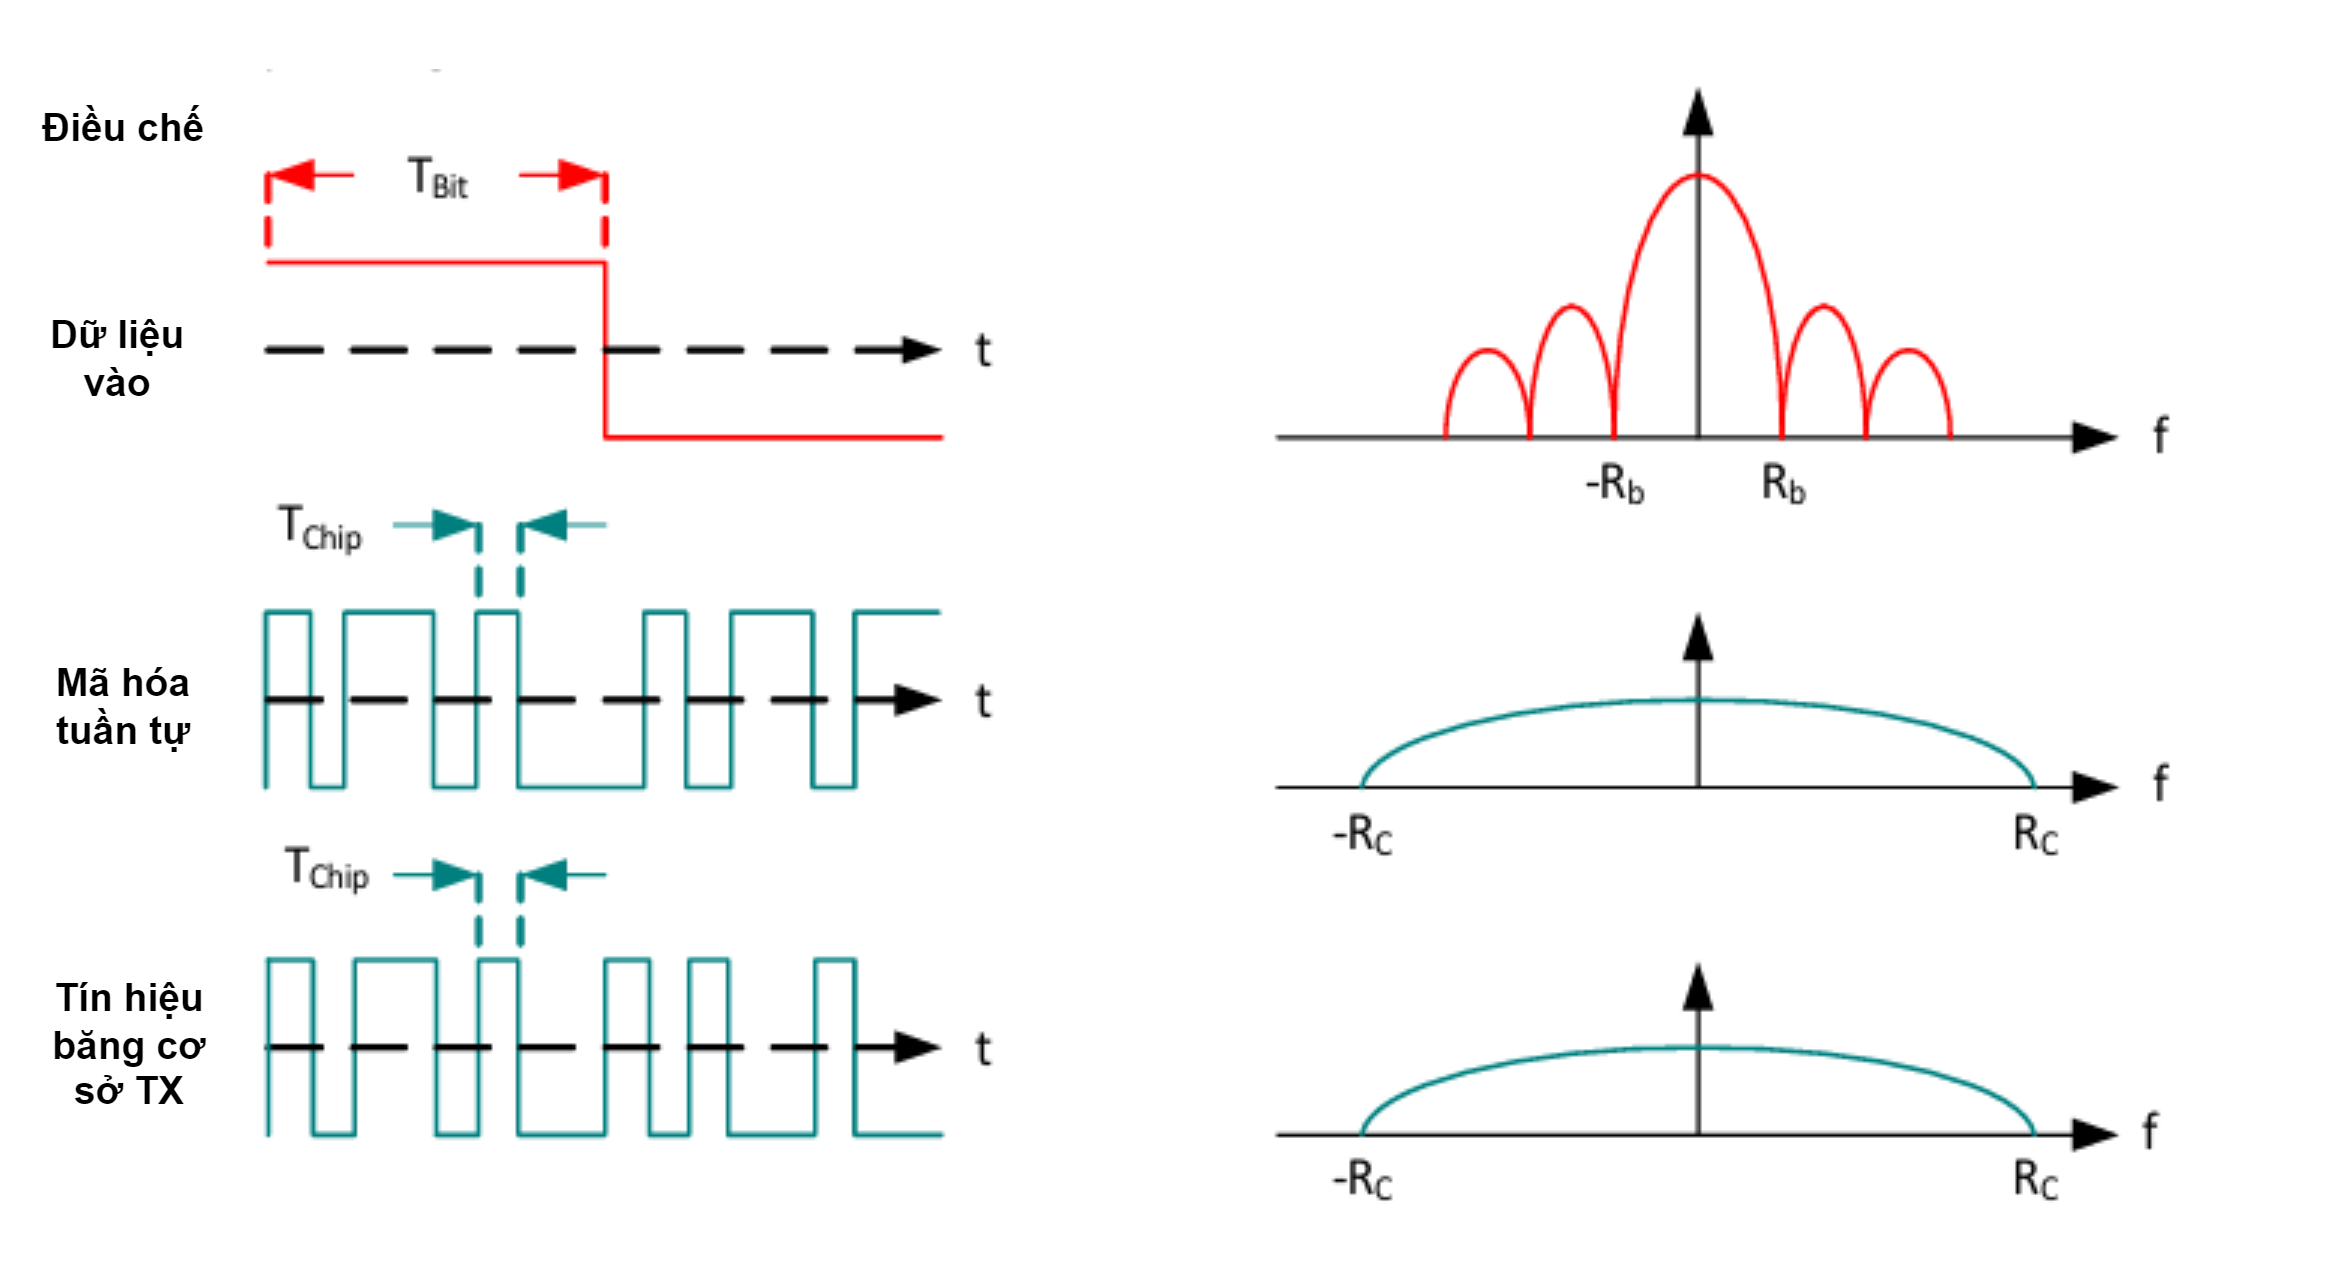
\includegraphics[width=11cm,height=5.4cm]{Images/Traipho.png}
		\caption[Kỹ thuật trải phổ sử dụng chuỗi mã trải phổ \cite{semtech2015an1200}]{\bfseries \fontsize{12pt}{0pt}\selectfont Kỹ thuật trải phổ sử dụng chuỗi mã trải phổ \cite{semtech2015an1200}}
		\label{Traipho}
	\end{figure}
	
	
	Phía máy thu thực hiện tách tín hiệu dữ liệu bằng cách nhân với chuỗi trải phổ một lần nữa Hình \ref{sodotraipho}.
	
	\begin{figure}[!ht]
		\centering
		\includegraphics[width=11cm,height=5.4cm]{Images/sodotraipho.png}
		\caption[Sơ đồ trải phổ \cite{semtech2015an1200}]{\bfseries \fontsize{12pt}{0pt}\selectfont Sơ đồ trải phổ \cite{semtech2015an1200}}
		\label{sodotraipho}
	\end{figure}
	
	\newpage
	Hệ số trải phổ của tín hiệu chip (chip signal) phụ thuộc và tỷ số chip rate và tốc độ dữ liệu yêu cầu (required data rate). Nó được gọi là processing gain, được tính theo công thức \cite{semtech2015an1200}:
	
	\begin{equation}\label{processing_gain}
		G_p=10 \times \log \left(\frac{R_c}{R_b}\right)
	\end{equation}
	Trong đó:
	\begin{itemize}
		\item  $G_p$  (processing gain), đơn vị dB
		\item  $R_c$ là chip rate, đơn vị bps
		\item  $R_b$ là bit yêu cầu (bit rate yêu cầu), đơn vị bps
	\end{itemize}
	
	
	Quá trình này không những tạo ra tín hiệu kháng lại nhiễu kênh truyền mà còn kháng được nhiễu từ các tín hiệu khác. Processing gain cho phép tái xây dựng lại tín hiệu ban đầu chính xác mặc dù SNR có thể âm. Bất kỳ can nhiễu nào cũng dễ dàng được lọc. 
	
	Thách thức lớn nhất của việc triển khai DSSS cho các ứng dụng low-cost và công suất thấp là phải cần có một nguồn xung cực kỳ chính xác. Hơn thế nữa, yêu cầu chip codes dài hơn tốn thời gian giải trải phổ tại máy thu. Nó không những khiến cho máy thu trở nên phức tạp mà lại còn tăng thời gian xử lý ở máy thu. Phía thu phải luôn ở trạng thái đồng bộ với máy phát, nó không thể đáp ứng được với một ứng dụng yêu cầu công suất thấp.
	
	
	\subsubsection{Chirp Spread – Spectrum}
	
	Một chirp là một tín hiệu hình sin tăng dần hoặc giảm dần của tần số theo thời gian Hình \ref{UP_chirp}. Nó dựa trên một tín hiệu chirp tự nhiên cho trải phổ băng thông của tín hiệu gửi. Một chirp tăng dần tần số được gọi là up-chirp được minh hoạ ở hình dưới:
	
	\begin{figure}[!ht]
		\centering
		\includegraphics[width=8cm,height=3.4cm]{Images/Up_chirp.png}
		\caption[Up-chirp trong miền thời gian \cite{zhang2019spread}]{\bfseries \fontsize{12pt}{0pt}\selectfont Up-chirp trong miền thời gian \cite{zhang2019spread}}
		\label{UP_chirp}
	\end{figure}
	
	Một chirp mà tần số giảm dần được gọi là Down-chip Hình \ref{Down_chirp}, được mình hoạ ở hình dưới:
	
	\begin{figure}[!ht]
		\centering
		\includegraphics[width=8cm,height=3.4cm]{Images/Down_Chirp.png}
		\caption[Down-chirp trong miền thời gian \cite{zhang2019spread}]{\bfseries \fontsize{12pt}{0pt}\selectfont Down-chirp trong miền thời gian \cite{zhang2019spread}}
		\label{Down_chirp}
	\end{figure}
	\newpage
	Up-chirp là một chirp có giá trị dương còn down-chirp có giá trị âm. Sự thay đổi tần số có thể là tuyến tính hoặc theo hàm số mũ. Băng thông của một tín hiệu chirp có sự khác biệt giữa tần số đầu tiên và tần số kết thúc.
	
	\paragraph{Nén xung (Pulse Compression)}\mbox{}
	
	Nén xung là một quá trình mà một xung có chu kỳ dài với công suất đỉnh thấp được biến đổi thành một xung có công suất đỉnh lớn và có chu kỳ ngắn. Chirps cho phép thực hiện nén xung rất thẳng bằng tương quan sử dụng một matched filter. Đầu ra của sự tương quan với một matched filter là một xung kết hợp công suất của xung chirp trên chu kỳ hiện tại của nó (Hình \ref{xungchirp}). Kết quả là cho một processing gain lớn và distance resolution.
	
	\begin{figure}[!ht]
		\centering
		\includegraphics[width=9cm,height=4cm]{Images/xungchirp.png}
		\caption[Xung chirp và kết quả xung sau khi nén \cite{zhang2019spread}]{\bfseries \fontsize{12pt}{0pt}\selectfont Xung chirp và kết quả xung sau khi nén \cite{zhang2019spread}}
		\label{xungchirp}
	\end{figure}
	

	\begin{figure}[!ht]
		\centering
		\includegraphics[width=12.5cm,height=4.9cm]{Images/sodokhoiCSS.png}
		\caption[Sơ đồ khối CSS \cite{wang2008performance}]{\bfseries \fontsize{12pt}{0pt}\selectfont Sơ đồ khối CSS \cite{wang2008performance}}
		\label{sodokhoiCSS}
	\end{figure}
	
	Hình trên (Hình \ref{sodokhoiCSS}) mô tả các khối chức năng của hệ thống CSS. Dữ liệu được điều chế sử dụng Up và Down chirp tại máy thu và giải điều chế sử dụng bộ tương quan + matched filter cho nén xung. Nhận lại được các xung nhọn có năng lượng cao dễ dàng cho việc giải mã.	
	
	Đặc tính quan trọng của CSS là khoảng data rate rất lớn. Chirp dựa trên trải phổ có thể dùng để trải tín hiệu cả với miền thời gian và tần số.

	\paragraph{Trải thời gian (Time Spreading)}\mbox{}
	
	Băng thông của tín hiệu chirp chỉ phụ thuộc vào tần số bắt đầu và tấn số kết thúc của chirp, data rate của kỹ thuật điều chế chirp có thể tăng hoặc giảm phụ thuộc vào băng thông. Nên có thể tự do lựa chọn băng thông và tốc độ dữ liệu của tín hiệu mong muốn và điều chỉnh băng thông như yêu cầu. Nó có kết quả với tín hiện mạnh mẽ, tin cậy và băng thông cao.
	
	Hệ thống CSS có nhiều sự khác nhau tuỳ thuộc vào yêu cầu của ứng dụng. Các đặc điểm nổi bật khác bao gồm: chống nhiễu, kháng đa đường, công suất thấp, trễ thấp và CSS không cần đồng bộ. Với những đặc điểm trên CSS đã được phát triển trong chuẩn IEEE 802.15.4.
	
	\subsubsection{LoRa Chirp Spread – Spectrum}
	
	Kỹ thuật điều chế tại LoRa PHY\cite{semtech2015an1200}được phát triển dựa trên CSS truyền thống, kết hợp thêm các đặc điểm của hệ thống DSSS. Tín hiệu LoRa được điều chế sử dụng một tín hiệu chirp tần số biến đổi liên tục. Loại bỏ sự cần thiết có một nguồn xung đồng hồ chính xác và sự đồng bộ tại phía thu. Cả offset tần số và offset thời gian đều tương đương ở cả phía phát và phía thu. Điều này làm cho PHY đơn giản hơn và có khả năng hoạt động yêu cầu công suất thấp và tạo liên kết truyền thông vững chắc, tin cây.
	
	Băng thông của tín hiệu chirp sinh ra cho trải phổ là tương tương với tín hiệu. Bit-rate của điều chế LoRa được định nghĩa bởi công thức\cite{semtech2015an1200}:
	
	\begin{equation} \label{Bit_rate}
		R_b=S F \times \frac{1}{T_s}
	\end{equation}
	
	Trong đó :
	\begin{itemize}
		\item $R_b$ là bit-rate, đơn vị là (bps)
		\item SF là hệ số trải phổ từ 7 – 12Bit
		\item $T_s$  là chu kỳ ký tự (s)
	\end{itemize}
	
	Chu kỳ ký tự được định nghĩa\cite{semtech2015an1200} :
	\begin{equation} \label{Cycle_symbol}
		T_s=\frac{2^{S F}}{B W}
	\end{equation}
	
	Trong đó, BW là băng thông của tín hiệu điều chế (Hz). Theo sự tương quan ở trên, bit-rate và chu kỳ ký tự tỷ lệ nghịch với nhau và tỷ lệ thuận với hệ số trải phổ.
	
	Chip rate của kỹ thuật điều chế LoRa được định nghĩa\cite{semtech2015an1200}:
	\begin{equation} \label{Chip_rate}
		R_c=R_s \times{2^{S F}}
	\end{equation}
	
	Trong đó :
	\begin{itemize}
		\item $R_c$ là chip rate (chips per second)
		\item $R_s$  là symbol rate (symbol per second)
	\end{itemize}
	
	Symbol rate được định nghĩa như sau\cite{semtech2015an1200}:
	\begin{equation} \label{symbol_rate}
		R_s=\frac{1}{T_s}=\frac{B W}{2^{S F}}
	\end{equation}
	nên : 
	
	\begin{equation} 
		R_c=\frac{B W}{2^{S F}} \times 2^{S F}
	\end{equation}
	
	Vậy nên LoRa gửi một chip trên một giây trên một Hertz. Hơn thế nữa, mã sửa sai có chiều dài biến đổi cũng được sử dụng nhằm tăng robustness. Kết quả data rate của kỹ thuật điều chế LoRa như sau\cite{semtech2015an1200}:
	
	\begin{equation}
		R_b=S F \times \frac{\frac{4}{4+C R}}{\frac{2^{S F}}{B W}}    
	\end{equation}
	
	Trong đó:
	\begin{itemize}
		\item CR là coding rate khoảng từ 1 đến 4
		\item SF là hệ số trải phổ khoảng từ 7 – 12
		\item BW là băng thông tín hiệu, thường dùng 125, 250 và 500 kHz.
	\end{itemize}
	
	\subsubsection{Các đặc điểm nổi bật }
	
	\paragraph{Tích tần số - thời gian cao}\mbox{}
	
	Điều chế LoRa có thể tạo nên tích tần số thời gian (bandwidth-time product) lớn hơn 1. Khi có sự kết hợp giữa báo hiệu không đồng bộ, nó khiến tín hiệu LoRa tốt hơn về cả băng tần cũng như băng can nhiễu. Điều chế LoRa có thể xây dựng sự chọn lọc kênh lên đến tới 90 dB và in-band rejection lên tới 20 dB\cite{semtech2015an1200}.
	
	\paragraph{Bandwidth Scalability}\mbox{}
	
	Điều chế LoRa có khả năng đáp ứng cả ứng dụng băng rộng và băng hẹp do vì sự inherent scalability của tần số và băng thông. Module LoRa có thể dễ dàng cấu hình để phù hợp với các loại ứng dụng bằng cách thay đổi các thanh ghi cấu hình
	\cite{semtech2015an1200}.
	
	\paragraph{Mức tiêu thụ năng lượng thấp}\mbox{}
	
	LoRa Modulation thừa kế đặc tính constant envelope của kỹ thuật điều chế FSK, do đó nó có khả năng sử dụng ít năng lượng và hiệu quả ở trạng thái khuếch đại công suất. Hơn thế nữa, processing gain của trải phổ chirp cũng cho phép công suất đầu ra của bộ phát được giảm xuống mà không làm giảm link budget
	\cite{semtech2015an1200}.
	
	\paragraph{Multipath Robostness}\mbox{}
	
	Nhờ sự broadband nature của kỹ thuật trải phổ chirp. LoRa có khả năng chống lại multipath và hiệu ứng fading ở trong môi trường đô thị
	\cite{semtech2015an1200}.
	
	\paragraph{Long Range}\mbox{}
	
	LoRa có khoảng cách truyền thông lớn so với các kỹ thuật như FSK ở cùng mức năng lượng. Khi kết hợp các thuộc tính robustness đã trên trên, link budget của LoRa có thể dịch 4 lần tăng cường ở khoảng cách
	\cite{semtech2015an1200}.
	
	
	\paragraph{Kháng lại hiệu ứng Doppler}\mbox{}
	
	Vì điều chế LoRa là không đồng bộ trong tự nhiên và nó không cần nguồn xung đồng hồ tham chiếu và đồng bộ, dịch tần số có thể loại bỏ hiệu ứng Doppler dễ dàng. Nó khiến cho LoRa có thể ứng dụng trong các ứng dụng có tính di động \cite{semtech2015an1200}.
	\paragraph{Tăng cường dung lượng mạng}\mbox{}
	
	Nhiều tín hiệu trải phổ có thể được truyền đồng thời thông qua kênh khi LoRa sử dụng các hệ số trải phổ trực giao. Tín hiệu sử dụng các hệ số trải phố khác sẽ được lọc như một tín hiệu nhiễu tại máy thu\cite{semtech2015an1200}.
	\paragraph{Đặc điểm về định vị}\mbox{}
	
	LoRa có khả năng phân biệt được giữa lỗi thời gian và tần số, nó cho phép có thể ứng dụng trong các ứng dụng định vị và khoảng cách\cite{semtech2015an1200}.
	
	
	\subsubsection{Các tham số kỹ thuật chính}
	
	Dưới đây là một số tham số đặc trưng, quan trọng nhất của tầng vật lý LoRa\cite{semtech2015an1200}:
	
	\begin{itemize}
		\item Tần số sóng mang (carrier frequency- CF): biểu diễn tần số trung tâm của dải tần số truyền dẫn tín hiệu. Tất cả gồm ba dải tần số được đặc tả trong datasheet SX1278 Semtech.
		\item Băng thông (BW): Là khoảng tần số có khả năng cho tín hiệu truyền qua. Semtech  đưa ra băng tần từ 7.8kHz đến 500kHz. Băng thông lớn cho phép truyền dữ liệu với datarate cao, thời gian trong không gian thấp (time on air) nhưng độ nhạy thu thấp như là kết quả của nhiễu. Những giá trị băng thông hay được sử dụng trong truyền thông LoRa: 125, 250, 500 kHz.
		\item Hệ số trải phổ (SF): biểu thị cho tỷ số chirp (chirp rate) sử dụng để truyền dữ liệu thông qua băng thông khả dụng. Với một SF, thì ta có 2SF chips/symbol. SF thường dùng từ SF6 đến SF12. Với SF12 thì ta có độ nhạy thu và khoảng cách truyền phát là lớn nhất, nhưng tốc độ truyền thấp nhất.
		\item Coding Rate (CR) : được sử dụng trong công nghệ LoRa là một tỷ số sửa lỗi trước (Forward Error Correction FEC rate). Nó cho phép khôi phục lại các bit thông tin bị lỗi do tạp âm. Tỷ số CR cao thì khả năng sửa lỗi cũng tăng nhưng thời gian ngoài không gian (ToA) cũng tăng. Với LoRa, CR có thể là 4/5, 4/6, 4/7 hoặc 4/8.
	\end{itemize}
	
	
	Độ nhạy thu được định nghĩa bởi Semtech\cite{semtech2015an1200}:
	\begin{equation}
		\rho \mathrm{dBm}=-174+\log \mathrm{BW}+\mathrm{NF}+\mathrm{SNR} .
	\end{equation}
	
	Trong đó :
	\begin{itemize}
		\item -174 là nhiễu theo lý thuyết
		\item BW băng thông kênh truyền
		\item NF là hệ số tạp âm máy thu (tùy vào phần cứng)
		\item SNR là tỷ số công suất tín hiệu trên công suất nhiễu
	\end{itemize}
	
	\subsubsection{Thời gian truyền}
	
	Thời gian truyền của bản tin LoRa phụ thuộc vào các tham số chính như BW, CR, SF. Sự kết hợp của ba tham số sẽ cho kết quả thời gian truyền của bản tin có sự khác nhau.
	
	Như công thức tính sysbol-rate $T_s= \frac{1}{R_s}$ , tổng thời gian truyền 1 bản tin của LoRa còn phụ thuộc vào trường mào đầu. Chu kỳ cho một phiên truyền trường mào đầu như sau\cite{mai2020multi} :
	
	
	\begin{equation}
		T_{\text {preamble }}=\left(n_{\text {preamble }}+4.25\right) \times T_s  
	\end{equation}
	
	Trong đó :
	\begin{itemize}
		\item $n_{\text {preamble }}$ là chiều dài trường mào đầu (10 - 65540)
		\item $T_{\text {preamble }}$ là thời gian truyền trường mào đầu
		\item $T_s$ là symbol rate của một preamble
	\end{itemize}
	
	Tương tự, thời gian truyền của payload phụ thuộc vào số lượng ký tự trong payload. Chiều dài ký tự của payload với explicit header được tính như sau\cite{mai2020multi}:
	
	\begin{equation}
		n_{\text {payload }}=8+\max \left(\text { ceil } \frac{(2 P+4 C R C-S F+7)}{(S F-2 D)}(C R+4), 0\right)
	\end{equation}
	
	Và cho implicit header như sau:
	
	\begin{equation}
		n_{\text {payload }}=8+\max \left(\text { ceil } \frac{(2 P+4 C R C-S F+2)}{(S F-2 D)}(C R+4), 0\right)    
	\end{equation}
	
	
	Trong đó :
	\begin{itemize}
		\item SF là hệ số trải phổ được chọn
		\item D = 1 khi tối ưu data rate được bật và ngược lại
		\item CR là coding rate
		\item CRC = 1 khi CRC enable
		\item P là số byte của payload (1 - 255)
	\end{itemize}
	
	Kết quả chu kỳ truyền dẫn như sau :
	\begin{equation}
		T_{\text{payload}}=n_{\text{payload}} \times T_s
	\end{equation}
	
	Tổng thời gian tuyến tính : 
	\begin{equation}
		T_{\text{packet}}=T_{\text{payload}} + T_{\text{preamble}}
	\end{equation}
	
	
	\subsection{Lý thuyết về mạng Mesh }
	\subsubsection{Giới thiệu}
	
	Mạng mesh (hay mạng lưới) là một loại mạng mà trong đó các thiết bị kết nối với nhau không theo một cấu trúc tuyến tính, mà theo một cấu trúc dạng lưới, nơi mỗi nút mạng có thể kết nối trực tiếp, động, và không theo thứ tự với các nút khác. Điều này tạo nên một mạng có khả năng tự phục hồi và tối ưu hóa tuyến đường truyền dữ liệu, đảm bảo kết nối mạnh mẽ và linh hoạt.
	
	\subsubsection{Đặc điểm của cấu trúc liên kết trong mạng Mesh}
	\begin{itemize}
		\item Dự phòng: Cấu trúc liên kết lưới cung cấp mức độ dự phòng cao. Luôn có sẵn các đường dẫn dự phòng cho dữ liệu nếu một liên kết hoặc nút bị lỗi. Sự dư thừa này đảm bảo độ tin cậy của mạng bằng cách giảm khả năng mất dữ liệu hoặc ngừng hoạt động mạng.
		\item Khả năng mở rộng: Mạng lưới có khả năng mở rộng tuyệt vời. Mạng có thể dễ dàng chứa phần cứng hoặc nút mới mà không ảnh hưởng đến kết nối của chúng. Cấu trúc liên kết dạng lưới phù hợp cho các mạng nhỏ và lớn do khả năng mở rộng của nó.
		\item Độ tin cậy: Cấu trúc liên kết dạng lưới là một trong những kiến trúc mạng đáng tin cậy nhất vì tính dự phòng của nó. Nó đảm bảo rằng mạng vẫn có thể hoạt động mặc dù có một số lỗi..
		\item Băng thông cao: Mạng lưới có nhiều kênh để truyền dữ liệu, có thể cung cấp băng thông cao. Điều này khiến chúng trở nên lý tưởng cho các ứng dụng yêu cầu truyền nhiều dữ liệu, chẳng hạn như truyền phát video hoặc xử lý dữ liệu quy mô lớn.
		\item Bảo mật: Cấu trúc liên kết lưới có thể cung cấp bảo mật nâng cao vì dữ liệu có thể được mã hóa và bảo mật tại nhiều điểm khác nhau trong mạng. Sự đa dạng của các trang web truy cập khiến việc truy cập trái phép trở nên khó khăn hơn.
	\end{itemize}
	
	\subsubsection{Cấu Trúc của Mạng Mesh}
	
	Cấu trúc Hình \ref{MeshStructure} liên kết dạng lưới có hai biến thể chính: Mạng Mesh Toàn Phần (Full Mesh Network) và Mạng Mesh Không Toàn Phần (Partial Mesh Network).
	\begin{figure}[!ht]
		\centering
		\includegraphics[width=8cm,height=3.6cm]{Images/MeshStructure.png}
		\caption[Full Mesh Network và Partial Mesh Network \cite{Meshtopology}]{\bfseries \fontsize{12pt}{0pt}\selectfont Full Mesh Network và Partial Mesh Network\cite{Meshtopology}}
		\label{MeshStructure}
	\end{figure}
	\paragraph{Mạng Mesh Toàn Phần (Full Mesh Network)}\mbox{}
	
	Mọi thiết bị hoặc nút trong mạng được chia lưới hoàn toàn được kết nối trực tiếp với mọi thiết bị khác, tạo ra một mạng tương tự như có đường dây điện thoại trực tiếp chạy giữa mỗi người trong phòng. Khả năng kết nối mở rộng mang lại những lợi thế như mức độ dự phòng cao nhất, đảm bảo liên lạc liên tục ngay cả khi một liên kết hoặc nút bị lỗi. Mạng được chia lưới hoàn toàn cũng có độ tin cậy cao do độ trễ thấp do kết nối trực tiếp giữa các thiết bị, khiến chúng trở nên hoàn hảo cho các ứng dụng thời gian thực như chơi game trực tuyến và hội nghị video. Ngoài ra, các mạng này có khả năng mở rộng, giúp việc tích hợp các thiết bị bổ sung trở nên đơn giản bằng cách tạo liên kết trực tiếp đến các nút hiện có. 
	
	\paragraph{Mạng Mesh Không Toàn Phần (Partial Mesh Network)}\mbox{}
	
	Không giống như mạng lưới hoàn toàn, mạng lưới một phần cân bằng giữa kết nối và độ phức tạp. Việc kết nối có chọn lọc các thiết bị trong cấu trúc liên kết dạng lưới một phần giúp giảm nhu cầu sử dụng hệ thống cáp phức tạp và các kết nối vật lý lớn, từ đó giảm chi phí lắp đặt và bảo trì. Phương pháp này đơn giản hóa việc bảo trì và cấu hình mạng, thu hút các doanh nghiệp cỡ trung bình đang tìm kiếm giải pháp thực tế. Mức độ dự phòng của mạng lưới một phần có thể không cao bằng mức độ dự phòng của mạng lưới hoàn toàn, nhưng họ cố tình đặt mức dự phòng khi cần thiết, đảm bảo rằng các đường truyền thông quan trọng là đáng tin cậy mà không gây ảnh hưởng đến mạng.
	
	\subsubsection{Ứng dụng của mạng Mesh}
	Mạng mesh có rất nhiều ứng dụng thực tế trong các lĩnh vực khác nhau, bao gồm:
	
	\begin{itemize}
		\item Nhà Thông Minh (Smart Home): Sử dụng để kết nối các thiết bị IoT trong nhà.
		\item Thành Phố Thông Minh (Smart City): Được triển khai để giám sát và quản lý các hệ thống hạ tầng công cộng như đèn đường, cảm biến chất lượng không khí, và hệ thống giao thông.
		\item Hệ Thống Quản Lý Công Nghiệp (Industrial IoT): Kết nối các thiết bị và cảm biến trong môi trường công nghiệp để giám sát và điều khiển quá trình sản xuất.
		\item Mạng Viễn Thông (Telecommunication): Sử dụng trong các hệ thống viễn thông để cải thiện độ phủ sóng và độ tin cậy của mạng di động.
		\item Thông tin liên lạc trên máy bay: Mạng lưới được sử dụng cho hệ thống thông tin liên lạc trên máy bay. Dự phòng là rất quan trọng để đảm bảo liên lạc liên tục với các trạm mặt đất.
		\item Mạng quân sự: Do tính tin cậy và mạnh mẽ của nó, cấu trúc liên kết dạng lưới thường được sử dụng trong các mạng truyền thông quân sự. Dữ liệu vẫn có thể tìm các tuyến đường thay thế để đến đích ngay cả khi mạng bị gián đoạn do hoạt động thù địch.
	\end{itemize}
	
	
	\subsection{Vi điều khiển}
	\subsubsection{Kiến trúc chung của một vi điều khiển}
	
	\begin{figure}[!ht]
		\centering
		\includegraphics[width=8cm,height=4.5cm]{Images/Armstructure.png}
		\caption[Kiến trúc chung của một vi điều khiển \cite{batatina2021aplikimi}]{\bfseries \fontsize{12pt}{0pt}\selectfont Kiến trúc chung của một vi điều khiển \cite{batatina2021aplikimi}}
		\label{Armstructure}
	\end{figure}
	\newpage
	Hình \ref{Armstructure} cho thấy kiến trúc tổng quát của một vi điều khiển bao gồm các thành phần chính:
	
	\begin{itemize}
		\item CPU : Bộ xử lý trung tâm hay CPU là bộ não của Vi điều khiển. Nó bao gồm Đơn vị logic số học (ALU) và Đơn vị điều khiển (CU). CPU đọc, giải mã và thực thi các hướng dẫn để thực hiện các hoạt động Số học, Logic và Truyền dữ liệu.
		\item Bộ nhớ (MEMORY) : Có hai loại Bộ nhớ: Bộ nhớ chương trình và Bộ nhớ dữ liệu. Bộ nhớ chương trình,chứa chương trình tức là các hướng dẫn được CPU thực thi.  Bộ nhớ dữ liệu được yêu cầu để lưu trữ dữ liệu tạm thời trong khi thực hiện các lệnh.
		\item Cổng đầu vào/ra song song : Giao diện của Bộ vi điều khiển với thế giới bên ngoài được cung cấp bởi Cổng I/O hoặc Cổng đầu vào/đầu ra. Thiết bị đầu vào như Công tắc, Bàn phím, v.v. cung cấp thông tin từ người dùng đến CPU dưới dạng Dữ liệu nhị phân.
		\item Bus : Bus hệ thống là một nhóm dây kết nối CPU với các thiết bị ngoại vi khác như Bộ nhớ, Cổng I/O và các thành phần hỗ trợ khác.
		\item Cổng nối tiếp : Một trong những yêu cầu quan trọng của Vi điều khiển là giao tiếp với các thiết bị và thiết bị ngoại vi khác (bên ngoài). Cổng nối tiếp chứng minh giao diện như vậy thông qua giao tiếp nối tiếp. Giao tiếp nối tiếp phổ biến nhất được triển khai trong Vi điều khiển là UART.
		\item Bộ đếm thời gian và mạch dao động : Một trong những thành phần quan trọng của Vi điều khiển là Bộ định thời và Bộ đếm. Chúng cung cấp các hoạt động Trì hoãn Thời gian và đếm các sự kiện bên ngoài. Ngoài ra, Bộ hẹn giờ và Bộ đếm có thể cung cấp chức năng Tạo, Điều chế độ rộng xung, Điều khiển đồng hồ, v.v.
		\item Bộ chuyển đối analog sang digital (ADC) : Bộ chuyển đổi tương tự sang số hoặc ADC là mạch chuyển đổi tín hiệu Analog thành Tín hiệu số. Mạch ADC tạo thành giao diện giữa các thiết bị Đầu vào tương tự bên ngoài và CPU của Vi điều khiển. Hầu hết tất cả các cảm biến đều là thiết bị tương tự và dữ liệu tương tự từ các cảm biến này phải được chuyển đổi thành dữ liệu số để CPU có thể hiểu được.
		\item Bộ chuyển đối digital sang analog (DAC) : Bộ chuyển đổi kỹ thuật số sang tương tự hoặc DAC là một mạch hoạt động trái ngược với ADC, tức là nó chuyển đổi Tín hiệu số thành Tín hiệu tương tự. DAC tạo thành cầu nối giữa CPU của Vi điều khiển và các thiết bị analog bên ngoài.
		
	\end{itemize}
	
	\subsubsection{Cấu trúc lõi vi xử lý ARM}
	
	ARM (Advanced RISC Machine) là một bộ vi điều khiển tập lệnh rút gọn tiên tiến 32 bits, được giới thiệu bởi tổ chức máy tính Acron vào năm 1987. Là một trong những thiết kế kiến trúc điện tử phổ biến nhất trên thị trường, nó được sử dụng rộng rãi trong các thiết bị điện thoại thông minh, máy tính và những thiết bị điện tử thông thường thậm chí nó còn được sử dụng cho siêu máy tính Fugaku, siêu máy tính nhanh nhất thế giới. Nhờ thiết kế nhỏ gọn, tiết kiện năng lượng và hiệu suất tối ưu.
	
	\begin{figure}[!ht]
		\centering
		\includegraphics[width=8cm,height=4cm]{Images/ARMORIGIN.png}
		\caption[Cấu trúc lõi ARM \cite{ARM}]{\bfseries \fontsize{12pt}{0pt}\selectfont Cấu trúc lõi ARM\cite{ARM}}
		\label{ARM_ORIGIN}
	\end{figure}
	
	Hình \ref{ARM_ORIGIN} là kiến trúc của một lõi ARM gồm các lớp trừu tượng và các thành phần mà các kết nói giao tiếp giữa chúng, trong đó:
	
	\begin{itemize}
		\item WIC : là một bộ điều khiển ngắt được thiết kế để quản lý và phát hiện các tín hiệu ngắt từ các thiết bị ngoại vi hoặc các nguồn ngắt khác khi vi xử lý đang ở trong chế độ tiết kiệm năng lượng, đặc biệt là chế độ ngủ sâu (deep sleep mode).
		\item NVIC (Nest Vector Interrupt Controller): là một điều khiển “on-chip” cung cấp phản hồi có độ trễ nhanh hoặc chậm (tùy theo vai trò của ngắt) tới các sự kiện ngắt trong vi điều khiển.
		\item ARM Core: Là lõi mang kiến trúc ARM.
		\item ETM (Embedded Trace Macrocell): cung cấp cơ sở hạ tầng đầy đủ để gỡ lỗi và theo dõi các bộ vi xử lý lõi ARM, cho phép thu thập thông tin về các chỉ thị đến vi xử lý mà không làm giảm hiệu suất của nó.
		\item DAP (Debug Access Ports) là một cổng gỡ lỗi cho các cổng đầu vào / ra của một vi xử lý, có thể kể đến như JTAG hoặc SW.
		\item Memory protection unit: khối bảo vệ bộ nhớ là một thành phần tự chọn trong vi điều khiển cung cấp quyền truy cập cho vùng nhớ ứng dụng trong hệ thống nhúng.
		\item Serial Wire Viewer: là một tính năng theo dõi dữ liệu phổ biến trên các sản phẩm lõi ARM-Cortex.
		\item Data Watchpoints hay breakpoints: hỗ trợ tạo một sự kiện theo dõi trên phần cứng cho phép tạm dừng chương trình tại một điểm và theo dõi dữ liệu cho đến điểm đó.
		\item Flash Patch: là bộ phận xử lý và triển khai data watchpoints.
		\item Bus matrix: đường bus cho phép kết nối nhiều đường bus AHB, APB và các đường bus bên trong bộ vi xử lý.
		\item Code Interface và SRAM \& Peripheral:  là các ngoại vi và triển khai mã.
	\end{itemize}
	
	\subsubsection{Ưu điểm và nhược điểm của vi điều khiển lõi ARM}
	
	Ưu điểm:
	\begin{itemize}
		\item Bộ xử lý ARM xử lý một bộ xử lý duy nhất mỗi lần, điều này làm cho nó nhanh hơn và tiêu thụ ít năng lượng hơn.
		\item Bộ xử lý ARM hoạt động trong trường hợp hệ thống đa chương trình, nơi sử dụng nhiều bộ xử lý để xử lý thông tin.
		\item Bộ xử lý ARM rẻ hơn so với các bộ xử lý khác, điều này khiến chúng được sử dụng trong điện thoại di động.
		\item Bộ xử lý ARM có khả năng mở rộng, tính năng này giúp nó sử dụng được trên nhiều thiết bị khác nhau.
	\end{itemize}
	
	Nhược điểm:
	
	\begin{itemize}
		\item Bộ xử lý ARM không ổn định so với bộ xử lý x86, và do đó, chúng không thể được sử dụng trong các hệ thống Windows.
		\item Bộ xử lý ARM không có khả năng đạt hiệu suất rất cao, điều này hạn chế chúng trong nhiều ứng dụng.
		\item Thực thi bộ xử lý ARM khá khó, đòi hỏi các lập trình viên có kỹ năng sử dụng nó.
		\item Bộ xử lý ARM không hiệu quả trong việc xử lý các chỉ thị lập lịch (scheduling instructions).
	\end{itemize}
	

	
	\subsection{Chuẩn giao tiếp}
	
	\subsubsection{GPIO}
	
	GPIO là một chân tín hiệu kỹ thuật số trên mạch tích hợp mà hành vi của nó (đầu vào hoặc đầu ra) được điều khiển bởi phần mềm ứng dụng. GPIO về cơ bản là một chân có thể được cấu hình làm đầu vào hoặc đầu ra. Nếu chúng ta cấu hình chân như một đầu ra, chúng ta có thể ghi 0 (LOW) hoặc 3,3 / 5 V (VDD) vào chân đó. 
	
	Khả năng GPIO có thể bao gồm\cite{GPIO}:
	\begin{itemize}
		\item Các chân GPIO có thể được cấu hình để trở thành đầu vào hoặc đầu ra.
		\item Giá trị đầu vào có thể đọc được (thường cao hoặc thấp).
		\item Giá trị đầu ra có thể ghi / đọc được.
		\item Giá trị đầu vào thường có thể được sử dụng làm IRQ (thường cho các sự kiện đánh thức).
	\end{itemize}	
	
	\subsubsection{Giao tiếp I2C}
	I2C (Inter – Integrated Circuit) là 1 giao thức giao tiếp nối tiếp đồng bộ được phát triển bởi Philips Semiconductors, sử dụng để truyền nhận dữ liệu giữa các IC với nhau chỉ sử dụng hai đường truyền tín hiệu.	
	Các bit dữ liệu sẽ được truyền từng bit một theo các khoảng thời gian đều đặn được thiết lập bởi 1 tín hiệu đồng hồ. Bus I2C thường được sử dụng để giao tiếp ngoại vi cho rất nhiều loại IC khác nhau như các loại vi điều khiển, cảm biến, EEPROM.
	
	
	\begin{figure}[!ht]
		\centering
		\includegraphics[width=8cm,height=2.3cm]{Images/I2C.png}
		\caption[Mô hình chuẩn giao tiếp I2C\cite{I2C}]{\bfseries \fontsize{12pt}{0pt}\selectfont Mô hình chuẩn giao tiếp I2C\cite{I2C}}
		\label{i2c}
	\end{figure}
	
	Từ Hình \ref{i2c} cho ta thấy cấu tạo của giao tiếp I2C bao gồm:
	
	\begin{itemize}
		\item I2C sử dụng 2 đường truyền tín hiệu:
		\begin{itemize}
			\item SCL (Serial Clock Line): Tạo xung nhịp đồng hồ do Master phát đi.
			\item SDA (Serial Data Line): Đường truyền nhận dữ liệu.
		\end{itemize}
		\item Giao tiếp I2C bao gồm quá trình truyền nhận dữ liệu giữa các thiết bị chủ tớ, hay Master - Slave.
		\item Thiết bị Master là 1 vi điều khiển, nó có nhiệm vụ điều khiển đường tín hiệu SCL và gửi nhận dữ liệu hay lệnh thông qua đường SDA đến các thiết bị khác.
		\item Các thiết bị nhận các dữ liệu lệnh và tín hiệu từ thiết bị Master được gọi là các thiết bị Slave. Các thiết bị Slave thường là các IC, hoặc thậm chí là vi điều khiển.
		\item Master và Slave được kết nối với nhau như Hình \ref{i2c}. Hai đường bus SCL và SDA đều hoạt động ở chế độ Open Drain, nghĩa là bất cứ thiết bị nào kết nối với mạng I2C này cũng chỉ có thể kéo 2 đường bus này xuống mức thấp (LOW), nhưng lại không thể kéo được lên mức cao. Vì để tránh trường hợp bus vừa bị 1 thiết bị kéo lên mức cao vừa bị 1 thiết bị khác kéo xuống mức thấp gây hiện tượng ngắn mạch. Do đó cần có 1 điện trở (từ 1 -- 4,7 k\(\Omega\)) để giữ mặc định ở mức cao .
	\end{itemize}
	
	
	\subsubsection{Giao tiếp SPI}
	\begin{figure}[!ht]
		\centering
		\includegraphics[width=5cm,height=2.7cm]{Images/SPI.png}
		\caption[Mô hình chuẩn giao tiếp SPI\cite{SPI}]{\bfseries \fontsize{12pt}{0pt}\selectfont Mô hình chuẩn giao tiếp SPI\cite{SPI}}
		\label{SPI}
	\end{figure}
	
	SPI – Serial Peripheral Interface – hay còn gọi là giao diện ngoại vi nối tiếp, được phát triển bởi hãng Motorola. Chuẩn đồng bộ nối truyền dữ liệu ở chế độ full - duplex (hay gọi là "song công toàn phần". Nghĩa là tại 1 thời điểm có thể xảy ra đồng thời quá trình truyền và nhận. 
	
	Là giao tiếp đồng bộ, bất cứ quá trình nào cũng đều được đồng bộ với xung clock sinh ra bởi thiết bị Master nên không cần phải lo lắng về tốc độ truyền dữ liệu.
	
	SPI thường được sử dụng giao tiếp với bộ nhớ EEPROM, RTC (Đồng hồ thời gian thực), IC âm thanh, các loại cảm biến như nhiệt độ và áp suất, thẻ nhớ như MMC hoặc thẻ SD hoặc thậm chí các bộ vi điều khiển khác.
	
	
	Từ Hình \ref{SPI} cho ta thấy cấu tạo của giao thức SPI bao gồm:
	
	\begin{itemize}
		\item MOSI (Master Output Slave Input): Chân này được sử dụng để truyền dữ liệu khi thiết bị được cấu hình là master và là chân nhận dữ liệu khi cấu hình là slave.
		\item MISO (Master Input Slave Output): Chân này được sử dụng để nhận dữ liệu khi khi thiết bị được cấu hình là Master và truyền dữ liệu khi cấu hình bởi slave
		\item SS ( slave select) : Tín hiệu này được tạo bởi Master để lựa chọn thiết bị slave muốn truyền nhận, Đối với thiết bị master chân này được cấu hình là chân xuất (output) và là chân nhập (input) với slave
		\item SCK (serial clock): Chân SCK cấp xung đồng bộ để truyền nhận dữ liệu với một Slave nào đó được chọn.
	\end{itemize}
	
	\subsubsection{Giao tiếp UART}
	UART hay bộ thu-phát không đồng bộ đa năng là một trong những hình thức giao tiếp kỹ thuật số giữa thiết bị với thiết bị đơn giản và lâu đời nhất. Bạn có thể tìm thấy các thiết bị UART trong một phần của mạch tích hợp (IC) hoặc dưới dạng các thành phần riêng lẻ. Các UART giao tiếp giữa hai nút riêng biệt bằng cách sử dụng một cặp dẫn và một nối đất chung.
	\begin{figure}[!ht]
		\centering
		\includegraphics[width=7cm,height=3.3cm]{Images/UART.png}
		\caption[Mô hình chuẩn giao tiếp UART\cite{UART}]{\bfseries \fontsize{12pt}{0pt}\selectfont Mô hình chuẩn giao tiếp UART\cite{UART}}
		\label{uart}
	\end{figure}
	
	Từ Hình \ref{uart} cho ta thấy cấu tạo chuẩn giao tiếp UART bao gồm:
	
	\begin{itemize}
		\item Chân Tx (truyền) của một chip kết nối trực tiếp với chân Rx (nhận) của chip kia và ngược lại. Thông thường, quá trình truyền sẽ diễn ra ở 3.3V hoặc 5V. UART là một giao thức một master, một slave, trong đó một thiết bị được thiết lập để giao tiếp với duy nhất một thiết bị khác.
		\item Dữ liệu truyền đến và đi từ UART song song với thiết bị điều khiển (ví dụ: CPU).
		\item Khi gửi trên chân Tx, UART đầu tiên sẽ dịch thông tin song song này thành nối tiếp và truyền đến thiết bị nhận.
		\item UART thứ hai nhận dữ liệu này trên chân Rx của nó và biến đổi nó trở lại thành song song để giao tiếp với thiết bị điều khiển của nó.
	\end{itemize}
	
	
	Có ba chế độ truyền dữ liệu nối tiếp:
	\begin{itemize}
		\item Full Duplex: Giao tiếp đồng thời đến và đi từ mỗi master và slave
		\item Half Duplex: Dữ liệu đi theo một hướng tại một thời điểm
		\item Simplex: Chỉ giao tiếp một chiều.
	\end{itemize}
	
	
	\subsection{GPS - Global Positioning System}
	\subsubsection{Giới thiệu về GPS}
	Hệ thống định vị toàn cầu ( GPS ) là một hệ thống định vị dựa trên vệ tinh được tạo thành từ một mạng lưới gồm 24 vệ tinh được Bộ Quốc phòng Hoa Kỳ đưa vào quỹ đạo. GPS ban đầu được thiết kế cho các ứng dụng quân sự, nhưng vào những năm 1980, chính phủ đã cung cấp hệ thống này cho mục đích dân sự. GPS hoạt động trong mọi điều kiện thời tiết, mọi nơi trên thế giới, 24 giờ một ngày, 365 ngày một năm. 24 vệ tinh tạo nên phân khúc không gian GPS đang quay quanh trái đất cách chúng ta khoảng 12.000 dặm. Những vệ tinh này đang di chuyển với tốc độ khoảng 7.000 dặm một giờ. Vệ tinh GPS hoạt động bằng năng lượng mặt trời. Chúng có pin dự phòng trên tàu để duy trì hoạt động trong trường hợp nhật thực, khi không có năng lượng mặt trời. Tên lửa đẩy nhỏ trên mỗi vệ tinh giúp chúng bay đúng đường. Mỗi vệ tinh nặng khoảng 2.000 pound và được chế tạo để tồn tại trong khoảng mười năm.
	
	
	\subsubsection{Cách thức hoạt động của GPS}
	
	
	Trong Hình \ref{GPS} các vệ tinh GPS bay vòng quanh trái đất hai lần một ngày theo quỹ đạo rất chính xác và truyền thông tin tín hiệu về trái đất. Bộ thu GPS lấy thông tin này và sử dụng phép đo tam giác để tính toán vị trí chính xác của người dùng. Về cơ bản, máy thu GPS so sánh thời gian tín hiệu được truyền đi bởi vệ tinh với thời gian nhận được. Sự khác biệt về thời gian cho máy thu GPS biết vệ tinh cách bao xa. Giờ đây, với việc đo khoảng cách từ một vài vệ tinh nữa, máy thu có thể xác định vị trí của người dùng và hiển thị nó trên bản đồ điện tử của người dùng. Máy thu GPS phải được khóa vào tín hiệu của ít nhất ba vệ tinh để tính toán vị trí 2D (vĩ độ và kinh độ) và theo dõi chuyển động. Với bốn vệ tinh nữa trong tầm nhìn, máy thu có thể xác định vị trí 3D của người dùng (vĩ độ, kinh độ và độ cao). Khi vị trí của người dùng đã được xác định, thiết bị GPS có thể tính toán các thông tin khác, chẳng hạn như tốc độ, hướng, đường đi, khoảng cách chuyến đi, khoảng cách đến đích, thời gian mặt trời mọc và mặt trời lặn, v.v.
	
	\begin{figure}[!ht]
		\centering
		\includegraphics[width=8cm,height=4.5cm]{Images/GPS.png}
		\caption[Cách thức hoạt động của GPS \cite{GPS} ]{\bfseries \fontsize{12pt}{0pt}\selectfont Cách thức hoạt động của GPS\cite{GPS}}
		\label{GPS}
	\end{figure}	
	
	\subsection{Lý thuyết về hệ điều hành thời gian thực RTOS }
	\subsubsection{Giới thiệu về RTOS}
	Hệ điều hành thời gian thực (RTOS) được áp dụng trong các môi trường có số lượng lớn sự kiện, đa phần xuất hiện từ bên ngoài hệ thống máy tính, yêu cầu phải được tiếp nhận và xử lý trong thời gian ngắn hoặc phải tuân thủ một hạn chế thời gian cụ thể. Các ứng dụng như điều khiển công nghiệp, thiết bị chuyển mạch điện thoại, điều khiển bay và mô phỏng thời gian thực thường sử dụng RTOS. Trong hệ điều hành này, thời gian xử lý được đo bằng phần thập phân của giây. Hệ thống này có một thời hạn cố định và phải hoàn thành xử lý trong các ràng buộc quy định. Nếu không, điều này sẽ dẫn đến hỏng hóc hệ thống.
	
	Hệ điều hành thời gian thực có 2 loại:
	\begin{itemize}
		\item Hệ điều hành thời gian thực cứng (Hard Real-Time) là các hệ điều hành đảm bảo rằng các nhiệm vụ quan trọng phải được hoàn thành trong một khoảng thời gian nhất định. Ví dụ, nếu hệ thống điều khiển của UAV không hoàn thành các tác vụ điều khiển như lập kế hoạch, điều hướng, và thu thập dữ liệu theo đúng thời gian, nó có thể dẫn đến kết quả không mong muốn như mất dữ liệu quan trọng hoặc không thể cung cấp thông tin cần thiết cho người dùng. Đặc biệt trong các tình huống khẩn cấp như tìm kiếm cứu nạn, sự chậm trễ trong việc cung cấp thông tin có thể ảnh hưởng nghiêm trọng đến kết quả cuối cùng.
		\item Hệ điều hành thời gian thực mềm (Soft Real-Time) cung cấp một số sự linh hoạt trong giới hạn thời gian. Ví dụ, các hệ thống đa phương tiện, hệ thống âm thanh kỹ thuật số, v.v. là những ví dụ về hệ điều hành thời gian thực mềm,   ngắt (interrupt).
	\end{itemize}
	
	
	\subsection{Giới thiệu về phần mềm thiết kế 3D}
	\subsubsection{Giới thiệu về Fusion 360}
	Autodesk Fusion 360 như trong Hình \ref{Fusion360} là phần mềm tích hợp thiết kế 3D, sản xuất có hỗ trợ máy tính (CAM), kỹ thuật có hỗ trợ máy tính (CAE) và thiết kế bảng mạch in (PCB) được phát triển bởi Autodesk. Nó được xem là giải pháp "tất cả trong một" cho phép người dùng thiết kế, mô phỏng, sản xuất và quản lý quy trình sản xuất của họ trong một môi trường duy nhất.
	
	\begin{figure}[!ht]
		\centering
		\includegraphics[width=8cm,height=4.2cm]{Images/Fusion360_Logo.png}
		\caption[Phần mềm Fusion 360]{\bfseries \fontsize{12pt}{0pt}\selectfont Phần mềm Fusion 360}
		\label{Fusion360}
	\end{figure}
	
	\subsubsection{Các tính năng của Fusion 360}
	
	\begin{itemize}
		\item Thiết kế 3D mạnh mẽ: Fusion 360 cung cấp một bộ công cụ toàn diện để tạo ra các mô hình 3D phức tạp với độ chính xác cao. Các tính năng bao gồm mô hình hóa tham số, mô hình hóa trực tiếp, mô hình hóa bề mặt và tạo mảng.
		
		\item Sản xuất có hỗ trợ máy tính (CAM): Fusion 360 tích hợp các công cụ CAM mạnh mẽ để lập trình và mô phỏng các quy trình gia công, bao gồm phay, tiện, lập trình CNC, lập trình EDM và in 3D.
		
		\item Kỹ thuật có hỗ trợ máy tính (CAE): Fusion 360 cung cấp các công cụ CAE để mô phỏng hiệu suất của thiết kế trong điều kiện thực tế. Các tính năng bao gồm mô phỏng động lực học, mô phỏng nhiệt và mô phỏng dòng chảy.
		
		\item Thiết kế bảng mạch in (PCB): Fusion 360 cung cấp các công cụ chuyên dụng để thiết kế và bố trí bảng mạch in. Các tính năng bao gồm định tuyến tự động, kiểm tra quy tắc thiết kế và mô phỏng tín hiệu.
		
	\end{itemize}
	
	\subsubsection{Ứng dụng của Fusion 360}
	\begin{itemize}
		\item Kỹ thuật: Fusion 360 được sử dụng rộng rãi trong các ngành kỹ thuật, bao gồm cơ khí, ô tô, hàng không vũ trụ và chế tạo.
		
		\item Sản xuất: Fusion 360 được sử dụng bởi các nhà sản xuất để thiết kế, sản xuất và quản lý quy trình sản xuất của họ.
		
		\item Giáo dục: Fusion 360 được sử dụng trong các trường học và đại học để giảng dạy thiết kế và kỹ thuật.
		
		\item Sử dụng cá nhân: Fusion 360 cũng được sử dụng bởi những người đam mê và nhà sáng tạo để thiết kế và chế tạo các dự án của riêng họ.
		
	\end{itemize}
	\subsection{Kết luận}
	CHƯƠNG 2 là chương tìm hiểu về các cơ sở lý thuyết xoay quanh và cần thiết cho đề tài nghiên cứu. Cơ sở lý thuyết cực kỳ quan trọng, là bước chuẩn bị để có phương pháp tiếp cận, tìm kiếm tài liệu và hướng giải quyết sử dụng cho đề tài một cách hiệu quả và đúng đắn.
	
	
	% CHAPTER 3
	\newpage
	\section*{CHƯƠNG 3. THIẾT KẾ HỆ THỐNG VÀ THỬ NGHIỆM}
	\addcontentsline{toc}{section}{\numberline{}CHƯƠNG 3. THIẾT KẾ HỆ THỐNG VÀ THỬ NGHIỆM}
	\setcounter{section}{3}
	\setcounter{subsection}{0}
	\setcounter{figure}{0}
	\setcounter{table}{0}
	Sau khi tìm hiểu các kiến thức lý thuyết cần thiết liên quan đến đề tài từ CHƯƠNG 2. Chương này em sẽ đưa ra đưa ra chức năng, thiết kế các khối của phần cứng và phần mềm, thử nghiệm sau đó là kết quả đạt được và kết luận.
	
	\subsection{Phân tích hệ thống}
	\subsubsection{Mục đích của hệ thống}
	
	Mục đích của hệ thống là tạo ra mạng cảm biến không dây thu thập dữ liệu các thông số môi trường nước theo thời gian thực từ nhiều bể nuôi tôm. Sau đó giá trị được lưu lại trong thẻ nhớ, hiển thị ngay trên màn hình và được gateway thu lại thông qua lora và gửi lên Cloud thông qua module SIM A7670C. Hệ thống còn có thể hoạt động riêng lẻ khi không có gateway khi tích hợp luôn module SIM A7670C cho node. Hướng đến thiết kế bộ đo gọn nhẹ, dễ lắp đặt và hiệu quả cho quá trình hệ thống hoạt động lâu dài.
	
	\subsubsection{Đối tượng của hệ}
	Đối tượng theo dõi của hệ thống là thông số môi trường nước của tôm chân trắng.
	
	\subsubsection{Yêu cầu chức năng và phi chức năng}
	\paragraph{Yêu cầu chức năng}\mbox{}
	
	\begin{itemize}
		\item  Đối với phần cứng:
		\begin{itemize}[label=$\ast$]
			\item Node có các cảm biến đo thông số môi trường nước pH, DO, EC, nhiệt độ. Dữ liệu từ cảm biến hiển thị ngay tại LCD ở node, lưu trữ dữ liệu qua thẻ nhớ Micro SD, truyền thông qua lora lên gateway thực hiện gửi lên IoT platform server.
			\item Các thông số sẽ được lấy mẫu chuẩn, lưu trữ vào thẻ nhớ và gửi lên IoT platform bằng module SIM A7670C sử dụng giao thức HTTP.
			\item Dữ liệu được truyền lên IoT platform và lưu trữ qua thẻ nhớ được thực hiện mỗi 1 phút một lần.
			\item Tích hợp cảm biến bắt tín hiệu GPS ngay tại điểm đo nhằm quan sát vị trí các node và gateway trên bản đồ thực và tính toán khoảng cách truyền lora hợp lý.
			\item Mạch có khả năng hoạt động riêng lẻ khi không cần gateway. Dữ liệu gửi lên lên IoT platform thông qua module SIM A7670C ngay tại node.
			\item Mạch có khả năng chuyển đổi linh hoạt giữa nguồn adapter và pin.
			\item Màn hình LCD tại node hiển thị tất cả các thông số, thời gian.
			\item Màn hình LCD tại gateway hiển thị thời gian và trạng thái kết nối với lora của node.
			\item Mạch có Adapter để cấp nguồn, có khối xử lý để lọc và phân bố đủ nguồn và dòng cho các khối tác vụ.
			\item Mỗi node đều có sử dụng pin trong trường hợp mất điện.
			\item Tích hợp mạch sạc năng lượng mặt trời vào trong khối nguồn của node trong thời điểm mất điện lâu dài.
			\item Khối thời gian thực sử dụng thạch anh nội để hiển thị thời gian, ngày, tháng và năm hiện tại.
		\end{itemize}
		
		\item Đối với phần mềm:
		\begin{itemize}[label=$\ast$]
			\item Sử dụng IoT platform, có thể đặt thủ công vị trí hiện tại của nút cảm biến, hiển thị dòng dữ liệu theo thời gian gửi lên.
			\item Xử lý được các task vụ đa node, đảm bảo hiện thị được đúng các yêu cầu của đầu ra đối với những trường hợp riêng biệt khi truyền nhận dữ liệu.
		\end{itemize}
	\end{itemize}
	\paragraph{Yêu cầu phi chức năng}\mbox{}
	\begin{itemize}
		
		
		\item Đối với phần cứng:
		\begin{itemize}[label=$\ast$]
			\item Sử dụng ESP32 S3
			\item Sử dụng module SIM A7670C
			\item Sử dụng thẻ nhớ Micro SD
			\item Nguồn sử dụng 12V, 4A
			\item Sử dụng mạch sạc năng lượng mặt trời và tấm pin mặt trời 12V, 5W
			\item Sử dụng module GPS ATGM336H
			\item Sử dụng các module cảm biến khói và bụi
			\item Sử dụng module ADS1115
			\item Sử dụng module Lora sx1278
			\item Sử dụng module DS3231
			\item Sử dụng TFT LCD để hiển thị các thông số cảm biến
			\item Hộp đựng mạch được thiết kế 3D.
			\item Chi phí dự kiến nhỏ hơn 2.000.000 VNĐ.
			\item Mainboard được thiết kế và hàn trực tiếp.
		\end{itemize}
		
		\item Đối với phần mềm:
		\begin{itemize}[label=$\ast$]
			\item Sử dụng ngôn ngữ lập trình C và phần mềm Esp-idf cho phần cứng.
			\item Vẽ mạch in bằng phần mềm Altium designer.
			\item Vẽ hộp dựng bằng phần mềm Fusion 360.
			\item Sử dụng nền tảng dữ liệu IOT.
		\end{itemize}
	\end{itemize}
	
	\subsection{Thiết kế hệ thống}
	\subsubsection{Thiết kế mạch cứng của hệ thống}
	\paragraph{Tổng quan phần cứng}\mbox{}
	
	Hệ thống thiết kế 2 thiết bị đó là Node và Gateway.
	
	\begin{itemize}[label=$\ast$]
		\item Đối với thiết bị Node: Đọc dữ liệu từ cảm biến sau đó gửi dữ liệu lên Gateway.
		\item Đối với thiết bị Gateway: Nhận dữ liệu từ phía Node và gửi dữ liệu lên Server.
	\end{itemize}
	
	\begin{itemize}
		\item  Sơ đồ khối phần cứng của node gồm có 9 khối như Hình \ref{Node}:
		
		\begin{figure}[!ht]
			\centering
			\includegraphics[width=9cm,height=5cm]{Images/Node.png}
			\caption[Sơ đồ khối hệ thống Node]{\bfseries \fontsize{12pt}{0pt}\selectfont Sơ đồ khối hệ thống Node}
			\label{Node}
		\end{figure}
		
		\begin{itemize}[label=$\ast$]
			\item Khối nguồn: Sử dụng Adapter 12V – 3A, pin Lithium 2700mAh.
			\item Khối xử lý: Sử dụng hai vi điều khiển ESP32 S3 để xử lý tín hiệu từ khối cảm biến, khối GPS, khối thời gian thực, lưu trữ và gửi dữ liệu qua khối truyền thông và khối hiển thị.
			\item Khối cảm biến: Sử dụng các cảm biến nhiệt độ, pH, DO, EC để nhận thông tin các thông số từ môi trường.
			\item Khối hiển thị: Sử dụng màn hình TFT LCD để hiển thị các thông số đo được từ môi trường, thời gian thực.
			\item Khối thời gian thực: Thực hiện cung cấp cho bộ đo thời gian sát với thời gian thực bên ngoài.
			\item Khối GPS: Thu tín hiệu GPS từ vệ tinh, lấy được vị trí tại nơi đặt bộ đo.
			\item Khối lưu trữ: Thực hiện lưu trữ bằng microSD các giá trị cảm biến, thời gian, vị trí tránh tình trạng mất dữ liệu nếu mất kết nối tới khối truyền thông.
			\item Khối truyền thông: Sử dụng module Lora để truyền thông về gateway, bên cạnh đó sử dụng Module sim để truyền dữ liệu đã thu thập được lên IoT platform server trong trường hợp không tích hợp gateway hoặc mất kết nối tới Lora bên gateway.
		\end{itemize}
		
		\item Sơ đồ khối phần cứng của gateway gồm có 6 khối như Hình \ref{Gateway}:
		\begin{figure}[!ht]
			\centering
			\includegraphics[width=9cm,height=5cm]{Images/Gateway.png}
			\caption[Sơ đồ khối hệ thống Gateway]{\bfseries \fontsize{12pt}{0pt}\selectfont Sơ đồ khối hệ thống Gateway}
			\label{Gateway}
		\end{figure}
		
		\begin{itemize}[label=$\ast$]
			\item Khối nguồn: Sử dụng Adapter 5V – 2A.
			\item Khối xử lý: Sử dụng vi điều khiển ESP32 S3 để xử lý tín hiệu từ khối truyền thông, khối GPS và gửi dữ liệu lên IoT platform server và khối hiển thị.
			\item Khối hiển thị: Sử dụng màn hình TFT LCD để hiển thị thời gian và trạng thái kết nối tới các node.
			\item Khối thời gian thực: Thực hiện cung cấp cho bộ đo thời gian sát với thời gian thực bên ngoài.
			\item Khối GPS: Thu tín hiệu GPS từ vệ tinh, lấy được vị trí tại nơi đặt gateway.
			\item Khối truyền thông: Sử dụng module Lora để nhận tín hiệu từ node, dữ liệu sẽ được Module sim truyền lên IoT platform server.
		\end{itemize}
	\end{itemize} 
	\paragraph{Chi tiết các khối}\mbox{}
	\begin{itemize}
		
		\item  Khối vi xử lý
		
		Sử dụng vi điều khiển ESP32S3 
		\begin{figure}[!ht]
			\centering
			\includegraphics[width=4.2cm,height=5cm]{Images/ESP32S3.png}
			\caption[Vi điều khiển ESP32 S3\cite{esp32s3} ]{\bfseries \fontsize{12pt}{0pt}\selectfont Vi điều khiển ESP32 S3\cite{esp32s3} }
			\label{ESP32S3}
		\end{figure}
		
		\begin{table}[H]
			\centering
			\begin{tabular}{|l|l|l}
				\cline{1-2}
				\textbf{Đặc điểm}            & \textbf{Thông số}                                                                                      &  \\ \cline{1-2}
				Tần số hoạt động             & 2.                                                                                                     &  \\ \cline{1-2}
				Công suất phát ra            & 20.5dBm                                                                                                &  \\ \cline{1-2}
				Điện áp cung cấp             & \begin{tabular}[c]{@{}l@{}}Tối thiểu: 3V\\ Tối đa: 3.6V\end{tabular}                                   &  \\ \cline{1-2}
				Loại giao diện               & GPIO,I2C,I2S,SPI,UART                                                                                  &  \\ \cline{1-2}
				Nhiệt độ hoạt động tối thiểu & $-40^\circ$C,$+85^\circ$C                                                                                              &  \\ \cline{1-2}
				Giao thức                    & \begin{tabular}[c]{@{}l@{}}Bluetooth, BLE - 802.15.1: Bluetooth 5.0\\ WiFi - 802.11: WiFi\end{tabular} &  \\ \cline{1-2}
				Tốc độ dữ liệu               & 150 Mb/s                                                                                               &  \\ \cline{1-2}
			\end{tabular}
			\caption[Thông số kỹ thuật ESP32S3\cite{esp32s3}]{\bfseries\fontsize{12pt}{0pt}\selectfont Thông số kỹ thuật ESP32S3\cite{esp32s3}}
			\label{ThongsoESP32S3}
		\end{table}
		
		Hình \ref{ESP32S3} và Bảng \ref{ThongsoESP32S3} là hình ảnh và thông số kỹ thuật của vi điều khiển được sử dụng trong đồ án, gồm 3 vi điều khiển ESP32S3 với 2 cho Node và 1 cho Gateway, chi tiết 2 tác vụ xem tại mục 3.2.2.1 và 3.2.2.2.
		
		\item Khối cảm biến 
		\begin{itemize}[label=$\ast$]
			\item Cảm biến nhiệt độ: 
			
			
			\begin{figure}[!ht]
				\centering
				\includegraphics[width=5cm,height=5cm]{Images/temp.png}
				\caption[Cảm biến nhiệt độ NTC 10k$\Omega$\cite{ntcdata}]{\bfseries \fontsize{12pt}{0pt}\selectfont Cảm biến nhiệt độ NTC 10k$\Omega$\cite{ntcdata}}
				\label{Temp}
			\end{figure}
			\begin{table}[H]
				\centering
				\begin{tabular}{|l|l|l}
					\cline{1-2}
					\textbf{Đặc điểm}   & \textbf{Thông số} &  \\ \cline{1-2}
					Phạm vi cảm biến    & -20°C đến 105°C     &  \\ \cline{1-2}
					Loại cảm            & Cảm biến analog   &  \\ \cline{1-2}
					Hằng số B           & 3380              &  \\ \cline{1-2}
					Nhiệt độ tại 10k$\Omega$ & 25°C              &  \\ \cline{1-2}
				\end{tabular}
				\caption[Thông số kỹ thuật NTC 10k$\Omega$\cite{ntcdata}]{\bfseries\fontsize{12pt}{0pt}\selectfont Thông số kỹ thuật NTC 10k$\Omega$\cite{ntcdata}}
				\label{TempTable}
			\end{table}
			Hình \ref{Temp} và Bảng \ref{TempTable} là hình ảnh và thông số kỹ thuật của cảm biến NTC 10k$\Omega$ được sử dụng trong đồ án nhằm thu thập dữ liệu nhiệt độ.
			
			\item Cảm biến pH:
			\begin{figure}[!ht]
				\centering
				\includegraphics[width=5cm,height=5cm]{Images/PH.png}
				\caption[Cảm biến pH\cite{pHDF}]{\bfseries \fontsize{12pt}{0pt}\selectfont Cảm biến pH\cite{pHDF}}
				\label{PHImage}
			\end{figure}
			
			
			\begin{table}[H]
				\centering
				\begin{tabular}{|l|l|}
					\hline
					\textbf{Đặc điểm} & \textbf{Thông số} \\ \hline
					Điện áp cung cấp  & 5.0V              \\ \hline
					Phạm vi           & 0 -14 pH          \\ \hline
					Độ chính xác      & ± 0,1 pH (25 °C)  \\ \hline
					Đầu nối           & BNC               \\ \hline
					Đo nhiệt độ       & 0 - 60°C          \\ \hline
				\end{tabular}
				\caption[Thông số kỹ thuật cảm biến pH\cite{pHDF}]{\bfseries\fontsize{12pt}{0pt}\selectfont Thông số kỹ thuật cảm biến pH\cite{pHDF}}
				\label{ThongsopH}
			\end{table}
			Hình \ref{PHImage} và Bảng \ref{ThongsopH} là hình ảnh và thông số kỹ thuật của cảm biến pH được sử dụng trong đồ án nhằm thu thập dữ liệu thông số pH.
			
			\item Cảm biến EC : 
			
			\begin{figure}[!ht]
				\centering
				\includegraphics[width=5cm,height=4.3cm]{Images/ECSensor.png}
				\caption[Cảm biến EC\cite{ECDF}]{\bfseries \fontsize{12pt}{0pt}\selectfont Cảm biến EC\cite{ECDF}}
				\label{ECSensor}
			\end{figure}
			
			\begin{table}[H]
				\centering
				\begin{tabular}{|l|l|}
					\hline
					Đặc điểm         & Thông số      \\ \hline
					Điện áp cung cấp & 3.0 - 5.0V    \\ \hline
					Điện áp đầu ra   & 0 – 3.2V      \\ \hline
					Phạm vi          & 10 – 100ms/cm \\ \hline
					Độ chính xác     & ± 5\% FS      \\ \hline
					Phạm vi nhiệt độ & 0 - 40°C      \\ \hline
				\end{tabular}
				\caption[Thông số kỹ thuật cảm biến EC\cite{ECDF}]{\bfseries\fontsize{12pt}{0pt}\selectfont Thông số kỹ thuật cảm biến EC\cite{ECDF}}
				\label{ThongsoEC}
			\end{table}
			Hình \ref{ECSensor} và Bảng \ref{ThongsoEC} là hình ảnh và thông số kỹ thuật của cảm biến EC được sử dụng trong đồ án nhằm thu thập dữ liệu cho hai thông số độ đẫn điện.
			
			\item Cảm biến DO:
			\begin{figure}[!ht]
				\centering
				\includegraphics[width=7cm,height=3.6cm]{Images/DOsensor.png}
				\caption[Cảm biến DO\cite{DODF}]{\bfseries \fontsize{12pt}{0pt}\selectfont Cảm biến DO\cite{DODF}}
				\label{DOsensor}
			\end{figure}
			\begin{table}[H]
				\centering
				\begin{tabular}{|l|l|}
					\hline
					Đặc điểm         & Thông số    \\ \hline
					Điện áp cung cấp & 3.3 - 5.5V  \\ \hline
					Điện áp đầu ra   & 0 – 3V      \\ \hline
					Phạm vi          & 0 – 20 mg/L \\ \hline
					Kiểu đầu dò      & BNC         \\ \hline
					Phạm vi nhiệt độ & 0 - 40°C    \\ \hline
				\end{tabular}
				\caption[Thông số kỹ thuật cảm biến DO\cite{DODF}]{\bfseries\fontsize{12pt}{0pt}\selectfont Thông số kỹ thuật cảm biến DO\cite{DODF}}
				\label{ThongsoDO}
			\end{table}
			Hình \ref{DOsensor} và Bảng \ref{ThongsoDO} là hình ảnh thông số kỹ thuật của cảm biến DO sử dụng trong đồ án thu thập dữ liệu thông nồng độ oxy hòa tan trong nước.
			
			\item Khối hiển thị:
			\begin{itemize}
				\item[\ding{70}] Sử dụng module TFT LCD 1.8 inches cho \textbf{Node}.
				\begin{figure}[!ht]
					\centering
					\includegraphics[width=5cm,height=3.5cm]{Images/LCD1.8.png}
					\caption[TFT LCD 1.8 inches\cite{TFT1.8}]{\bfseries \fontsize{12pt}{0pt}\selectfont TFT LCD 1.8 inches\cite{TFT1.8}}
					\label{LCD1.8}
				\end{figure}
				\begin{table}[H]
					\centering
					\begin{tabular}{|l|l|}
						\hline
						Đặc điểm           & Thông số         \\ \hline
						Điện áp cung cấp   & 3.3 – 5V         \\ \hline
						Kích cỡ màn hình   & 1.8 inch         \\ \hline
						Độ phân giải       & 128 x 160 pixels \\ \hline
						IC Driver hiển thị & ST7735           \\ \hline
					\end{tabular}
					\caption[Thông số kỹ thuật TFT LCD 1.8 inches\cite{TFT1.8}]{\bfseries\fontsize{12pt}{0pt}\selectfont Thông số kỹ thuật TFT LCD 1.8 inches\cite{TFT1.8}}
					\label{ThongsoLCD1.8}
				\end{table}
				Hình \ref{LCD1.8} và Bảng \ref{ThongsoLCD1.8} là hình ảnh và thông số kỹ thuật của màn hình LCD có màu được sử dụng trong node nhằm hiển thị các thông số thu thập được từ cảm biến.
				\item[\ding{70}] Sử dụng module TFT LCD 3.5 inches cho \textbf{Gateway}
				
				\begin{figure}[!ht]
					\centering
					\includegraphics[width=6cm,height=3.5cm]{Images/LCD3.5.png}
					\caption[TFT LCD  3.5 inches\cite{TFT3.5}]{\bfseries \fontsize{12pt}{0pt}\selectfont TFT LCD  3.5 inches\cite{TFT3.5}}
					\label{LCD3.5}
				\end{figure}
				\begin{table}[H]
					\centering
					\begin{tabular}{|l|l|}
						\hline
						Đặc điểm           & Thông số         \\ \hline
						Điện áp cung cấp   & 3.3 – 5V         \\ \hline
						Kích cỡ màn hình   & 3.5 inches       \\ \hline
						Độ phân giải       & 320 x 480 pixels \\ \hline
						IC Driver hiển thị & ILI9486          \\ \hline
					\end{tabular}
					\caption[Thông số kỹ thuật TFT LCD 3.5 inches\cite{TFT3.5}]{\bfseries\fontsize{12pt}{0pt}\selectfont Thông số kỹ thuật TFT LCD 3.5 inches\cite{TFT3.5}}
					\label{ThongsoLCD3.5}
				\end{table}
				Hình \ref{LCD3.5} và Bảng \ref{ThongsoLCD3.5} là hình ảnh và thông số kỹ thuật của màn hình LCD có màu được sử dụng trong gateway nhằm hiển thị trạng thái kết nối.
			\end{itemize}
			
		\end{itemize}
		\item Khối truyền thông
		\begin{itemize}[label=$\ast$]
			\item Module sim A7670C
			\begin{figure}[!ht]
				\centering
				\includegraphics[width=4cm,height=4cm]{Images/A7670C.png}
				\caption[Module Sim 7670C\cite{a7670c}]{\bfseries \fontsize{12pt}{0pt}\selectfont Module Sim 7670C\cite{a7670c}}
				\label{A7670C}
			\end{figure}
			\begin{table}[H]
				\centering
				\begin{tabular}{|l|l|}
					\hline
					Đặc điểm                                               & Thông số                     \\ \hline
					Module lõi                                             & A7670C-FASL                  \\ \hline
					Mạng sử dụng                                           & 4G Cat.1 + GSM               \\ \hline
					Điện áp hoạt động                                      & 3.8V                         \\ \hline
					Mức logic I/O                                          & TTL (Serial 3.3V)            \\ \hline
					\multicolumn{1}{|c|}{\multirow{3}{*}{Băng tần hỗ trợ}} & -LTE-TDD B34/B38/B39/B40/B41 \\ \cline{2-2} 
					\multicolumn{1}{|c|}{}                                 & - LTE-FDD B1/B3/B5/B8        \\ \cline{2-2} 
					\multicolumn{1}{|c|}{}                                 & - GSM/GPRS: 900/1800Mhz      \\ \hline
					\multirow{2}{*}{Tốc độ}                                & - LTE(Mbps): 10(DL)/5(UL)    \\ \cline{2-2} 
					& - GSM/GPRS(Kbps):85.6/85.6   \\ \hline
					\multirow{2}{*}{Giao thức hỗ trợ}                      & TCP/IP/IPV4/IPV6/Multi-PDP   \\ \cline{2-2} 
					& FTP/FTPS/HTTP/HTTPS/DNS      \\ \hline
				\end{tabular}
				\caption[Thông số kỹ thuật Module SIM 7670C]{\bfseries\fontsize{12pt}{0pt}\selectfont Thông số kỹ thuật Module SIM 7670C}
				\label{BANGA7670C}
			\end{table}
			Hình \ref{A7670C} và Bảng \ref{BANGA7670C} là hình ảnh và thông số kỹ thuật của module SIM 7670C được sử dụng trong đồ án đóng vai trò cho tác vụ truyền thông, gửi bản tin chứa dữ liệu của các cảm biến đến IoT platform.
			\item Module Lora sx1278
			\begin{figure}[!ht]
				\centering
				\includegraphics[width=4cm,height=3.7cm]{Images/Sx1278.png}
				\caption[Module Lora sx1278\cite{SX1278}]{\bfseries \fontsize{12pt}{0pt}\selectfont Module Lora sx1278 \cite{SX1278}}
				\label{Sx1278}
			\end{figure}
			
			\begin{table}[H]
				\centering
				\begin{tabular}{|l|l|}
					\hline
					Đặc điểm                 & Thông số                                             \\ \hline
					Điện áp hoạt động        & 2.5V - 3.7V                                          \\ \hline
					Dòng điện hoạt động gửi  & 120mA                                                \\ \hline
					Dòng điện hoạt động nhận & 10.8mA                                               \\ \hline
					Dòng ở chế độ chờ        & 0.2uA                                                \\ \hline
					Công suất                & 600mW                                                \\ \hline
					Chuẩn truyền             & SPI                                                  \\ \hline
					Điều chế                 & FSK,GFSK,MSK,GMSK,LoRaTM,OOK\\ \hline
					Nhiệt độ hoạt động       & -40°C – 85°C                                         \\ \hline
					Độ nhạy                  & +20dBm – 10dBm                                       \\ \hline
					Tần số                   & 420 – 450Mhz                                         \\ \hline
					Công suất                & 20dbm (100mW)                                        \\ \hline
					Khoảng cách              & 8000m                                                \\ \hline
					Tốc độ truyền            & 300Kbps (mặc định 2.4 Kbps)                          \\ \hline
				\end{tabular}
				\caption[Thông số kỹ thuật Module Lora sx1278\cite{SX1278}]{\bfseries\fontsize{12pt}{0pt}\selectfont Thông số kỹ thuật Module Lora sx1278\cite{SX1278}}
				\label{TsSx1278}
			\end{table}
			Hình \ref{Sx1278} và Bảng \ref{TsSx1278} là hình ảnh và thông số kỹ thuật của module Lora sx1278 được sử dụng trong đồ án đóng vai trò cho tác vụ truyền thông chính giữa các Node và Gateway.
		\end{itemize}
		\item  Khối nguồn
		Đối với việc dùng pin  năng lượng mặt trời, để cung cấp điện áp và dòng liên tục cho pin và vào vệ trong quá trình sạc và xả pin IC CN3795 đáp ứng.
		\begin{figure}[!ht]
			\centering
			\includegraphics[width=4cm,height=3.6cm]{Images/CN3795.png}
			\caption[IC CN3795\cite{ICCN3795}]{\bfseries \fontsize{12pt}{0pt}\selectfont IC CN3795\cite{ICCN3795}}
			\label{CN3795}
		\end{figure}
		\begin{table}[H]
			\centering
			\begin{tabular}{|l|l|}
				\hline
				Đặc điểm                & Thông số   \\ \hline
				Nguồn cấp               & 6.6 – 30V  \\ \hline
				Điện áp điều chỉnh MPPT & 1.205V     \\ \hline
				Ngưỡng chế độ ngủ       & 0.05V      \\ \hline
				Ngưỡng thoát chế độ ngủ & 0.32V      \\ \hline
				Ngưỡng sạc lại          & 58.8\% Icc \\ \hline
				Ngưỡng kết thúc sạc     & 16\% Icc   \\ \hline
				Tần số chuyển mạch PWM  & 310kHz     \\ \hline
				Dòng sạc tối đa         & 4A         \\ \hline
				Dòng tiêu thụ           & 1mA        \\ \hline
			\end{tabular}
			\caption[Thông số kỹ thuật IC CN3795\cite{ICCN3795} ]{\bfseries\fontsize{12pt}{0pt}\selectfont Thông số kỹ thuật IC CN3795\cite{ICCN3795}}
			\label{ICCN3795}
		\end{table}
		
		CN3795 là bộ điều khiển sạc pin đa hóa chất chế độ chuyển mạch PWM có thể được cung cấp năng lượng bởi tế bào quang điện với chức năng theo dõi điểm công suất tối đa (MPPT) sử dụng một số ít các thành phần bên ngoài. CN3795 được thiết kế đặc biệt để sạc pin lithium ion, LiFePO4 hoặc Lithium Titanate với chế độ dòng điện không đổi và điện áp không đổi.
		
		Các pin bị xả sâu sẽ tự động được sạc nhỏ giọt ở mức 17,5 \% của dòng sạc không đổi đã lập trình cho đến khi điện áp của tế bào vượt quá 66,5\% điện áp không đổi. Chu kỳ sạc kết thúc khi dòng sạc giảm xuống còn 16\% của dòng điện toàn thang, và một chu kỳ sạc mới tự động bắt đầu nếu dòng sạc tăng lên trên 58,8\% của dòng sạc toàn thang. Đặc biệt CN3795 sẽ tự động chuyển sang chế độ ngủ khi điện áp đầu vào thấp hơn điện áp pin khi đó sẽ dừng việc sạc cho pin khi không còn đủ quang năng để sạc cho pin. 
		
		Để có thể linh hoạt chuyển đổi giữa 2 nguồn là pin và adapter, sử dụng rơle 5V.
		
		\begin{figure}[!ht]
			\centering
			\includegraphics[width=4cm,height=3.6cm]{Images/Relay.png}
			\caption[Module Relay\cite{relay}]{\bfseries \fontsize{12pt}{0pt}\selectfont Module Relay\cite{relay}}
			\label{Relay}
		\end{figure}
		
		\begin{table}[H]
			\centering
			\begin{tabular}{|l|l|}
				\hline
				Đặc điểm            & Thông số      \\ \hline
				Điện áp kích hoạt   & 5V            \\ \hline
				Dòng điện danh định & 70mA          \\ \hline
				Dòng tải DC tối đa  & 10A           \\ \hline
				Chuyển đổi tối đa   & 200 lần /phút \\ \hline
				Thời gian hoạt động & 5 miligiây    \\ \hline
				Nguồn cấp           & 6.6 – 30V     \\ \hline
			\end{tabular}
			\caption[Thông số kỹ thuật Relay\cite{relay}]{\bfseries\fontsize{12pt}{0pt}\selectfont Thông số kỹ thuật Relay\cite{relay}}
			\label{TsRelay}
		\end{table}
		
		Hình \ref{Relay} và Bảng \ref{TsRelay} là hình ảnh và thông số kỹ thuật của Rơle 5V được sử dụng chuyển đổi linh hoạt giữa 2 nguồn Adater và pin giúp cho mạch hoạt động liên tục tránh trường hợp bị ngắt khi mất điện lưới.
		
		\item Khối GPS
		\begin{figure}[!ht]
			\centering
			\includegraphics[width=3.6cm,height=3.6cm]{Images/GPSModule.png}
			\caption[Module GPS atgm336h5\cite{GPS_mol}]{\bfseries \fontsize{12pt}{0pt}\selectfont Module GPS atgm336h\cite{GPS_mol}}
			\label{GPSModule}
		\end{figure}
		\begin{table}[H]
			\centering
			\begin{tabular}{|l|l|}
				\hline
				Đặc điểm                  & Thông số        \\ \hline
				Nguồn cấp                 & 2.7 – 3.6V      \\ \hline
				Độ nhạy khi khởi động     & -148dBm         \\ \hline
				Độ nhạy khi theo dõi      & -162dBm         \\ \hline
				Độ chính xác định vị      & 2.5m (CEP50)    \\ \hline
				Thời gian định vị lần đầu & 32s             \\ \hline
				Dòng tiêu thụ             & $<$25mA \\ \hline
			\end{tabular}
			\caption[Thông số kỹ thuật GPS\cite{GPS}]{\bfseries\fontsize{12pt}{0pt}\selectfont Thông số kỹ thuật GPS\cite{GPS}}
			\label{TsGPS}
		\end{table}
		
		Hình \ref{GPSModule} và Bảng \ref{TsGPS} là hình ảnh và thông số kỹ thuật của module GPS atgm336h được sử dụng trong đồ án đóng vai trò cho cung cấp vị trí hệ thống.
	\end{itemize}
	\paragraph{Thiết kế mạch}\mbox{}
	
	\begin{itemize}
		
		
		\item Khối nguồn
		\begin{table}[H]
			\centering
			\begin{tabular}{|l|l|l|}
				\hline
				Khối chức năng      & Yêu cầu nguồn đầu vào & IC nguồn sử dụng       \\ \hline
				Khối vi xử lý       & 3.3V                  & AMS1117 3.3V           \\ \hline
				Khối GPS            & 3.3V                  & AMS1117 3.3V           \\ \hline
				Khối thời gian thực & 3.3V                  & AMS1117 3.3V           \\ \hline
				Khối hiển thị       & 5V                    & MP1584EN               \\ \hline
				Khối thẻ nhớ SD     & 3.3V                  & AMS1117 3.3V           \\ \hline
				Khối truyền thông   & Lora 3.3V, SIM 7.4V   & MP1584EN, AMS1117 3.3V \\ \hline
				Khối cảm biến       & 3.3V                  & AMS1117 3.3V           \\ \hline
			\end{tabular}
			\caption[Bảng yêu cầu nguồn đầu vào của các khối ]{\bfseries\fontsize{12pt}{0pt}\selectfont Bảng yêu cầu nguồn đầu vào của các khối }
		\end{table}
		
		Để có thể phân nguồn tới các khối trên một cách ổn định, nguồn 12V – 3A được sử dụng để cung cấp cho khối nguồn.
		
		\begin{figure}[!ht]
			\centering
			\includegraphics[width=2.5cm,height=2.5cm]{Images/adapter.png}
			\caption[Sơ đồ Adapter cấp nguồn]{\bfseries \fontsize{12pt}{0pt}\selectfont Sơ đồ Adapter cấp nguồn}
			\label{adapter}
		\end{figure}
		\begin{figure}[!ht]
			\centering
			\includegraphics[width=8.4cm,height=4cm]{Images/haap.png}
			\caption[Khối hạ áp và lọc nguồn đầu vào]{\bfseries \fontsize{12pt}{0pt}\selectfont Khối hạ áp và lọc nguồn đầu vào}
			\label{haap}
		\end{figure}
		\begin{figure}[!ht]
			\centering
			\includegraphics[width=3.4cm,height=2.5cm]{Images/nguon3.3.png}
			\caption[Khối nguồn cấp 3.3V ]{\bfseries \fontsize{12pt}{0pt}\selectfont Khối nguồn cấp 3.3V }
			\label{nguon3.3}
		\end{figure}
		\newpage
		
		Bên cạnh đó, để tấm pin mặt trời cung cấp điện áp và dòng điện ổn định cho pin sử dụng mạch sạc năng lượng mặt trời.
		
		\begin{figure}[!ht]
			\centering
			\includegraphics[width=8.4cm,height=4cm]{Images/sunblock.png}
			\caption[Khối mạch sạc pin năng lượng mặt trời]{\bfseries \fontsize{12pt}{0pt}\selectfont Khối mạch sạc pin năng lượng mặt trời}
			\label{sunblock}
		\end{figure}
		
		Để có thể chuyển đổi linh hoạt giữa nguồn Adapter sang nguồn pin trong trường hợp đột ngột mất điện đảm bảo mạch hoạt động được trong một khoảng thời gian.
		
		\begin{figure}[!ht]
			\centering
			\includegraphics[width=9cm,height=4.3cm]{Images/machchuyen.png}
			\caption[Khối mạch chuyển đổi nguồn điện]{\bfseries \fontsize{12pt}{0pt}\selectfont Khối mạch chuyển đổi nguồn điện}
			\label{machchuyen}
		\end{figure}

		Khối xử lý các tác vụ nội bộ bao gồm các tác vụ cảm biến sử dụng ESP32 S3, vi điều khiển sẽ thu thập và xử lý dữ liệu và đảm nhiệm lưu trữ dữ liệu sau xử lý vào SD card.
		
		\begin{figure}[!ht]
			\centering
			\includegraphics[width=8cm,height=4.3cm]{Images/vixuly.png}
			\caption[Khối xử lý các tác vụ nội bộ]{\bfseries \fontsize{12pt}{0pt}\selectfont Khối xử lý các tác vụ nội bộ}
			\label{vixuly}
		\end{figure}
		\item  Khối các cảm biến
		\begin{itemize}[label=$\ast$]
			
			
			\item Cảm biến nhiệt độ:
			
			Do sử dụng cảm biến nhiệt độ NTC 10K$\Omega$ là một cảm biến loại trở nhiệt nên em sẽ đo dưới dạng phân áp và lấy được giá trị của điện trở của cảm biến.
			
			\begin{figure}[!ht]
				\centering
				\includegraphics[width=3cm,height=2cm]{Images/doccambien.png}
				\caption[Sơ đồ khối cảm biến nhiệt độ]{\bfseries \fontsize{12pt}{0pt}\selectfont Sơ đồ khối cảm biến nhiệt độ}
				\label{doccambien}
			\end{figure}
			
			
			\item Cảm biến pH:
			
			Trong đề tài này em sử dụng cảm biến pH của hãng DF Robot đi kèm với cảm biến là module khuếch đại điện áp cho cảm biến giúp ổn định giá trị đầu ra và giúp khối vi điều khiển đọc giá trị điện áp một cách dễ dàng và chính xác.
			\begin{figure}[!ht]
				\centering
				\includegraphics[width=9cm,height=4.8cm]{Images/machPh.png}
				\caption[Sơ đồ mạch khuếch đại cho cảm biến pH\cite{pHDF}]{\bfseries \fontsize{12pt}{0pt}\selectfont Sơ đồ mạch khuếch đại cho cảm biến pH\cite{pHDF}}
				\label{machPh}
			\end{figure}
			
			\begin{figure}[!ht]
				\centering
				\includegraphics[width=3cm,height=2cm]{Images/pHthucte.png}
				\caption[Mạch khuếch đại cảm biến pH thực tế\cite{pHDF}]{\bfseries \fontsize{12pt}{0pt}\selectfont Mạch khuếch đại cảm biến pH thực tế\cite{pHDF}}
				\label{pHthucte}
			\end{figure}
			\item  Cảm biến DO:
			
			Trong đề tài em sử dụng cảm biến DO do hãng DF Robot cung cấp, đi kèm với cảm biến là module khuếch đại có cấu tạo như sau:
			
			\begin{figure}[!ht]
				\centering
				\includegraphics[width=7cm,height=4cm]{Images/Domachdo.png}
				\caption[Sơ đồ mạch khuếch đại cho cảm biến DO\cite{DODF}]{\bfseries \fontsize{12pt}{0pt}\selectfont Sơ đồ mạch khuếch đại cho cảm biến DO\cite{DODF}}
				\label{Domachdo}
			\end{figure}
			
			\begin{figure}[!ht]
				\centering
				\includegraphics[width=3cm,height=2cm]{Images/dothucte.png}
				\caption[Mạch khuếch đại của cảm biến DO thực tế\cite{DODF}]{\bfseries \fontsize{12pt}{0pt}\selectfont Mạch khuếch đại của cảm biến DO thực tế\cite{DODF}}
				\label{dothucte}
			\end{figure}
			
			\item Cảm biến EC:
			
			Trong đề tài em sử dụng cảm biến EC của hãng DF Robot và đi kèm với cảm biến là mạch khuếch đại:
			
			\begin{figure}[!ht]
				\centering
				\includegraphics[width=9cm,height=4.8cm]{Images/ECmachdo.png}
				\caption[Sơ đồ mạch khuếch đại cho cảm biến EC\cite{ECDF}]{\bfseries \fontsize{12pt}{0pt}\selectfont Sơ đồ mạch khuếch đại cho cảm biến EC\cite{ECDF}}
				\label{ECmachdo}
			\end{figure}
			
			\begin{figure}[!ht]
				\centering
				\includegraphics[width=3cm,height=2cm]{Images/ECthucte.png}
				\caption[Mạch khuếch đại của cảm biến EC thực tế\cite{ECDF}]{\bfseries \fontsize{12pt}{0pt}\selectfont Mạch khuếch đại của cảm biến EC thực tế\cite{ECDF}}
				\label{ECthucte}
			\end{figure}
		\end{itemize}
		
		\newpage
		\item Khối mạch switch có chức năng bật tắt nguồn cấp cho cảm biến để tránh việc các cảm biến hoạt động sẽ ảnh hưởng nhiễu tới nhau và gây ra kết quả không được chính xác.
		\begin{figure}[!ht]
			\centering
			\includegraphics[width=3.7cm,height=2.2cm]{Images/SwitchPh.png}
			\caption[Khối mạch Switch cho cảm biến pH]{\bfseries \fontsize{12pt}{0pt}\selectfont Khối mạch Switch cho cảm biến pH}
			\label{SwitchPh}
		\end{figure}
		
		\begin{figure}[!ht]
			\centering
			\includegraphics[width=3.7cm,height=2.2cm]{Images/SwitchDo.png}
			\caption[Khối mạch Switch cho cảm biến DO]{\bfseries \fontsize{12pt}{0pt}\selectfont Khối mạch Switch cho cảm biến DO}
			\label{SwitchDo}
		\end{figure}
		
		\begin{figure}[!ht]
			\centering
			\includegraphics[width=3.7cm,height=2.2cm]{Images/SwitchEC.png}
			\caption[Khối mạch Switch cho cảm biến EC]{\bfseries \fontsize{12pt}{0pt}\selectfont Khối mạch Switch cho cảm biến EC}
			\label{SwitchEC}
		\end{figure}
		
		\item Khối giao tiếp, truyền không giây

		Khối giao tiếp truyền thông không dây em sử dụng module Lora sx1278.
		\begin{figure}[!ht]
			\centering
			\includegraphics[width=6cm,height=3.6cm]{Images/lora.png}
			\caption[Sơ đồ mạch của khối Lora ]{\bfseries \fontsize{12pt}{0pt}\selectfont Sơ đồ mạch của khối Lora }
			\label{lora}
		\end{figure}
				
		\newpage
		\item  Khối thời gian thực
		
		Khối thời gian thực, thực hiện cung cấp cho bộ đo thời gian sát với thời gian thực bên ngoài. Trong module này em sử dụng IC DS3231 với khả năng cung cấp thời gian chính xác cao và bị ảnh hưởng ít từ môi trường bên ngoài.
		
		\begin{figure}[!ht]
			\centering
			\includegraphics[width=9cm,height=5cm]{Images/RTC.png}
			\caption[Sơ đồ mạch của khối thời gian thực ]{\bfseries \fontsize{12pt}{0pt}\selectfont Sơ đồ mạch của khối thời gian thực }
			\label{RTC}
		\end{figure}


		
		\item Khối lưu kết quả
		
		Ngoài việc gửi dữ liệu lên cloud thông qua khối giao tiếp truyền thông, khối lưu kết quả nhằm mục đích lưu trữ các thông tin đo được. Dữ liệu đo được được lưu vào từng file theo ngày.
		
		\begin{figure}[!ht]
			\centering
			\includegraphics[width=7cm,height=5cm]{Images/Sdcard.png}
			\caption[Sơ đồ mạch của khối lưu kết quả ]{\bfseries \fontsize{12pt}{0pt}\selectfont Sơ đồ mạch của khối lưu kết quả }
			\label{Sdcard}
		\end{figure}
		
		\newpage
		\item Khối GPS
		
		Khối này nhằm bắt được tín hiệu vệ tinh lấy thông số về vị trí tại nơi đặt mạch.
		
		\begin{figure}[!ht]
			\centering
			\includegraphics[width=8.5cm,height=5cm]{Images/GPSmach.png}
			\caption[Sơ đồ mạch của GPS ]{\bfseries \fontsize{12pt}{0pt}\selectfont Sơ đồ mạch của GPS }
			\label{GPSmach}
		\end{figure}
		
		\item Khối chuyển đổi tín hiệu analog sang digital
		
		Khối này có chức năng chuyển đổi tín hiệu analog sang digital. Sử dụng chip ads1115 với số bit chuyển đổi là 16 bit.
		
		\begin{figure}[!ht]
			\centering
			\includegraphics[width=7cm,height=4cm]{Images/ads1115.png}
			\caption[Sơ đồ mạch của ADS1115 ]{\bfseries \fontsize{12pt}{0pt}\selectfont Sơ đồ mạch của ADS1115 }
			\label{ads1115}
		\end{figure}
		\newpage
		Hình ảnh 3D của thiết kế PCB:
		
		\begin{figure}[!ht]
			\centering
			\includegraphics[width=8cm,height=4.2cm]{Images/Node Top.png}
			\caption[Lớp Top của mạch Node ]{\bfseries \fontsize{12pt}{0pt}\selectfont Lớp Top của mạch Node }
			\label{Nodetop}
		\end{figure}
		
		\begin{figure}[!ht]
			\centering
			\includegraphics[width=8cm,height=4.2cm]{Images/Node Bottom.png}
			\caption[Lớp Bottom của mạch Node ]{\bfseries \fontsize{12pt}{0pt}\selectfont Lớp Bottom của mạch Node }
			\label{Nodebot}
		\end{figure}
		
		\begin{figure}[!ht]
			\centering
			\includegraphics[width=7cm,height=4cm]{Images/Gatewaytop.png}
			\caption[Lớp Top của mạch Gateway ]{\bfseries \fontsize{12pt}{0pt}\selectfont Lớp Top của mạch Gateway }
			\label{Gatewaytop}
		\end{figure}
		
		\begin{figure}[!ht]
			\centering
			\includegraphics[width=7cm,height=4cm]{Images/Gatewaybottom.png}
			\caption[Lớp Bottom của mạch Gateway ]{\bfseries \fontsize{12pt}{0pt}\selectfont Lớp Bottom của mạch Gateway }
			\label{Gatewaybot}
		\end{figure}
	\end{itemize}
	
	
	\newpage
	\subsubsection{Thiết kế firmware của hệ thống}
	\paragraph{Lưu đồ thuật toán của Node}\mbox{}
	\begin{figure}[!ht]
		\centering
		\includegraphics[width=10cm,height=12cm]{Images/FirmNode.png}
		\caption[ Lưu đồ thuật toán tác vụ Node ]{\bfseries \fontsize{12pt}{0pt}\selectfont  Lưu đồ thuật toán tác vụ Node}
		\label{FirmNode}
	\end{figure}
	
	Hình \ref{FirmNode} thể hiện luồng hoạt động của tác vụ node. Mạch sử dụng cùng lúc 2 vi xử lý được phân nhiệm vụ riêng biệt. Vi xử lý 1 thực hiện nhiệm vụ đo và lấy thông số từ các cảm biến, dữ liệu GPS, dữ liệu thời gian lúc đo sau đó được lưu tại thẻ nhớ và hiển thị ngay trên LCD . Vi xử lý 2 làm nhiệm vụ nhận dữ liệu đã được đo đạc từ vi xử lý 1 từ UART để truyền thông lên Server.
	
	
	\begin{itemize}
		\item Đối với Vi xử lý 1
		\begin{itemize}[label=$\ast$]
			\item Bước thứ nhất: Tiến hành lấy các giá trị lấy mẫu dung dịch từ EEPROM để phục vụ quá trình đo dữ liệu từ cảm biến.
			\item Bước thứ hai: Thực hiện lấy dữ liệu thời gian từ khối thời gian thực.
			\item Bước thứ ba: Tiến hành lấy dữ liệu từ module GPS.
			\item Bước thứ tư: Đo dữ liệu lần lượt từ cảm biến thông qua khối switch nhằm mục đích tránh nhiễu lẫn nhau.
			\item Bước thứ sáu: Thực hiện ghi các dữ liệu vừa đo được vào thẻ nhớ
			\item Bước thứ bẩy: Ghi dữ liệu vào UART để thực hiện truyền sang cho Vi xử lý 2 làm nhiệm vụ truyền thông.
		\end{itemize}

		\item Đối với Vi xử lý 2
		\begin{itemize}[label=$\ast$]
			\item Bước thứ nhất: Thực hiện lấy dữ liệu từ bên MCU1 .
			\item Bước thứ hai: Thực hiện gửi dữ liệu lên Gateway.
			\item Bước thứ ba: Thực hiện kiểm tra bản tin nhận bằng một Task giám sát Timeout.
			\item Bước thứ tư: Nếu dữ liệu nhận được là bản tin ACK tiếp tục quay lại chu trình gửi và nhận tới Gateway.
			\item Bước thứ sáu: Nếu dữ liệu là bản tin NACK thực hiện bật ESP-NOW để nhận dữ liệu của các Node bị timeout gần nhất bắn lên server và tiếp tục chu trình truyền và nhận của chính Node đó.
			\item Bước thứ bẩy: Nếu bản không nhận được bản tin về và quá thời gian Timeout thì sẽ thực hiện bật TASKSIM gửi lên server và bật ESP-NOW để giao tiếp với Node bên cạnh cho đến khi nhận được bản tin phản hồi thì dừng.
		\end{itemize}
		\paragraph{Lưu đồ thuật toán của Gateway}\mbox{}
		
		\begin{figure}[!ht]
			\centering
			\includegraphics[width=8cm,height=10cm]{Images/FirmGate.png}
			\caption[ Lưu đồ thuật toán tác vụ  Gateway ]{\bfseries \fontsize{12pt}{0pt}\selectfont  Lưu đồ thuật toán tác vụ Gateway}
			\label{FirmGate}
		\end{figure}
		\newpage
		Hình \ref{FirmGate} thể hiện luồng hoạt động của tác vụ truyền thông (nhận dữ liệu từ khối nội bộ, xử lý hiển thị và đẩy dữ liệu) gồm các bước:
		\begin{itemize}[label=$\ast$]
			\item Bước thứ nhất: Thực hiện kiểm tra dữ liệu đã được nhận hay chưa và đọc thời gian thực.
			\item Bước thứ hai: Thực hiện giám sát thời gian phản hồi từ các Node, nếu thời gian ngừng kết nối của các Node lớn hơn 5 phút thì báo ngắt kết nối.
			\item Bước thứ ba: Khi nhận được dữ liệu thực hiện kiểm tra thời gian phản hồi từ các Node, nếu thời gian phản hồi giữa các Node với nhau có sự thay đổi lớn thực hiện thông báo Timeout đối với Node lâu không được kết nối.
			\item Bước thứ tư: Nếu kiểm tra thời gian các Node phản hồi nhỏ hơn thời gian Timeout đặt ra thì gửi bản tin ACK.Nếu không thực hiện gửi bản tin NACK nếu như một vài Node nào đó ngắt kết nối và thực hiện hiển thị lên màn hình.Nếu không có Node nào kết nối khi được tính toán từ trước thì thông báo hệ thống bị ngắt kết nối với các Node.
			\item Bước thứ sáu: Thực hiện đọc dữ liệu GPS. 
			\item Bước thứ bẩy: Thực hiện gửi GPS và dữ liệu nhận được từ Node lên Server và cập nhật trang thái kết nối lên màn hình.
		\end{itemize}
	\end{itemize}
	\subsubsection{Thiết kế 3D của vỏ hộp}
	
	\paragraph{Thiết kế 3D của thiết bị Node}\mbox{}
	
	\begin{figure}[!ht]
		\centering
		\includegraphics[width=10.4cm,height=5.5cm]{Images/Node3D.png}
		\caption[ Thiết kế 3D của thiết bị Node ]{\bfseries \fontsize{12pt}{0pt}\selectfont  Thiết kế 3D của thiết bị Node}
		\label{Node3D}
	\end{figure}
	
	\paragraph{Thiết kế 3D của thiết bị Gateway}\mbox{}
	
	\begin{figure}[!ht]
		\centering
		\includegraphics[width=10.4cm,height=5.5cm]{Images/Gateway3D.png}
		\caption[ Thiết kế 3D của thiết bị Gateway ]{\bfseries \fontsize{12pt}{0pt}\selectfont  Thiết kế 3D của thiết bị Gateway}
		\label{Gateway3D}
	\end{figure}
	\newpage
	\subsection{Kểt quả đạt được}
	\subsubsection{Phần cứng}
	Sản phẩm là một thiết bị đo các thông số môi trường nước, Hình 3.38 là sản phẩm sau khi quá trình PCBA và đóng hộp, phần vỏ được thiết kế 3D nhỏ gọn và thân thiện, về mặt thu thập dữ liệu và khả năng hoạt động ổn định trong thời gian dài đã đáp ứng yêu cầu.
	
	\begin{figure}[!ht]
		\centering
		\includegraphics[width=9cm,height=4.8cm]{Images/mtNodetop.png}
		\caption[  Mặt trước PCB của Node ]{\bfseries \fontsize{12pt}{0pt}\selectfont Mặt trước PCB của NODE}
		\label{mtNodetop}
	\end{figure}
	\begin{figure}[!ht]
		\centering
		\includegraphics[width=9cm,height=4.8cm]{Images/mtNodetop.png}
		\caption[  Mặt sau PCB của Node ]{\bfseries \fontsize{12pt}{0pt}\selectfont Mặt sau PCB của NODE}
		\label{NodePCBbot}
	\end{figure}
	\begin{figure}[!ht]
		\centering
		\includegraphics[width=7cm,height=4cm]{Images/mtGatetop.png}
		\caption[  Mặt trước PCB của Gateway ]{\bfseries \fontsize{12pt}{0pt}\selectfont Mặt trước PCB của Gateway}
		\label{mtGatetop}
	\end{figure}
	
	\newpage
	Sau khi hàn các linh kiện vào PCB ta được mạch PCB hoàn thiện.
	\begin{figure}[!ht]
		\centering
		\includegraphics[width=7cm,height=4cm]{Images/mtGatebot.png}
		\caption[  Mặt sau PCB của Gateway ]{\bfseries \fontsize{12pt}{0pt}\selectfont Mặt sau PCB của Gateway}
		\label{GatePCBbot}
	\end{figure}
	
	\begin{figure}[!ht]
		\centering
		\includegraphics[width=7cm,height=4cm]{Images/NodeHtTop.png}
		\caption[   Mặt trước của mạch Node khi hoàn thiện ]{\bfseries \fontsize{12pt}{0pt}\selectfont  Mặt trước của mạch Node khi hoàn thiện}
		\label{NodeHtTop}
	\end{figure}
	\begin{figure}[!ht]
		\centering
		\includegraphics[width=7cm,height=4cm]{Images/NodeHtbot.png}
		\caption[   Mặt sau của mạch Node  khi hoàn thiện ]{\bfseries \fontsize{12pt}{0pt}\selectfont  Mặt sau của mạch Node khi hoàn thiện}
		\label{NodeHtbot}
	\end{figure}
	
	\begin{figure}[!ht]
		\centering
		\includegraphics[width=7cm,height=4cm]{Images/MachNHT.png}
		\caption[   Mạch nguồn sau khi hoàn thiện  ]{\bfseries \fontsize{12pt}{0pt}\selectfont  Mạch nguồn sau khi hoàn thiện }
		\label{MachNHT}
	\end{figure}
	\begin{figure}[!ht]
		\centering
		\includegraphics[width=7cm,height=4cm]{Images/DvNode.png}
		\caption[  Sản phẩm sau khi ghép nối và đóng vỏ của Node ]{\bfseries \fontsize{12pt}{0pt}\selectfont Sản phẩm sau khi ghép nối và đóng vỏ của Node}
		\label{DvNode}
	\end{figure}
	\begin{figure}[!ht]
		\centering
		\includegraphics[width=7cm,height=4cm]{Images/DvGate.png}
		\caption[  Sản phẩm sau khi ghép nối và đóng vỏ của Gateway ]{\bfseries \fontsize{12pt}{0pt}\selectfont Sản phẩm sau khi ghép nối và đóng vỏ của Gateway}
		\label{DvGate}
	\end{figure}
	
	\newpage
	\subsubsection{Dữ liệu của bộ đo và thiết bị truyền thông}
	
	\paragraph{Các bước tính toán giá trị cảm biến}\mbox{}
	
	Các cảm biến đo thông số pH, DO, EC để có thể lấy được giá trị chính xác từ các cảm biến,  thực hiện việc lấy mẫu và lưu lại giá trị analog từ các dung dịch chuẩn.Các dung dịch đều được lấy chuẩn từ Trung tâm nghiên cứu công nghệ môi trường và phát triển bền vững tại Đại học Quốc Gia Hà Nội \cite{VNU}.
	
	\begin{figure}[!ht]
		\centering
		\includegraphics[width=7.5cm,height=5.1cm]{Images/vnu.png}
		\caption[  Trung tâm nghiên cứu công nghệ môi trường và phát triển bền vững tại Đại học Quốc Gia Hà Nội\cite{VNU}]{\bfseries \fontsize{12pt}{0pt}\selectfont  Trung tâm nghiên cứu công nghệ môi trường và phát triển bền vững tại Đại học Quốc Gia Hà Nội\cite{VNU}}
		\label{vnu}
	\end{figure}
	\newpage
	\begin{itemize}
		\item Đối với cảm biến pH
		Thực hiện lấy dung dịch pH có giá trị chuẩn tại trung tâm nghiên cứu. Thực hiện lấy mẫu tại 3 điểm với pH = 4, pH = 7, pH = 10. Để tính toán được các thông số cần thiết cho quá trình lấy mẫu cảm biến, em đã tham khảo tài liệu hãng sản xuất \cite{pHDF}. Thực hiện lấy mẫu theo các bước sau:
		\begin{itemize}[label=$\ast$]
	
			\item Thực hiện nhúng cảm biến vào từng dung dịch, tiến hành lưu lại giá trị analog trả về từ khối ADC, chuyển đổi giá trị analog này sang giá trị điện áp bằng công thức sau:
			\begin{equation}
				\mathrm{V}_{\mathrm{xpH}}=\frac{a}{b} \times c    
				\label{CTDA}
			\end{equation}
			
			Trong đó : 
			\begin{itemize}
				\item a: giá trị analog trả về từ khối ADC.
				\item b: giá trị analog ứng với điện áp 3.3V cung cấp cho cảm biến.
				\item c: giá trị điện áp cung cấp cho cảm biến.
			\end{itemize}
			\item Sau khi có được giá trị điện áp tiến hành tính toán giá trị Slope và Intercept tại 2 khoảng là 4 đến 7 và 7 đến 10:
			\begin{equation}
				\text { Slope }_{107}=(10-7) /\left(\mathrm{V}_{10 \mathrm{pH}}-\mathrm{V}_{7 \mathrm{pH}}\right) 
			\end{equation}
			\begin{equation}
				\text { Intercept }_{107}=7-\left(\mathrm{Slope}_{107} * \mathrm{~V}_{7 \mathrm{pH}}\right) 
			\end{equation}
			\begin{equation}
				\text { Slope }_{74}=(7-4) /\left(\mathrm{V}_{7 \mathrm{pH}}-\mathrm{V}_{4 \mathrm{pH}}\right) 
			\end{equation}
			\begin{equation}
				\text { Intercept }_{74}=4-\left(\text { Slope }_{74} * \mathrm{~V}_{4 \mathrm{pH}}\right)     
			\end{equation}
			\item Sau khi có được giá trị sau khi lấy mẫu từ cảm biến sẽ tính toán ngược lại được giá trị điện áp và cuối cùng quy đổi sang giá trị pH:
			\begin{equation}
				\mathrm{pH}=\left(\text { Slope } * \mathrm{~V}_{\mathrm{adc}}\right)+\text { Intercept }     
			\end{equation}
			
		\end{itemize}
		\item Đối với cảm biến DO
		
		Thực hiện lấy dung dịch DO có giá trị chuẩn tại trung tâm nghiên cứu. Thực hiện lấy mẫu tại 2 điểm với DO = 0 mg/l và D0 = 8,25 mg/l. Để tính toán được các thông số cần thiết cho quá trình lấy mẫu cảm biến, em đã tham khảo tài liệu \cite{DODF}. Thực hiện lấy mẫu theo các bước sau:
		\begin{itemize}[label=$\ast$]
			\item Thực hiện lấy mẫu tại điểm đo dung dịch có 0 mg/l (..) và điểm đo 8.25 mg/l khi để cảm biến bên ngoài không khí, tiến hành lưu lại giá trị analog trả về từ khối ADC, chuyển đổi giá trị analog này sang giá trị điện áp bằng công thức \eqref{CTDA}.
			\item Sau khi có được giá trị điện áp tiến hành tính toán giá tr$\mathrm{V}_{\text {baohoa}}$:
			
			\begin{equation}
				\mathrm{V}_{\text{baohoa}} = (\text{temp} - \text{cal2\_t}) \times \frac{(\text{cal1\_v} - \text{cal2\_v})}{(\text{cal1\_t} - \text{cal2\_t})} + \text{cal2\_v}
			\end{equation}
			Trong đó:
			\begin{itemize}
				\item temp: nhiệt độ khi đo
				\item \text{cal1\_v}: giá trị adc tại dung dịch 1
				\item \text{cal2\_v}: giá trị adc tại dung dịch 2
				\item \text{cal1\_t}: giá trị nhiệt độ tại dung dịch 1
				\item \text{cal2\_t}: giá trị nhiệt độ tại dung dịch 2
			\end{itemize}
			
			\item Lấy giá trị điện áp bão hào tính toán quy đổi sang giá trị DO với đơn vị mg/l:
			\begin{equation}
				\mathrm{DO}=(\text { Vadc } * \mathrm{~T}) / \mathrm{V}_{\text {baohoa }}    
			\end{equation}
			Trong đó :
			\begin{itemize}
				\item Vadc: giá trị điện áp khi đo
				\item T: hằng số nhiệt độ = 8410
			\end{itemize}
			
		\end{itemize}
		\item Đối với cảm biến EC
		
		Thực hiện lấy dung dịch EC có giá trị chuẩn tại trung tâm nghiên cứu. Thực hiện lấy mẫu EC = 12.88 ms/cm . Để tính toán được các thông số cần thiết cho quá trình lấy mẫu cảm biến, em đã tham khảo tài liệu \cite{ECDF}. Thực hiện lấy mẫu theo các bước sau: 
		\begin{itemize}[label=$\ast$]
			\item Thực hiện lấy mẫu tại điểm đo dung dịch điểm đo 12.88 ms/cm, tiến hành lưu lại giá trị analog trả về từ khối ADC, chuyển đổi giá trị analog này sang giá trị điện áp bằng công thức \eqref{CTDA}
			\item Sau khi có được giá trị điện áp lấy mẫu tiến hành tính toán giá trị EC (ms/cm):
			\begin{equation}
				\mathrm{EC}=\frac{\frac{10 * \text { Vadc }}{a} \times \mathrm{V}_{\text {calib }}}{1+0.0185 *(\text { temp }-25)}        
			\end{equation}
			Trong đó :
			\begin{itemize}
				\item Vadc: giá trị điện áp khi đo 
				\item Vcalib: giá trị điện áp lấy mẫu
				\item a: hằng số $\mathrm{a}=\frac{7500}{0.66}$
				\item b: hằng số b = 20
			\end{itemize}
			Dưới đây là kết quả đo được kiểm nghiệm bằng thiết bị HQ40D tại Trung tâm nghiên cứu công nghệ môi trường và phát triển bền vững tại Đại học Quốc Gia Hà Nội \cite{VNU}.
			\begin{table}[H]
				\centering
				\begin{tabular}{|l|l|l|l|l|}
					\hline
					\textbf{\begin{tabular}[c]{@{}l@{}}Dung dịch \\ chuẩn\end{tabular}} & \textbf{Lần đo}                                                & \textbf{\begin{tabular}[c]{@{}l@{}}pH đo \\ được\end{tabular}}                & \textbf{\begin{tabular}[c]{@{}l@{}}pH máy\\  đo chuẩn\end{tabular}}           & \textbf{Sai số}                                                          \\ \hline
					pH = 4                                                              & \begin{tabular}[c]{@{}l@{}}1\\ 2\\ 3\\ 4\\ 5\end{tabular}      & \begin{tabular}[c]{@{}l@{}}3.98\\ 4.02\\ 4.02\\ 3.99\\ 4.02\end{tabular}      & \begin{tabular}[c]{@{}l@{}}4.01\\ 4.00\\ 4.01\\ 4.02\\ 4.01\end{tabular}      & \begin{tabular}[c]{@{}l@{}}0.03\\ 0.02\\ 0.01\\ 0.03\\ 0.01\end{tabular} \\ \hline
					pH = 7                                                              & \begin{tabular}[c]{@{}l@{}}6\\ 7\\ 8\\ 9\\ 10\end{tabular}     & \begin{tabular}[c]{@{}l@{}}7.04\\ 7.02\\ 6.99\\ 7.01\\ 6.98\end{tabular}      & \begin{tabular}[c]{@{}l@{}}7.02\\ 7.01\\ 7.03\\ 7.00\\ 7.02\end{tabular}      & \begin{tabular}[c]{@{}l@{}}0.02\\ 0.01\\ 0.04\\ 0.01\\ 0.04\end{tabular} \\ \hline
					pH=10                                                               & \begin{tabular}[c]{@{}l@{}}11\\ 12\\ 13\\ 14\\ 15\end{tabular} & \begin{tabular}[c]{@{}l@{}}10.02\\ 10.00\\ 10.00\\ 10.04\\ 10.03\end{tabular} & \begin{tabular}[c]{@{}l@{}}10.01\\ 10.02\\ 10.02\\ 10.01\\ 10.02\end{tabular} & \begin{tabular}[c]{@{}l@{}}0.01\\ 0.02\\ 0.02\\ 0.03\\ 0.01\end{tabular} \\ \hline
				\end{tabular}
				\caption{Kết quả đo pH thực tế}
				\label{Phthucte}
			\end{table}
			
			Bảng \ref{Phthucte} thể hiện kết quả đo pH với 3 mẫu 4, 7, 10 được pha chế và lấy tại trung tâm nghiên cứu công nghệ môi trường và phát triển bền vững với máy đo HQ40D. Các kết quả chỉ ra rằng sai số của phép đo pH vào khoảng ± 0.1. Sai số này đáp ứng được yêu cầu đặt ra \cite{phat}.
			
			\begin{table}[H]
				\centering
				\begin{tabular}{|l|l|l|l|}
					\hline
					\textbf{Lần đo} & \textbf{\begin{tabular}[c]{@{}l@{}}DO đo\\  được\end{tabular}} & \textbf{\begin{tabular}[c]{@{}l@{}}DO máy \\ đo chuẩn\end{tabular}} & \textbf{Sai số} \\ \hline
					1               & 7.21                                                           & 7.28                                                                & 0.07            \\ \hline
					2               & 7.35                                                           & 7.41                                                                & 0.06            \\ \hline
					3               & 6.96                                                           & 7.02                                                                & 0.06            \\ \hline
					4               & 7.43                                                           & 7.42                                                                & 0.01            \\ \hline
					5               & 7.34                                                           & 7.39                                                                & 0.05            \\ \hline
					6               & 7.01                                                           & 7.10                                                                & 0.09            \\ \hline
					7               & 7.29                                                           & 7.33                                                                & 0.04            \\ \hline
					8               & 7.26                                                           & 7.29                                                                & 0.02            \\ \hline
					9               & 7.41                                                           & 7.47                                                                & 0.06            \\ \hline
					10              & 7.23                                                           & 7.31                                                                & 0.08            \\ \hline
				\end{tabular}
				\caption{Kết quả đo DO (mg/l) thực tế}
				\label{DDOTHUCTE}
			\end{table}
			
			Bảng \ref{DDOTHUCTE} thể hiện kết quả đo nồng độ oxy hòa tan trong nước và được so sánh với máy đo tại trung tâm nghiên cứu máy đo HQ40D. Kết quả chỉ ra rằng DO ở máy kiểm chuẩn cần thời gian khá dài để ổn định khi đó kết quả đo dao động trong khoảng ±0,1. Mạch đo DO khi ổn định cho kết quả dao động ±0,15 và sai lệch so với máy kiểm chuẩn dưới ±0,2 \cite{phat}.
			
			\begin{table}[H]
				\centering
				\begin{tabular}{|l|l|l|l|}
					\hline
					\textbf{Lần đo} & \textbf{\begin{tabular}[c]{@{}l@{}}Độ mặn \\ đo được\end{tabular}} & \textbf{\begin{tabular}[c]{@{}l@{}}Độ mặn đo \\ bằng tỷ trọng \\ kế\end{tabular}} & \textbf{Sai số} \\ \hline
					1               & 9.35                                                               & 9.14                                                                              & 0.21            \\ \hline
					2               & 8.92                                                               & 9.22                                                                              & 0.3             \\ \hline
					3               & 9.24                                                               & 9.15                                                                              & 0.09            \\ \hline
					4               & 9.45                                                               & 9.24                                                                              & 0.21            \\ \hline
					5               & 9.41                                                               & 9.21                                                                              & 0.24            \\ \hline
					6               & 9.38                                                               & 8.97                                                                              & 0.41            \\ \hline
					7               & 9.43                                                               & 9.25                                                                              & 0.18            \\ \hline
					8               & 9.21                                                               & 9.18                                                                              & 0.03            \\ \hline
					9               & 9.27                                                               & 9.35                                                                              & 0.08            \\ \hline
					10              & 9.12                                                               & 9.01                                                                              & 0.11            \\ \hline
				\end{tabular}
				\caption{Kết quả đo độ mặn (ppt) thực tế}
				\label{bang6}
			\end{table}
			
			Bảng \ref{bang6} thể hiện kết quả đo độ mặn và được so sánh với máy đo tại trung tâm nghiên cứu với máy đo HQ40D, từ bảng này chúng ta thấy với kết quả thực tế đo được thì sai số của độ mặn là vào trong khoảng ± 1.0 . Sai số này đáp ứng yêu cầu đặt ra\cite{phat}.
			\begin{table}[H]
				\centering
				\begin{tabular}{|l|l|l|l|}
					\hline
					\textbf{Lần đo} & \textbf{\begin{tabular}[c]{@{}l@{}}Nhiệt độ\\ đo được\end{tabular}} & \textbf{\begin{tabular}[c]{@{}l@{}}Nhiệt độ\\ đo máy\\ chuẩn\end{tabular}} & \textbf{Sai số} \\ \hline
					1               & 30.33                                                               & 30.64                                                                      & 0.02            \\ \hline
					2               & 30.38                                                               & 30.23                                                                      & 0.49            \\ \hline
					3               & 30.32                                                               & 30.41                                                                      & 0.3             \\ \hline
					4               & 30.13                                                               & 30.24                                                                      & 0.36            \\ \hline
					5               & 30.15                                                               & 30.41                                                                      & 0.86            \\ \hline
					6               & 30.72                                                               & 30.27                                                                      & 1.46            \\ \hline
					7               & 31.82                                                               & 30.55                                                                      & 3.99            \\ \hline
					8               & 30.23                                                               & 30.28                                                                      & 0.16            \\ \hline
					9               & 30.12                                                               & 30.45                                                                      & 1.09            \\ \hline
					10              & 30.22                                                               & 30.51                                                                      & 0.09            \\ \hline
				\end{tabular}
				\caption{Kết quả đo nhiệt độ (\textdegree C) thực tế}
				\label{bang7}
			\end{table}
			
			Bảng \ref{bang7} thể hiện kết quả đo nhiệt độ và được so sánh với máy đo tại trung tâm nghiên cứu với với nhiệt kế thủy ngân vạch chia 0,1 \textdegree C. Kết quả thực tế đo được thì sai số của nhiệt độ là vào khoảng dưới 5\%. Sai số này đáp ứng yêu cầu đặt ra \cite{phat}.
			\begin{figure}[!ht]
				\centering
				\includegraphics[width=7cm,height=5cm]{Images/ChddPh.png}
				\caption[ Chuẩn bị hóa chất lấy mẫu đo dung dịch ]{\bfseries \fontsize{12pt}{0pt}\selectfont Chuẩn bị hóa chất lấy mẫu đo dung dịch}
				\label{ChddPh}
			\end{figure}
			
			\begin{figure}[!ht]
				\centering
				\includegraphics[width=7cm,height=5cm]{Images/thlmddc.png}
				\caption[ Thực hiện lấy mẫu đo dung dịch chuẩn ]{\bfseries \fontsize{12pt}{0pt}\selectfont Thực hiện lấy mẫu đo dung dịch chuẩn}
				\label{thlmddc}
			\end{figure}
			
			\begin{figure}[!ht]
				\centering
				\includegraphics[width=7cm,height=5cm]{Images/domc.png}
				\caption[ Thiết bị đo thông số môi trường nước HQ40D tại phòng nghiên cứu ]{\bfseries \fontsize{12pt}{0pt}\selectfont Thiết bị đo thông số môi trường nước HQ40D tại phòng nghiên cứu}
				\label{domc}
			\end{figure}
		\end{itemize}
	\end{itemize}
	\newpage
	\paragraph{Dữ liệu thực tế của truyền thông}\mbox{}
	
	Thực hiện ra hồ tây để lấy các thông số truyền thông của thiết bị: 
	\begin{figure}[!ht]
		\centering
		\includegraphics[width=12cm,height=6.5cm]{Images/hotay.png}
		\caption[ Thực hiện lấy thống số truyền thông ở Hồ Tây ]{\bfseries \fontsize{12pt}{0pt}\selectfont Thực hiện lấy thống số truyền thông ở Hồ Tây}
		\label{hotay}
	\end{figure}
	
	\newpage
	Hình ảnh của thiết bị đo trên bản đồ:
	\begin{figure}[!ht]
		\centering
		\includegraphics[width=7cm,height=4cm]{Images/htgps.png}
		\caption[ Khoảng cách xa nhất lấy dữ liệu của bộ đo ]{\bfseries \fontsize{12pt}{0pt}\selectfont Khoảng cách xa nhất lấy dữ liệu của bộ đo}
		\label{htgps}
	\end{figure}
	
	Dữ liệu sau khi đi thực nghiệm tại hồ tây:
	
	Chú thích các kí hiệu bên dưới:
	
	\begin{itemize}
		\item SNR : Tỷ lệ tín hiệu trên tạp âm đơn vị dB.
		\item lost : Tỷ lệ lỗi bản tin đơn vị \%.
		\item Distances : Khoảng cách đơn vị là m.
		\item  SF : Hệ số trải phổ.
	\end{itemize}	
	
	\begin{table}[H]
		\centering
		\begin{tabular}{|l|l|l|l|l|l|}
			\hline
			\textbf{Distances(m)} & \textbf{100} & \textbf{200} & \textbf{300} & \textbf{400} & \textbf{450} \\ \hline
			SNR(dB)      & 9.25          & 8.25          & 4.5          & -5.25         & -7.5         \\ \hline
			lost(\%)   & 0         & 0         & 0         & 0         & 0         \\ \hline
			RSSI(dBm)  & -90          & -96          & -101         & -108         & -112         \\ \hline
		\end{tabular}
		\caption{SNR,lost,RSSI của SF7}
		\label{SF7}
	\end{table}
	
	\begin{figure}[!ht]
		\centering
		\includegraphics[width=8.2cm,height=4.7cm]{Images/sf7.png}
		\caption[ Đồ thị SNR,lost,RSSI của SF7 ]{\bfseries \fontsize{12pt}{0pt}\selectfont  Đồ thị SNR,lost,RSSI của SF7}
		\label{sf7}
	\end{figure}
	
	Nhận xét : Đối với hệ số trải phổ SF7 thì tốc độ phản hồi bản tin nhanh phù hợp với nơi đặt thiết bị đo trong phạm vi 0- 400m.
	
	\begin{table}[H]
		\centering
		\begin{tabular}{|l|l|l|l|l|l|l|l|l|l|l|}
			\hline
			\textbf{Distancesm(m)} & \textbf{100} & \textbf{200} & \textbf{300} & \textbf{400} & \textbf{500} & \textbf{600} & \textbf{700} & \textbf{800} & \textbf{900} & \textbf{1000} \\ \hline
			SNR(dB)      & 9.0          & 6.5          & 7.25         & -1.25         & -4.5         & -5.5         & -7.25         & -8.0         & -8.25         & -10.25           \\ \hline
			lost (\%)& 0         & 0         & 0         & 0        & 0         & 0        & 10          & 12         & 14         & 40           \\ \hline
			RSSI(dBm)  & -90          & -96          & -101         & -108         & -112         & -109         & -110         & -107         & -108         & -119          \\ \hline
		\end{tabular}
		\caption{SNR,lost,RSSI của SF8}
		\label{SF8}
	\end{table}
	
	\begin{figure}[!ht]
		\centering
		\includegraphics[width=8.2cm,height=4.7cm]{Images/sf8.png}
		\caption[ Đồ thị SNR,lost,RSSI của SF8 ]{\bfseries \fontsize{12pt}{0pt}\selectfont  Đồ thị SNR,lost,RSSI của SF8}
		\label{sf8}
	\end{figure}
	
	Nhận xét : SNR < -13.25dBM nhận được tín hiệu nhưng không nhận được dữ liệu đối với khoảng cánh lớn hơn 1000m.
	
	\begin{table}[H]
		\centering
		\begin{tabular}{|l|l|l|l|l|l|l|l|l|l|l|}
			\hline
			\textbf{Distances(m)} & \textbf{100} & \textbf{200} & \textbf{300} & \textbf{400} & \textbf{500} & \textbf{600} & \textbf{700} & \textbf{800} & \textbf{900} & \textbf{1000} \\ \hline
			SNR(dB)      & 8.5          & 6.0          & 6.25         & 5.5          & 1.25         & -3.25        & -5.5         & -7.25        & -8.5         & -12.25        \\ \hline
			lost(\%)     & 0         & 0        & 0         & 0         & 0         & 0         & 0        & 2         & 2         & 6          \\ \hline
			RSSI(dBm)    & -91          & -95          & -96          & -98          & -112         & -107         & -109         & -114         & -105         & -120          \\ \hline
		\end{tabular}
		\caption{SNR,lost,RSSI của SF9   }
		\label{SF9}
	\end{table}
	
	\begin{table}[H]
		\centering
		\begin{tabular}{|l|l|l|l|l|}
			\hline
			\textbf{Distances(m)} & \textbf{1500} & \textbf{2000} & \textbf{2500} & \textbf{3500} \\ \hline
			SNR(dB)      & -9.5          & -13.25        & -7.5          & -11.25        \\ \hline
			lost(\%)     & 14          & 20          & 8          & 10          \\ \hline
			RSSI(dBm)    & -121          & -121          & -120          & -116          \\ \hline
		\end{tabular}
		\caption{SNR,lost,RSSI của SF9  }
		\label{SF9_2}
	\end{table}
	
	\begin{figure}[!ht]
		\centering
		\includegraphics[width=8.2cm,height=4.7cm]{Images/sf9.png}
		\caption[ Đồ thị SNR,lost,RSSI của SF9 ]{\bfseries \fontsize{12pt}{0pt}\selectfont  Đồ thị SNR,lost,RSSI của SF9}
		\label{sf9}
	\end{figure}
	\newpage
	Nhận xét : SNR < -15.5dBm nhận được tín hiệu nhưng không nhận được dữ liệu đối với khu vực có nhiều nhiễu.
	
	
	\begin{table}[H]
		\centering
		\begin{tabular}{|l|l|l|l|l|l|l|l|l|l|l|}
			\hline
			\textbf{Distances(m)} & \textbf{100} & \textbf{200} & \textbf{300} & \textbf{400} & \textbf{500} & \textbf{600} & \textbf{700} & \textbf{800} & \textbf{900} & \textbf{1000} \\ \hline
			SNR(dB)       & 7.25         & 5.75         & 2.5          & 1.0          & -4.5         & -6.5         & -7.5         & -8.5         & -11.25       & -13.25        \\ \hline
			lost(\%)      & 0         & 0         & 0         & 0         & 0         & 0         & 0         & 2         & 2         & 6          \\ \hline
			RSSI(dBm)     & -93          & -96          & -95          & -101         & -110         & -107         & -109         & -115         & -109         & -118          \\ \hline
		\end{tabular}
		\caption{SNR,lost,RSSI của SF10  }
		\label{SF10}
		
	\end{table}
	
	\begin{table}[H]
		\centering	
		\begin{tabular}{|l|l|l|l|l|}
			\hline
			\textbf{Distances(m)} & \textbf{1500} & \textbf{2000} & \textbf{2500} & \textbf{3500} \\ \hline
			SNR(dB)       & -13.25        & -17.25        & -10.5         & -13.5         \\ \hline
			lost(\%)      & 10          & 16          & 10          & 12          \\ \hline
			RSSI(dBm)     & -112          & -115          & -116          & -113          \\ \hline
		\end{tabular}
		\caption{SNR,lost,RSSI của SF10  }
		\label{SF10_2}
	\end{table}
	
	\begin{figure}[!ht]
		\centering
		\includegraphics[width=8.2cm,height=4.7cm]{Images/sf10.png}
		\caption[ Đồ thị SNR,lost,RSSI của SF10 ]{\bfseries \fontsize{12pt}{0pt}\selectfont  Đồ thị SNR,lost,RSSI của SF10}
		\label{sf10}
	\end{figure}

	
	Nhận xét : SNR < -19dBm nhận được tín hiệu nhưng không nhận được dữ liệu đối với khu vực có nhiều nhiễu.
	
	
	\begin{table}[H]
		\centering
		\begin{tabular}{|l|l|l|l|l|l|l|l|l|l|l|}
			\hline
			\textbf{Distances(m)} & \textbf{100} & \textbf{200} & \textbf{300} & \textbf{400} & \textbf{500} & \textbf{600} & \textbf{700} & \textbf{800} & \textbf{900} & \textbf{1000} \\ \hline
			SNR(dB)       & 7.0          & 6.0          & 6.5          & 3.5          & 1.0          & -6.5         & -7.25        & -8.5         & -10.25       & -16.75        \\ \hline
			lost(\%)      & 0         & 0         & 0         & 0         & 0         & 0         & 10         & 8         & 12         & 2          \\ \hline
			RSSI(dBm)     & -91          & -94          & -93          & -103         & -112         & -107         & -115         & -113         & -110         & -116          \\ \hline
		\end{tabular}
		\caption{SNR,lost,RSSI của SF11  }
		\label{SF11}
	\end{table}
	
	\begin{table}[H]
		\centering
		\begin{tabular}{|l|l|l|l|l|}
			\hline
			\textbf{Distances(m)} & \textbf{1500} & \textbf{2000} & \textbf{2500} & \textbf{3500} \\ \hline
			SNR(dB)       & -13.5         & -19.25        & -8.5          & -14.5         \\ \hline
			lost(\%)      & 4          & 20          & 8          & 6          \\ \hline
			RSSI(dBm)     & -115          & -113          & -112          & -113          \\ \hline
		\end{tabular}
		\caption{SNR,lost,RSSI của SF11  }
		\label{SF11_2}
	\end{table}
	
	\begin{figure}[!ht]
		\centering
		\includegraphics[width=8.2cm,height=4.7cm]{Images/sf11.png}
		\caption[ Đồ thị SNR,lost,RSSI của SF11 ]{\bfseries \fontsize{12pt}{0pt}\selectfont  Đồ thị SNR,lost,RSSI của SF11}
		\label{sf11}
	\end{figure}
	
	Nhận xét : SNR < -20.5dBm nhận được tín hiệu nhưng không nhận được dữ liệu đối với khu vực có nhiều nhiễu.
	
	
	\begin{table}[H]
		\centering
		\begin{tabular}{|l|l|l|l|l|l|l|l|l|l|l|}
			\hline
			\textbf{Distances(m)} & \textbf{100} & \textbf{200} & \textbf{300} & \textbf{400} & \textbf{500} & \textbf{600} & \textbf{700} & \textbf{800} & \textbf{900} & \textbf{1000} \\ \hline
			SNR(dB)       & 7.0          & 6.25         & 6.75         & 6.0          & -15          & -16.75       & -23.5        & -21.5        & -20.5        & -18.5         \\ \hline
			lost(\%)      & 0         & 0         & 0         & 0         & 0         & 0         & 0         & 0         & 10         & 8          \\ \hline
			RSSI(dBm)     & -89          & -94          & -91          & -103         & -112         & -108         & -113         & -115         & -107         & -122          \\ \hline
		\end{tabular}
		\caption{SNR,lost,RSSI của SF12  }
		\label{SF12}
	\end{table}
	
	\begin{table}[H]
		\centering
		\begin{tabular}{|l|l|l|l|l|}
			\hline
			\textbf{Distances(m)} & \textbf{1500} & \textbf{2000} & \textbf{2500} & \textbf{3500} \\ \hline
			SNR(dB)       & -17.25        & -15.5         & -13.25        & -21.5         \\ \hline
			lost(\%)      & 6          & 6          & 8          & 8          \\ \hline
			RSSI(dBm)     & -115          & -114          & -115          & -114          \\ \hline
		\end{tabular}
		\caption{SNR,lost,RSSI của SF12  }
		\label{SF12_2}
	\end{table}
	
	
	\begin{figure}[!ht]
		\centering
		\includegraphics[width=8.2cm,height=4.7cm]{Images/sf12.png}
		\caption[ Đồ thị SNR,lost,RSSI của SF12 ]{\bfseries \fontsize{12pt}{0pt}\selectfont  Đồ thị SNR,lost,RSSI của SF12}
		\label{sf12}
	\end{figure}
	Nhận xét : SNR < -24.5 dBm nhận được tín hiệu nhưng không nhận được dữ liệu đối với khu vực có nhiều nhiễu.
	
	
	Mạng mesh đã thiết kế cho Node, các Node thực hiện truyền bản tin broadcast để trao đổi thông tin với nhau khi có một Node bất kì bị Timeout.
	
	Node 1 nhận dữ liệu của Node 2 thông qua ESP-NOW :

	\begin{table}[H]
		\centering
	\begin{tabular}{|l|l|}
		\hline
		Node 2 truyền bản tin Broadcast & Node 1 nhận dữ liệu từ Node 2                                                                                                                                                  \\ \hline
		send data to ff:ff:ff:ff:ff:ff  & \begin{tabular}[c]{@{}l@{}}Received data: {[}00000001410828f640d1eb8545accc52\\ 41cca3d74128b10242d23453{]}\\ Receive 52th broadcast data from: 30:c6:f7:2e:fe:a4\end{tabular} \\ \hline
		send data to ff:ff:ff:ff:ff:ff  & \begin{tabular}[c]{@{}l@{}}Received data: {[}00000001410828f640d1eb8545accc52\\ 41cca3d74128b10242d68937{]}\\ Receive 53th broadcast data from: 30:c6:f7:2e:fe:a4\end{tabular} \\ \hline
		send data to ff:ff:ff:ff:ff:ff  & \begin{tabular}[c]{@{}l@{}}Received data: {[}00000001410828f640d1eb8545accc52\\ 41cca3d74128b10242d12467{]}\\ Receive 54th broadcast data from: 30:c6:f7:2e:fe:a4\end{tabular} \\ \hline
		send data to ff:ff:ff:ff:ff:ff  & \begin{tabular}[c]{@{}l@{}}Received data: {[}00000001410828f640d1eb8545accc52\\ 41cca3d74128b10242d12445{]}\\ Receive 55th broadcast data from: 30:c6:f7:2e:fe:a4\end{tabular} \\ \hline
	\end{tabular}
		\caption{Node 1 nhận dữ liệu của Node 2 thông qua ESP-NOW}
	\end{table}
	
	
	Node 2 nhận dữ liệu từ Node 1 thông qua ESP-NOW :

	\begin{table}[H]
	\centering	
	\begin{tabular}{|l|l|}
		\hline
		Node 1 truyền bản tin Broadcast & Node 2 nhận dữ liệu từ Node 1                                                                                                                                                   \\ \hline
		send data to ff:ff:ff:ff:ff:ff  & \begin{tabular}[c]{@{}l@{}}Received data: {[}00000001410828f640d1eb8545accc52\\ 41cca3d74128b10242d51734{]}\\  Receive 50th broadcast data from: 08:d1:f9:34:71:f4\end{tabular} \\ \hline
		send data to ff:ff:ff:ff:ff:ff  & \begin{tabular}[c]{@{}l@{}}Received data: {[}00000001410828f640d1eb8545accc52\\ 41cca3d74128b10242d12345{]}\\ Receive 51th broadcast data from: 08:d1:f9:34:71:f4\end{tabular}  \\ \hline
		send data to ff:ff:ff:ff:ff:ff  & \begin{tabular}[c]{@{}l@{}}Received data: {[}00000001410828f640d1eb8545accc52\\ 41cca3d74128b10242d89763{]}\\ Receive 52th broadcast data from: 08:d1:f9:34:71:f4\end{tabular}  \\ \hline
		send data to ff:ff:ff:ff:ff:ff  & \begin{tabular}[c]{@{}l@{}}Received data: {[}00000001410828f640d1eb8545accc52\\ 41cca3d74128b10242d23457{]}\\ Receive 53th broadcast data from: 08:d1:f9:34:71:f4\end{tabular}  \\ \hline
	\end{tabular}
		\caption{Node 2 nhận dữ liệu từ Node 1 thông qua ESP-NOW}
	\end{table}
	Hiện tại thiết bị mới có thể giao tiếp giữa các Node với nhau trong bán kinh 100m.

	Nhận xét chung sau khi thu thập được dữ liệu:
	Đối với anten cần khoảng rộng,lựa chọn anten có độ nhạy cao để có đẳng hướng tốt, cần khảo sát vị trí đặt anten Gateway và Node sao cho phù hợp.
	Các thông số áp dụng cho các cự ly khác nhau đảm bảo chất lượng tín hiệu.
	\begin{itemize}
		\item Đối với khoảng cách từ 0 -> 300m, em sẽ chọn SF7 làm hệ số lan truyền để thời gian phản hồi là thấp nhất.
		\item Đối với khoảng cách từ 300 -> 600m, em sẽ chọn SF8 làm hệ số lan truyền.
		\item Đối với khoảng cách từ 600 -> 2000m, em sẽ chọn SF9,SF10,SF11,SF12 tùy thuộc vào bài toán lấy mẫu của bộ đo.
		\item Từ 2000 -> 3000 , em sẽ lấy SF11 và SF12 làm hệ số lan truyền để đảm bảo tín hiệu.
	\end{itemize}
	
	
	
	\subsubsection{Thử nghiệm hệ thống}
	
	\paragraph{Lắp đặt thiết bị tại công ty mobifone GLOBAL}\mbox{}
	
	\begin{figure}[!ht]
		\centering
		\includegraphics[width=7cm,height=4cm]{Images/ldtamobi.png}
		\caption[ Lắp đặt thiết bị tại bể nuôi tôm ]{\bfseries \fontsize{12pt}{0pt}\selectfont  Lắp đặt thiết bị tại bể nuôi tôm}
		\label{ldtamobi}
	\end{figure}
	
	Có cơ hội được lắp đặt và cũng như tham chiếu kết quả đo đạc với với một hệ thống theo dõi thông số nước nuôi tôm tại công ty mobifone GLOBAL tại Hình \ref{ldtamobi}.
	\newpage
	\paragraph{Lắp đặt thiết bị tại kênh Giang – Hải Phòng}\mbox{}
	
	\begin{figure}[!ht]
		\centering
		\includegraphics[width=8.5cm,height=4.3cm]{Images/ldnode1.png}
		\caption[ Lắp đặt thiết bị node thứ nhất ]{\bfseries \fontsize{12pt}{0pt}\selectfont Lắp đặt thiết bị node thứ nhất}
		\label{ldnode1}
	\end{figure}
	
	\begin{figure}[!ht]
		\centering
		\includegraphics[width=9.8cm,height=11.2cm]{Images/ldnode2.jpg}
		\caption[ Lắp đặt thiết bị node thứ hai ]{\bfseries \fontsize{12pt}{0pt}\selectfont Lắp đặt thiết bị node thứ hai}
		\label{ldnode2}
	\end{figure}
	
	\begin{figure}[!ht]
		\centering
		\includegraphics[width=8.5cm,height=4.3cm]{Images/KGHP.png}
		\caption[ Hiện thị dữ liệu và vị trí các Node trên bản đồ ]{\bfseries \fontsize{12pt}{0pt}\selectfont Hiện thị dữ liệu và vị trí các Node trên bản đồ}
		\label{KGHP}
	\end{figure}
	
	\newpage
	Thiết bị kết nối tới Server sau khi thực hiện đặt 2 bộ đo trong Hình \ref{htserver}
	
	\begin{figure}[!ht]
		\centering
		\includegraphics[width=12cm,height=3.6cm]{Images/htserver.png}
		\caption[ Hiện thị thiết bị trên Serverlab]{\bfseries \fontsize{12pt}{0pt}\selectfont Hiện thị thiết bị trên Serverlab}
		\label{htserver}
	\end{figure}
	
	
	\newpage
	\subsection{Kết luận}
	
	Chương này đã trình bày về phân tích và thiết kế hệ thống, kiểm tra các chức năng mà hệ thống thực hiện. Kết quả thu được, hệ thống đã đáp ứng được yêu cầu đã đề ra, mạch hoạt động ổn định trong thời gian dài (3 tháng kể từ ngày mạch PCB hoạt động). Tuy nhiên còn một số chức năng có thể tối ưu như:
	
	\begin{itemize}
		\item Năng lượng tiêu hao, vì cảm biến phải liên tục được duy trì “đốt nóng” nên phần năng lượng có thể tối ưu tại chế độ ngủ của vi điều khiển và module truyền thông.
		\item Tối ưu flash và RAM để chương trình chạy mượt mà và ổn định hơn nữa.
	\end{itemize}
	
	
	\newpage
	\section*{KẾT LUẬN}
	
	\phantomsection\addcontentsline{toc}{section}{\numberline {}KẾT LUẬN}
	\subsection*{Kết luận chung}
	\phantomsection\addcontentsline{toc}{section}{\numberline {}Kết luận chung}
	
	Đề tài “ Mô hình mạng cảm biến không dây quan trắc môi trường nước trong nuôi tôm chân trắng” là một đề tài cấp thiết đặc biệt đối với các quốc gia đang phát triển mạnh về nông nghiệp như Việt Nam. Hiện tại, hệ thống đang là giải pháp tốt về mọi mặt kinh tế, xã hội, khoa học và công nghệ. Việc ứng dụng nút cảm biến nhỏ gọn, có giá thành phải chăng và dễ dàng lắp đặt sẽ là giải pháp thay thế trong tương lai. Với ý tưởng này cho thấy cực kỳ khả thi đối với Việt Nam. Với kết quả đạt được từ đồ án, hệ thống cảm biến với một node cảm biến đã đáp ứng được yêu cầu cấp thiết hiện nay cũng như yêu cầu đặt ra của đề tài.
	
	Trong quá trình thực hiện đồ án này, em đã gặp không ít khó khăn, việc hạn chế về những thiếu sót về trải nghiệm làm một sản phẩm và về mặt thời gian, nhưng với sự nỗ lực và sự giúp đỡ của thầy hướng dẫn và các bạn em đã có thể hoàn thành được đề tài một cách khá hoàn thiện. Qua trải nghiệm thực hiện đồ án này, em đã trau dồi được thêm những kiến thức chuyên môn cũng như kinh nghiệm thực hiện dự án thực tế, tư duy từ quy trình lên ý tưởng, phương pháp phân tích hệ thống và các ký năng nghiệp  vụ về cả phần cứng lẫn phần mềm
	
	\subsection*{Hướng phát triển}
	\phantomsection\addcontentsline{toc}{section}{\numberline {}Hướng phát triển}
	
	Với những kết quả thu được của đồ án có thể tiếp tục nghiên cứu giải pháp và hoàn thiện hệ thống như:
	\begin{itemize}
		\item Mở rộng thêm quy mô cho đồ án, từ hai node cảm biến thành nhiều node cảm biến.
		\item Xây dựng một server IoT platform hoàn chỉnh giúp xử lý dữ liệu từ nhiều luồng nút cảm biến.
		\item Thiết kế giao diện người dùng đẹp mắt và các chức năng của một IoT platform.
		\item Tối ưu về mặt firmware và hardware hướng đến mục tiêu của một hệ thống IoT
	\end{itemize}
	
	
	\subsection*{Kiến nghị và đề xuất}
	\phantomsection\addcontentsline{toc}{section}{\numberline {}Kiến nghị và đề xuất}

	\newpage
	\phantomsection\addcontentsline{toc}{section}{\numberline {}TÀI LIỆU THAM KHẢO}
	\bibliographystyle{IEEEtran}
	\bibliography{TaiLieuThamKhao}
	\newpage
	\section*{PHỤ LỤC}
\phantomsection\addcontentsline{toc}{section}{\numberline{} PHỤ LỤC}
\texttt{
\fontsize{10pt}{0pt}\selectfont }
 % Phụ lục nếu có
\end{document}

